
%                      Template Naskah Skripsi
%               	Berdasarkan format JTETI FT UGM
% 						(c) @gunturdputra 2014
%-------------------------------------------------------------------------------

%Template pembuatan naskah skripsi.
\documentclass{jtetiskripsi}

%Untuk prefiks pada daftar gambar dan tabel
\usepackage[titles]{tocloft}
\renewcommand\cftfigpresnum{Gambar\  }
\renewcommand\cfttabpresnum{Tabel\   }

%Untuk hyperlink dan table of content
\usepackage[hidelinks]{hyperref}
\newlength{\mylenf}
\settowidth{\mylenf}{\cftfigpresnum}
\setlength{\cftfignumwidth}{\dimexpr\mylenf+2em}
\setlength{\cfttabnumwidth}{\dimexpr\mylenf+2em}

%Untuk Bold Face dan centering pada Keterangan
\usepackage[labelfont=bf,justification=centering]{caption}

%Untuk caption dan subcaption
\usepackage{caption}
\usepackage{subcaption}

%pdf
\usepackage{pdfpages}

%table
\usepackage{array}
\usepackage{longtable}
\newcolumntype{P}[1]{>{\centering\arraybackslash}p{#1}}
\usepackage{graphics}
\usepackage{wrapfig}

%bibliography
\usepackage[
  style=authoryear-icomp,
  maxcitenames=1,
  isbn=false,
  doi=false,
  url=false,
  autolang=other,
  hyperref=true,
  sortcites=true,
  bibwarn=true,
  firstinits=true,
  autolang=other,
  ibidtracker=false,
]{biblatex}
% Ubah teks default "visited"
\DefineBibliographyStrings{english}{
  urlseen = {Diakses pada}
}

\DefineBibliographyStrings{english}{%
  andothers = {et al\adddot,\addspace},
}
\DeclareFieldFormat{citehyperref}{%
  \DeclareFieldAlias{bibhyperref}{noformat}% Avoid nested links
  \bibhyperref{#1}}

\DeclareFieldFormat{textcitehyperref}{%
  \DeclareFieldAlias{bibhyperref}{noformat}% Avoid nested links
  \bibhyperref{%
    #1%
    \ifbool{cbx:parens}
      {\bibcloseparen\global\boolfalse{cbx:parens}}
      {}}}

\savebibmacro{cite}
\savebibmacro{textcite}

\renewbibmacro*{cite}{%
  \printtext[citehyperref]{%
    \restorebibmacro{cite}%
    \usebibmacro{cite}}}

\renewbibmacro*{textcite}{%
  \ifboolexpr{
    ( not test {\iffieldundef{prenote}} and
      test {\ifnumequal{\value{citecount}}{1}} )
    or
    ( not test {\iffieldundef{postnote}} and
      test {\ifnumequal{\value{citecount}}{\value{citetotal}}} )
  }
    {\DeclareFieldAlias{textcitehyperref}{noformat}}
    {}%
  \printtext[textcitehyperref]{%
    \restorebibmacro{textcite}%
    \usebibmacro{textcite}}}
\addbibresource{bibliography/daftar-pustaka.bib}

%equation
\usepackage{amsmath}

%algorithm & syntax
\usepackage{algorithm}
\usepackage{algpseudocode}
\algnewcommand\algorithmicforeach{\textbf{for each:}}
\algnewcommand\ForEach{\item[ \algorithmicforeach]}
\algdef{SE}[DOWHILE]{Do}{doWhile}{\algorithmicdo}[1]{\algorithmicwhile\ #1}%
\newenvironment{conditions}
  {\par\vspace{\abovedisplayskip}\noindent\begin{tabular}{>{$}l<{$} @{${}={}$} l}}
  {\end{tabular}\par\vspace{\belowdisplayskip}}

%code
\usepackage{listings}
\usepackage{xcolor}
\definecolor{codegreen}{rgb}{0,0.6,0}
\definecolor{codegray}{rgb}{0.5,0.5,0.5}
\definecolor{codepurple}{rgb}{0.58,0,0.82}
\lstdefinestyle{mystyle}{
    commentstyle=\color{codegreen},
    keywordstyle=\color{magenta},
    numberstyle=\tiny\color{codegray},
    stringstyle=\color{codepurple},
    basicstyle=\ttfamily\footnotesize,
    frame=single,
    breakatwhitespace=false,
    breaklines=true,
    captionpos=b,
    keepspaces=true,
    numbersep=5pt,
    showspaces=false,
    showstringspaces=false,
    showtabs=false,
    tabsize=2
}
\lstset{style=mystyle}
\makeatletter
\def\thechapter{\@Roman\c@chapter}
\AtBeginDocument{%
  \def\thelstlisting{\@arabic\c@chapter.\@arabic\c@lstlisting}}
\makeatother

%Create a new minipage environment where paragraphs have indents
\newlength{\currentparindent}
\newenvironment{minipageparindent}[2][c]
  {\setlength{\currentparindent}{\parindent}% save the value
   \noindent\begin{minipage}[#1]{#2}% open the minipage
   \setlength{\parindent}{\currentparindent}% restore the value
  }
  {\end{minipage}}

%Create an environment that creates a paragraph with a picture next to it, both being aligned at the top.
\newenvironment{pictureparagraph}[1]    %argument is an 'includegraphics' command
    {\newcommand\picturetoplace{#1}     % using variable directly gives an error
    \begin{minipageparindent}[t]{0.7\textwidth} %
    \vspace{0pt}    %Make sure that the top base is at the absolute top
    }   
    {
    \end{minipageparindent}
    \begin{minipage}[t]{0.3\textwidth}
    \vspace{0pt}    %Make sure that the top base is at the absolute top of the minipage
    \picturetoplace
    \end{minipage}\\}


%-----------------------------------------------------------------
%Disini awal masukan untuk data proposal skripsi
%-----------------------------------------------------------------
\titleind{Perancangan dan Implementasi \emph{Prototype Database Engine} Berbasis \emph{Structure Oriented Programming} Menggunakan Rust}

\fullname{Farhan Dewanta Syahputra}

\idnum{1313619017}

\degree{Sarjana Ilmu Komputer}

\yearsubmit{2025}

\program{Ilmu Komputer}

\dept{Ilmu Komputer}

\firstsupervisor{Muhammad Eka Suryana, M. Kom.}
\firstnip{198512232012121002}

\secondsupervisor{Med Irzal, M. Kom.}
\secondnip{197706152003121001}

%-----------------------------------------------------------------
%Disini akhir masukan untuk data proposal skripsi
%-----------------------------------------------------------------

\tolerance=1
\emergencystretch=\maxdimen{}
\hyphenpenalty=10000
\hbadness=10000

\begin{document}

\cover{}
\clearpage{}
\setcounter{page}{1}
%-----------------------------------------------------------------

%-----------------------------------------------------------------
%Disini akhir masukan untuk muka skripsi
%-----------------------------------------------------------------
% % \chapter*{\centering{\large{LEMBAR PERSETUJUAN}}}
\chapter*{\centering{\large{LEMBAR PENGESAHAN}}}
\thispagestyle{empty} {\bf }Dengan ini saya mahasiswa Fakultas
Matematika dan Ilmu Pengetahuan Alam, Universitas Negeri Jakarta

\vskip3mm

\begin{tabular}{ll}
  Nama & : Farhan Dewanta Syahputra \\
  No. Registrasi & : 1313619017 \\
  Program Studi & : Ilmu Komputer \\
  Judul & : Perancangan dan Implementasi \emph{Prototype Database Engine} Berbasis \emph{Structure Oriented Programming} Menggunakan Rust
\end{tabular}

\vskip3mm

% \noindent \hskip10mm Menyatakan bahwa proposal ini telah siap diajukan untuk seminar pra skripsi.
\begin{center}
Menyatakan bahwa skripsi ini telah siap diajukan untuk sidang skripsi.
\end{center}



\begin{center}
\vskip3mm

Menyetujui,

\vskip3mm
\begin{spacing}{1.25}

\begin{tabular}{ccc}
  \hskip-2mm Dosen Pembimbing I & \qquad \qquad \qquad \qquad \qquad & \hskip-6mm Dosen Pembimbing II \\
   &  &  \\
   &  &  \\
   &  &  \\
   &  &  \\
  \hskip-2mm \underline{\textbf{Muhammad Eka Suryana, M.Kom}} &  & \hskip-6mm \underline{\textbf{Med
  Irzal, M.Kom}} \\
  \hskip-2mm NIP. 19770615 200312 1 001 &  & \hskip-6mm NIP. 19851223 201212 
  1 002	 \\
\end{tabular}
\end{spacing}
\end{center}
\vskip3mm
\begin{center}
Mengetahui, \\
Koordinator Program Studi Ilmu Komputer
\end{center}
\begin{spacing}{1.25}
{ \ }
\\
\\
{ \ }\begin{center}
\underline{\textbf{Dr. Ria Arafiyah, M.Si}} \\
{NIP. 19751121 200501 2 004}
\end{center}
\end{spacing} 

\chapter*{\centering{\large{LEMBAR PERNYATAAN}}}
\onehalfspacing{}

Saya menyatakan dengan sesungguhnya bahwa skripsi dengan judul
\textbf{"Perancangan dan Implementasi \emph{Prototype Database Engine} Berbasis \emph{Structure Oriented Programming} Menggunakan Rust"} yang disusun sebagai syarat untuk memperoleh gelar Sarjana Komputer
dari Program Studi Ilmu Komputer Universitas Negeri Jakarta adalah karya ilmiah
saya dengan arahan dari dosen pembimbing.

Sumber informasi yang diperoleh dari peneliti lain yang telah dipublikasikan 
yang disebutkan dalam teks Skripsi ini, telah dicantumkan dalam Daftar Pustaka 
sesuai dengan norma, kaidah dan etika penulisan ilmiah.

Jika dikemudian hari ditemukan sebagian besar skripsi ini bukan hasil karya saya 
sendiri dalam bagian-bagian tertentu, saya bersedia menerima sanksi pencabutan 
gelar akademik yang saya sanding dan sanksi-sanksi lainnya sesuai dengan 
peraturan perundang-undangan yang berlaku.

\vspace{4cm}

\begin{tabular}{p{7.5cm}c}
	&Jakarta, 12 Agustus 2025\\
	&\\
	&\\
	&\\
	&Farhan Dewanta Syahputra
\end{tabular}


\chapter*{\centering{\large{KATA PENGANTAR}}}
\onehalfspacing{}
Segala puji bagi Allah Subhanahu wa ta'ala Rabb semesta alam. Rasa syukur penulis 
panjatkan kehadirat Allah Subahanahu wa ta'ala, karena berkat rahmat, hidayah, 
taufiq serta karunia-Nya penulis dapat menyelesaikan skripsi
yang berjudul Perancangan dan Implementasi \emph{Prototype Database Engine} Berbasis 
\emph{Structure Oriented Programming} Menggunakan Rust. 

Selama penulisan skripsi ini, banyak pihak yang memberikan bantuan dan dukungan 
untuk penulis agar penulis senantiasa menyelesaikan skripsi ini. Bantuan yang diberikan
berupa bantuan secara langsung dan juga moral untuk penulis. Melalui kesempatan ini, 
penulis ingin berterima kasih kepada orang-orang tersebut, yaitu:

\begin{enumerate}
	\item{Yth. Para petinggi di lingkungan FMIPA Universitas Negeri Jakarta.}
	\item{Yth. Ibu Dr. Ria Arafiyah, M.Si selaku Koordinator Program Studi Ilmu
		Komputer.}
	\item{Yth. Bapak Muhammad Eka Suryana, M.Kom selaku Dosen Pembimbing I, dengan 
	sabar telah membimbing, membantu, mengarahkan, dan mengoreksi selama proses 
	penulisan skripsi ini berlangsung}
	\item{Yth. Bapak Med Irzal, M.Kom selaku Dosen Pembimbing II dengan 
	sabar telah membimbing, membantu, mengarahkan, dan mengoreksi selama proses 
	penulisan skripsi ini berlangsung}
	\item{Kedua orang tua, abang dan kakak penulis yang senantiasa memberikan 
		dukungan moral serta doa untuk penulis.}
	\item{Teman-teman Warung Tegang yang tidak pernah berhenti mendukung penulis selama proses penulisan skripsi}
	\item{Teman-teman PT Amanah Karya Indonesia yang sering memberikan keringanan dalam bekerja ketika penulis menulis skripsi}
	\item{Teman-teman Program Studi Ilmu Komputer Universita Negeri Jakarta yang telah memberikan 
		dukungan moral dalam penulisan skripsi ini.}
\end{enumerate}

Penulis mengakui bahwa skripsi ini masih sangat jauh dari kata sempurna sehingga penulis 
sangat terbuka terhadap saran dan kritikan yang membangun. Semoga segala hal yang telah 
penulis buat dalam skripsi ini akan bermanfaat bagi orang lain, karena sebagaimana sabda 
Rasulullah Sholallahu 'alaihi wa salam bahwa sebaik-baiknya manusia adalah yang paling 
bermanfaat bagi manusia. Semoga Allah Subhanahu wa ta'ala membalas segala kebaikan yang telah diberikan 
kepada orang-orang yang telah membantu penulis.

\vspace{4cm}

\begin{tabular}{p{7.5cm}c}
	&Jakarta, 12 Agustus 2025\\
	&\\
	&\\
	&\\
	&Farhan Dewanta Syahputra
\end{tabular}

\addcontentsline{toc}{chapter}{KATA PENGANTAR}
\chapter*{\textbf{ABSTRAK}}

\textbf{FARHAN DEWANTA SYAHPUTRA}. Perancangan dan Implementasi \emph{Prototype Database Engine} Berbasis 
\emph{Structure Oriented Programming} Menggunakan Rust. Skripsi. Program Studi Ilmu Komputer. Fakultas Matematika
dan Ilmu Pengetahuan Alam, Universitas Negeri Jakarta. Juli 2025. Di bawah bimbingan
Muhammad Eka Suryana, M.Kom dan Med Irzal, M.Kom. 


\vspace{5mm}
\noindent{}
\emph{Database} menjadi sistem yang sangat penting untuk digunakan di era saat ini.
Setiap \emph{database} yang ada memiliki lisensi yang berbeda-beda, mulai dari yang ketat hingga
\emph{permissive}. Untuk \emph{database} yang memiliki lisensi ketat, maka pengembang tidak dapat
mengendalikan \emph{source code} secara utuh. Sementara, sebagian \emph{database} yang memiliki lisensi \emph{permissive}
juga sudah memiliki struktur \emph{code} yang kompleks sehingga akan sulit untuk dikembangkan sesuai dengan kebutuhan.
Maka dari itu penelitian pembuatan \emph{database engine} dilakukan dengan tujuan kedepannya para pengembang dapat 
mengembangkan algoritma dan sistem penyimpanan sesuai dengan yang dibutuhkan, mulai dari lapisan yang sederhana. 
Pada kasus ini pengembangan ini, kedepannya algoritma sinkronisasi untuk sistem terdistribusi dapat diterapkan 
pada \emph{database engine}. Pengembangan fitur \emph{Database Engine} akan dilakukan berdasarkan fitur-fitur dasar \emph{database} yang umum untuk digunakan
agar dapat memenuhi kebutuhan industri saat ini. Hasil akhir dari penelitian mengenai \emph{database engine} ini adalah 
semua pemrosesan dari menampilkan, membuat, mengubah, dan menghapus dapat dilihat dengan jelas. Pengembang
juga bisa melakukan pengaturan sesuai dengan kebutuhannya. Meski pada hasil akhir penelitian,
masih terdapat beberapa fitur yang harus diperbaiki dan disempurnakan.

\vspace{5mm}
\noindent{}
\textbf{Kata kunci}: \emph{database engine, index, DBMS, sistem terdistribusi}

\addcontentsline{toc}{chapter}{ABSTRAK}
\chapter*{\textbf{ABSTRACT}}

\textbf{FARHAN DEWANTA SYAHPUTRA}. Perancangan dan Implementasi \emph{Prototype Database Engine} Berbasis 
\emph{Structure Oriented Programming} Menggunakan Rust. Mini Thesis. Computer Science. Faculty of Mathematics
and Natural Sciences, State University of Jakarta. July 2025. Under guidance from
Muhammad Eka Suryana, M.Kom and Med Irzal, M.Kom. 


\vspace{5mm}
\noindent{}
Database are becoming an important system in this era. Every database have they own license, starting from strict license 
to permissive one. For strictly license database, developers cannot have full control to the entire source code itself.
Meanwhile, some permissive license database also have a complex code structure which will be difficult to customized based on requirements.
Therefore, this research about making database engine are made for the purposes of developers so they can implement
their own logic and algorithm based by their own needs, starting from simple layer codebase. For this development case, 
synchronizationn algorithm for distributed database can be implemented in the future. Database engine feature will be developed 
based by basic feature of existing database so it will fulfill the industry needs. The result of this database engine research are the entire process of reading, 
creating, updating and deleting can be seen. Developers also can make their own configuration based on their needs. Even in the 
final result of this reasearch, there are still much things to fix and develop to make these database better.

\vspace{5mm}
\noindent{}
\textbf{Keyword}: \emph{database engine, index, DBMS, Distributed System}
\addcontentsline{toc}{chapter}{ABSTRACT}
\singlespacing{}
\tableofcontents{}
\addcontentsline{toc}{chapter}{DAFTAR ISI}
\listoffigures{}
\addcontentsline{toc}{chapter}{DAFTAR GAMBAR}
\listoftables{}
\addcontentsline{toc}{chapter}{DAFTAR TABEL}

\begin{counterpage}
\end{counterpage}
%Disini awal masukan untuk Bab
%-----------------------------------------------------------------
\onehalfspacing{}
%!TEX root = ../main.tex
%-------------------------------------------------------------------------------
% 								BAB I
% 							LATAR BELAKANG
%-------------------------------------------------------------------------------

\chapter{PENDAHULUAN}

\section{Latar Belakang Masalah}

% Paragraph 1
Perkembangan teknologi pada bidang informasi pada era ini sangatlah pesat. 
Hampir semua kalangan masyarakat dapat menggali informasi di mana pun dan kapanpun 
selagi terhubung dengan koneksi internet. Salah satu perkembangan teknologi di bidang 
informasi yang paling berperan adalah \emph{search engine}. Dengan \emph{search engine}, 
pengguna dapat mencari informasi yang diinginkan dengan cara mengetikkan 
\emph{keyword} dari informasi yang dicari. \emph{Search engine} akan menampilkan semua 
informasi yang relevan berdasarkan \emph{website} yang mengandung \emph{keyword} dari yang 
pengguna cari. Setelah menampilkan \emph{website} yang relevan, pengguna dapat melihat 
lebih detail terkait informasi yang dicari dengan mengunjungi \emph{website} tersebut. 
Selain memiliki manfaat bagi pengguna, \emph{search engine} juga bermanfaat bagi 
pemilik \emph{website} karena dapat menambahkan jumlah pengunjung \emph{website} setiap 
saat tanpa perlu melakukan promosi ataupun iklan.

% Paragraph 2
Terdapat penelitian yang berkaitan dengan \emph{search engine} yang belum lama telah dibuat, 
di antaranya adalah penelitian mengenai \emph{crawler} berjalan secara \emph{multi-threaded} (\cite{fathan2021crawler}). 
Penelitian ini dilanjutkan dengan melakukan \emph{refactoring}  pada \emph{crawler} dan menambahkan 
pencarian \emph{similiarity score} dari halaman \emph{web} hasil \emph{crawling} (\cite{lazuardy2023}).  Lalu 
penelitian ini dilanjutkan dengan mengembangkan \emph{crawling engine} yang berjalan secara 
terdistribusi yang akan mengimplementasikan penggunaan \emph{socket} dalam mendistribusikan tugas 
ke setiap \emph{slave machines} (\cite{ridho2024}). \emph{Crawling} terdistribusi diterapkan dengan melakukan 
pemecahan \emph{crawling} terhadap mesin yang berbeda. Hal ini berguna untuk meringankan beban 
kerja yang dijalankan pada masing-masing mesin. Selain meringankan beban kerja, mesin yang 
berjalan juga akan menghasilkan \emph{crawling} dalam jumlah masif yang lebih efisien. 

% Paragraph 3
Meninjau hasil akhir dari percobaan penelitian sebelumnya (\cite{ridho2024}),  terdapat kelemahan 
yang harus diperbaiki pada penyimpanan data. Berikut adalah gambar arsitektur sistem 
terdistribusi yang dibuat oleh penelitian sebelumnya (\cite{ridho2024}).

\begin{figure}[H]
  \centering{}
	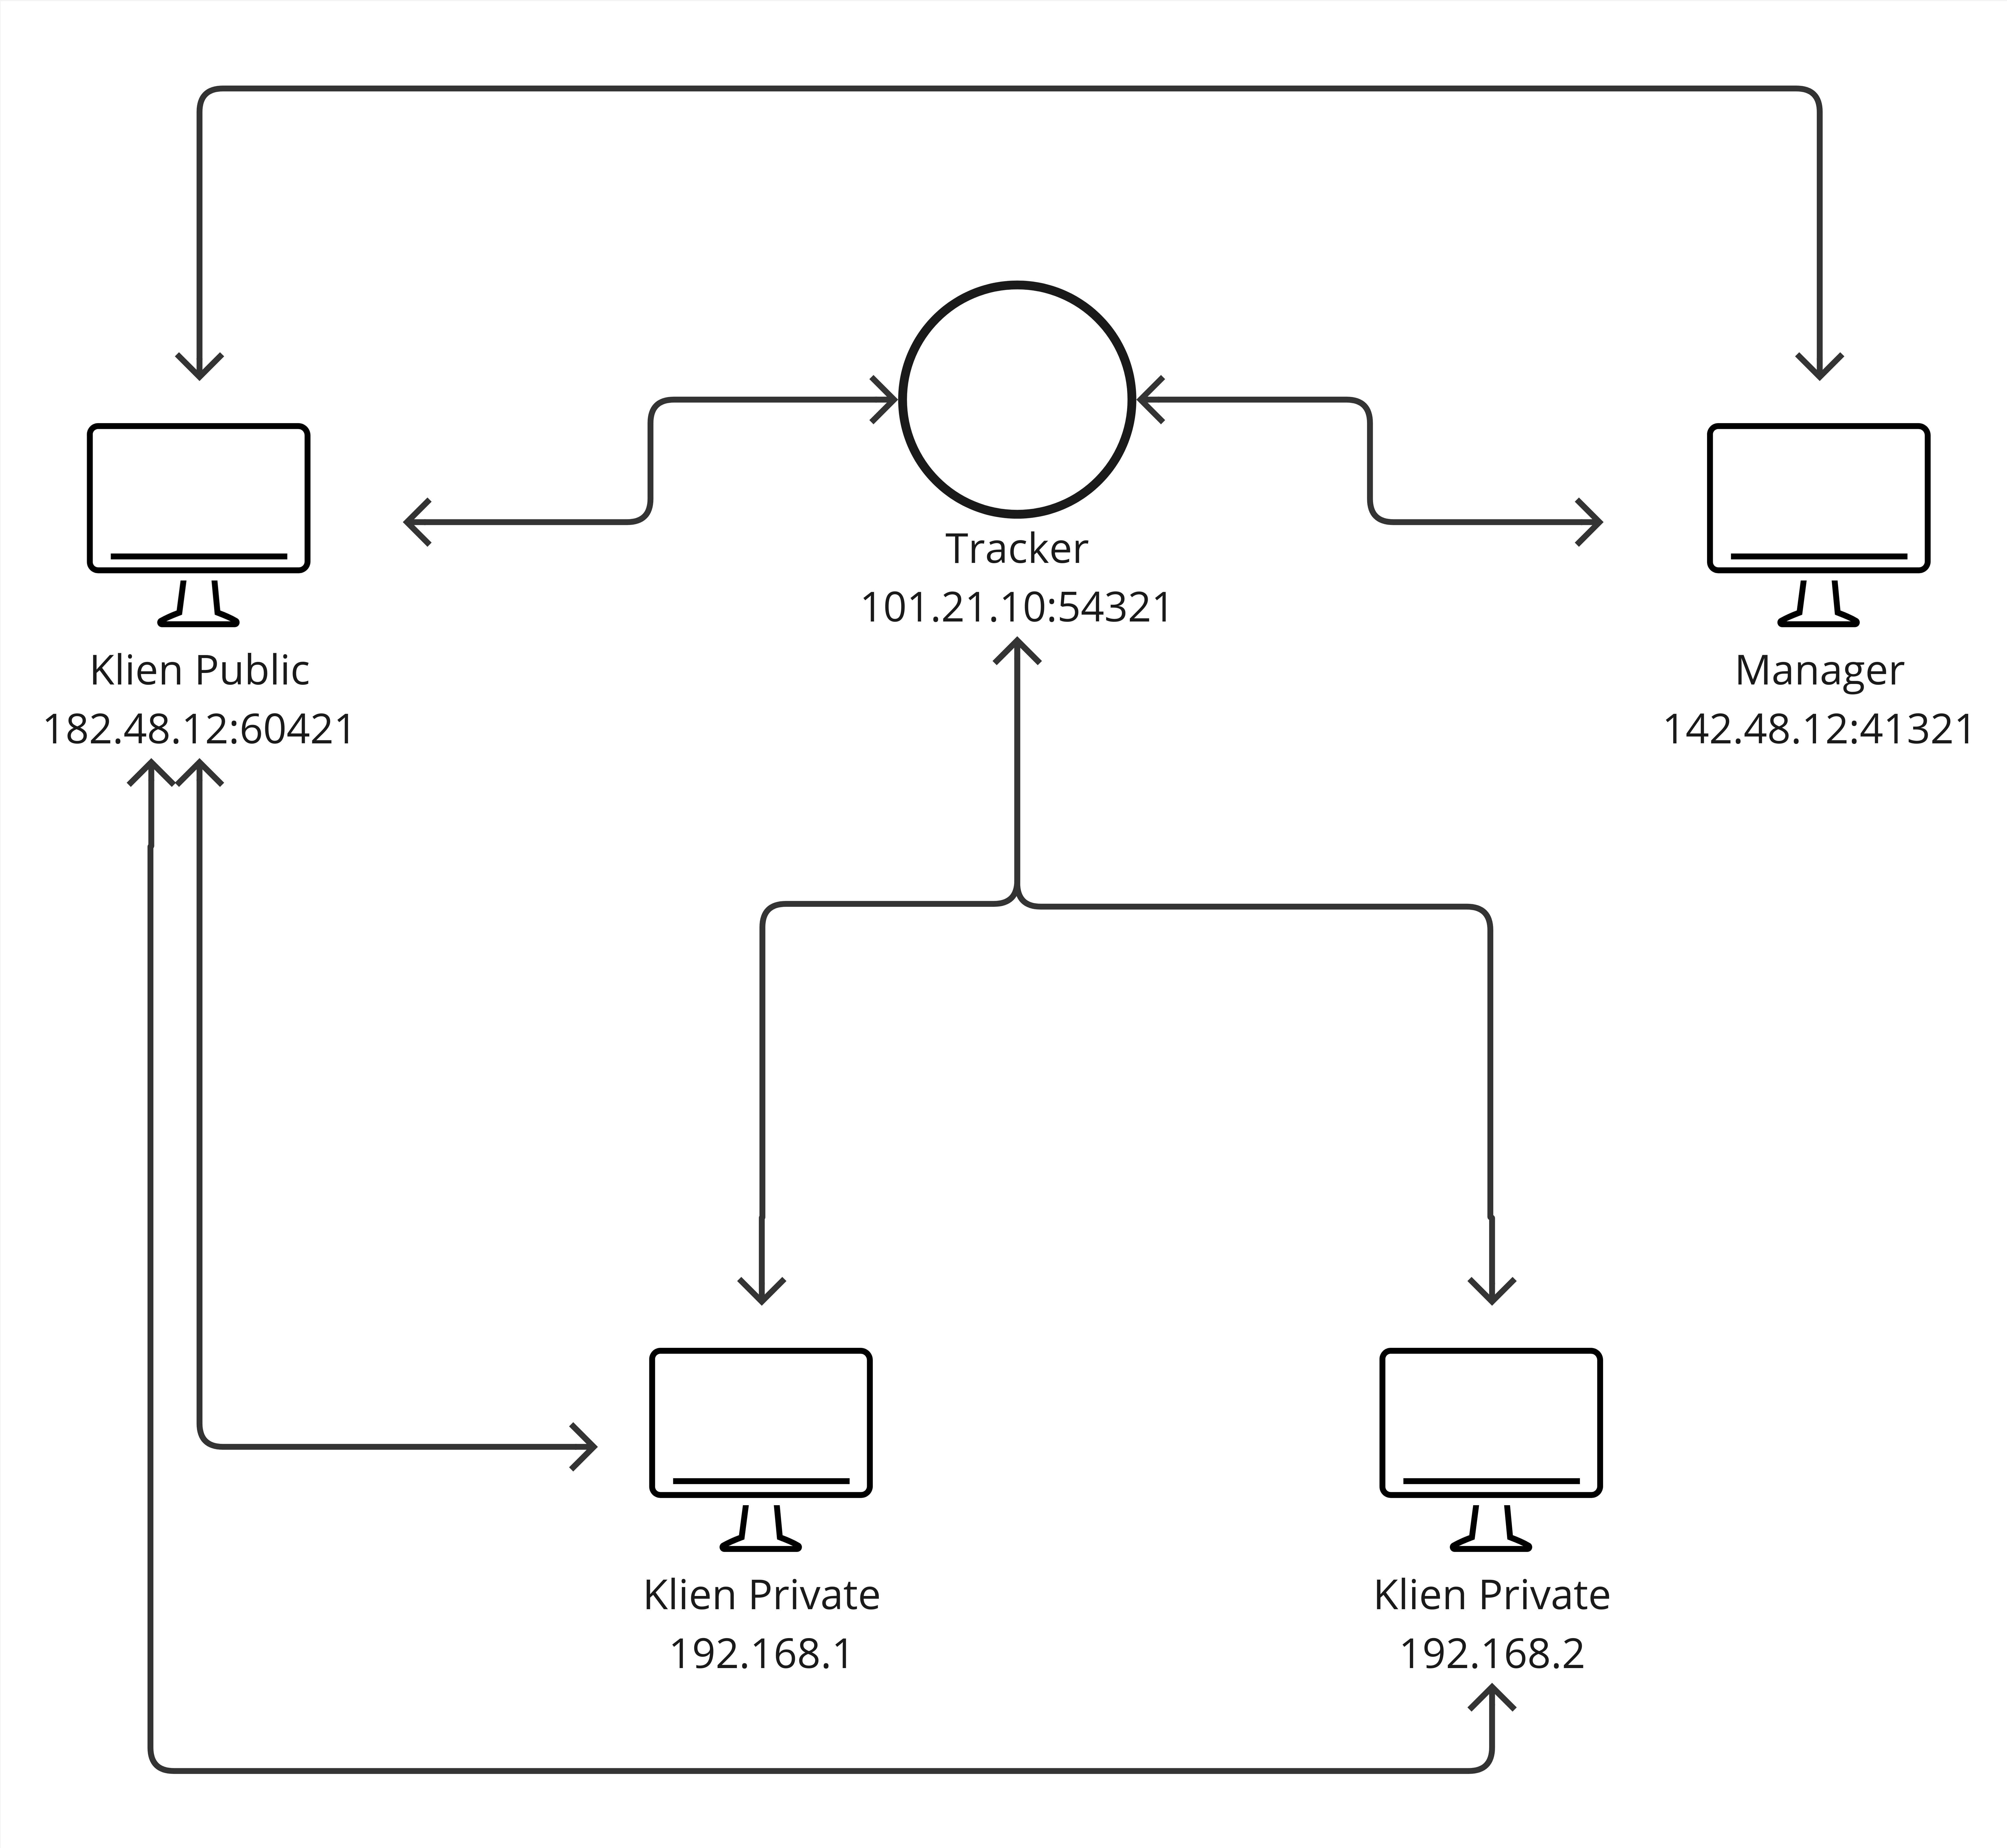
\includegraphics[width=0.85\textwidth]{gambar/bab1/arsitektur_baru}
  \caption{Arsitektur Sistem \emph{Crawler} Terdistribusi Sebelumnya (\cite{ridho2024})} 
\end{figure}

% Paragraph 4
Pada arsitektur tersebut \emph{database} disimpan secara terpusat pada 1 \emph{public 
client} walaupun masing-masing \emph{private client} juga menyimpan data. Akan 
lebih baik jika penyimpanan dilakukan secara terdistribusi daripada 
harus terpusat. Berdasarkan \emph{Paper An Overview of Distributed Databases} (\cite{overviewdistributed})
dinyatakan bahwa salah satu manfaat dari penerapan \emph{database} terdistribusi 
ini adalah \emph{High Performance-Queries and updates are largely local so that 
there is no network bottleneck}. Berdasarkan pernyataan tersebut didapatkan 
bahwa \emph{database} terdistribusi membuat performa \emph{query database} terutama \emph{query} 
yang jumlahnya cukup besar akan menjadi lebih efektif serta akan terhindar 
dari \emph{network bottleneck} karena operasi penyimpanan atau pengubahan dilakukan 
secara lokal. Terdapat manfaat lain yang dinyatakan di \emph{paper} tersebut 
di antaranya:
\begin{enumerate}
\setlength\itemsep{0pt}
  \setlength\topsep{0pt}
	\item{
		\emph{Robust} (Kokoh), jika satu bagian mengalami masalah maka tidak akan 
		menghentikan atau mengganggu bagian lainnya.
	}
	\item{
		\emph{Security}, akses pekerja dapat dibatasi sesuai dengan porsi \emph{database} 
		mereka masing-masing.
	}
	\item{
		Arus jaringan berkurang sehingga membuat \emph{bandwidth cost} berkurang.
	}
	\item{
		\emph{Database} lokal masih dapat bekerja meskipun jaringan perusahaan 
		sedang rusak atau kendala.
	}
	\item{
		Dalam sistem terdistribusi akan lebih mudah untuk membuat sebuah 
		\emph{error} tidak menyebar ke seluruh sistem.
	}
\end{enumerate}


% Paragraph 5
Dalam sistem tersebut, pengguna juga hanya bisa memiliki 1 \emph{public client} 
sementara jika mencoba untuk menambah 1 \emph{public client} lagi, maka \emph{public 
client} tersebut akan berperan layaknya \emph{private client} yang menjalankan 
\emph{crawling}. Cara lain untuk menambah \emph{public client} agar \emph{database} tidak menjadi 
terpusat adalah dengan menjalankan sistem yang sama pada mesin yang berbeda, 
sehingga dalam sistem tersebut dapat berisi 2 \emph{public client}, 2 manajer 
dan 2 \emph{tracker}. 

% Paragraph 6
Namun jika ingin menerapkan cara tersebut terdapat sebuah permasalahan pada 
penyimpanan data antar mesin dan sinkronisasinya. Sinkronisasi yang berjalan 
pada sistem saat ini hanya diterapkan pada \emph{public} dan \emph{private client}. 
Sementara antara sebuah \emph{public client} dengan \emph{public client} yang lain masih 
belum bisa melakukan sinkronisasi. Karena belum bisa melakukan sinkronisasi 
antara \emph{public client} maka akan sangat rentan terjadinya duplikasi data di 
penyimpanan \emph{database}.

Pada \emph{public client}, penggunaan MongoDB sebagai \emph{database} utama akan digunakan. Berdasarkan
\emph{Paper A Comparative Study: MongoDB vs. MySQL} (\cite{Comparative2015}) dikatakan bahwa \emph{"MongoDB provided lower 
execution times than MySQL in all four basic operations, which is essential when an application 
should provide support to thousands of users simultaneously. Thus, the above comparison tests, 
proves that for large amounts of data MongoDB has a good performance and it is preferred than MySQL".}
Dari pernyataan tersebut disimpulkan bahwa MongoDB mempunyai performa yang lebih baik dibanding MySQL
yang mempunyai basis \emph{Relational Database}. Namun terdapat permasalahan baru, karena \emph{Private Client}
pada arsitektur sebelumnya (\cite{ridho2024}) menggunakan sqlite yang membuat dalam sistem terdapat 2 jenis \emph{database}
berbeda antara \emph{public client} dan \emph{private client}

Penggunaan 2 jenis \emph{database} yang berbeda juga akan membutuhkan lapisan sinkronisasi
untuk membuat \emph{database} yang terhindar dari duplikasi data. Berdasarkan \emph{paper Implementing a 
Synchronization Method between a Relational and a Non-Relational Database} (\cite{Gyrdi2023}) didapatkan bahwa 
sinkronisasi antar \emph{database} pasti akan menimbulkan \emph{delay}. Waktu delay yang dialami juga mengalami
peningkatan secara eksponensial. Peningkatan signifikan ini akan terus meningkat dengan seiring dengan 
bertambahnya jumlah data. Berikut adalah gambar \emph{chart} yang didapat dari paper tersebut.

\begin{figure}[H]
  \centering{}
	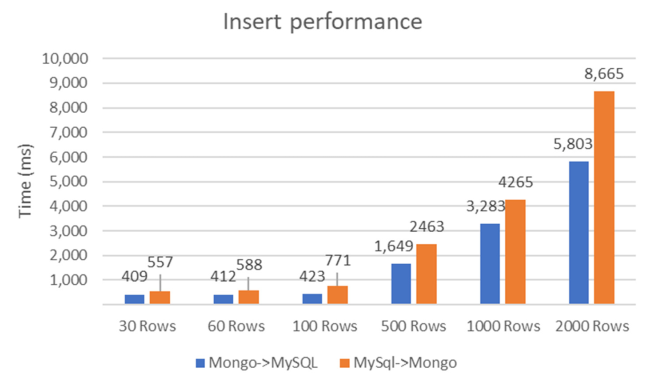
\includegraphics[width=0.85\textwidth]{gambar/bab1/chart-exponent}
  \caption{Grafik peningkatan operasi \emph{insert} pada \emph{database} berbeda, biasa disebut \emph{heterogenous} (\cite{Gyrdi2023})} 
\end{figure}

Waktu \emph{delay} antara sinkronisasi \emph{database} dapat diatasi dengan melakukan efisiensi terhadap 
algoritma sinkronisasi. Salah satu algoritma sinkronisasi yang dapat dicoba diterapkan adalah arsitektur dan algoritma sinkronisasi yang berada pada
\emph{paper Design and Implementation of a Heterogeneous Relational Database Synchronization Mechanism Based on Tree Distribution Architecture} (\cite{Xu2019}). 
Untuk menerapkan algoritma sinkronisasi tersebut juga akan membutuhkan lapisan sinkronisasi tambahan dikarenakan sqlite dan mongoDB merupakan entitas \emph{database}
yang berbeda. Lapisan tambahan ini bisa dihilangkan dengan memasukkan lapisan sinkronisasi tersebut sebagai fitur \emph{native} dari MongoDB dan SQLite.
Namun \emph{source code} MongoDB memiliki lisensi yang memiliki aturan-aturan tertentu ketika pengembang melakukan memodifikasi dan mengubah \emph{source code}.
Aturan-aturan pada lisensi membuat pengembang tidak bisa memiliki kendali penuh terhadap \emph{source code} sistem tersebut. Permasalahan ini yang memicu timbulnya ide untuk membuat \emph{database} baru yang dapat lebih 
adaptif terhadap sistem \emph{crawling} yang berjalan saat ini. Hal ini dikarenakan pengembang dapat memegang kendali penuh mulai dari proses pengambilan, penyimpanan,
pengubahan dan penghapusan data. Algoritma sinkronisasi antar \emph{database} pun juga dapat diterapkan langsung pada \emph{database} tanpa melalui perantara lapisan sinkronisasi.

Jika meninjau \emph{database} selain MongoDB yang memiliki lisensi lebih aman seperti Postgresql terdapat permasalahan baru yaitu kompleksitas dari \emph{source code}. Kompleksitas ini
berbanding lurus dengan banyaknya fitur postgresql, di dalam \emph{source code} tersebut terdapat banyak sekali \emph{file} serta \emph{function} yang dibuat. Oleh karena itu, untuk mencoba
mengadaptasi \emph{source code} dari postgresql dan mengubah sesuai dengan kebutuhan akan sulit dilakukan dengan kemampuan penulis saat ini. Selain itu, \emph{database engine} yang telah dibuat
biasanya telah memiliki alur lapisan pemrogamannya tersendiri. Sementara dengan membuat \emph{database engine} tersendiri, pengembang dapat menyesuaikan alur serta algoritma
yang sesuai dengan sistem \emph{crawling} pada penelitian sebelumnya (\cite{ridho2024})

% Paragraph 9
Lalu manfaat lain dari pembuatan \emph{database} baru ini adalah pengembang dapat menyesuaikan skema distribusi \emph{database} yang paling cocok dengan 
sistem \emph{crawling} yang ada saat ini (\cite{ridho2024}). Salah satu konsep distribusi \emph{database} yang dapat digunakan adalah konsep distribusi yang ada
pada \emph{paper} berjudul \emph{Research on The Improvement of MongoDB Auto-Sharding in Cloud Environment} (\cite{improvementsharding}). \emph{Paper}
ini membahas tentang arsitektur yang berjalan pada MongoDB. Konsep distribusi dilakukan dengan memecah 
kumpulan-kumpulan data menjadi potongan-potongan kecil. Potongan tersebut dapat didistribusikan antar mesin agar setiap mesin 
bertanggung jawab pada subset dari total data set yang ada. Penggunaan \emph{database} pada sistem terdistribusi akan diterapkan pada sistem \emph{crawling} ini berdasarkan 
saran dari penelitian sebelumnya (\cite{ridho2024}). Akan tetapi penerapan \emph{database} pada sistem terdistribusi baru akan dilaksanakan setelah mesin dan fitur utama dari 
\emph{database} baru ini selesai.

\section{Rumusan Masalah}
Berdasarkan dari rincian dan penjelasan latar belakang di atas, maka didapatkan 
rumusan masalah "\textbf{Bagaimana Perancangan dan Implementasi \emph{Prototype Database Engine} Berbasis 
\emph{Structure Oriented Programming} Menggunakan Rust?}".

\section{Batasan Masalah}
Rumusan masalah yang didapat memiliki permasalahan yang cukup banyak dan luas 
sehingga harus diperjelas batasaannya. Batasan Masalah pada penelitian yang 
dilakukan antara lain:
\begin{enumerate}
	\item{
		Pembuatan \emph{database engine} meliputi penerapan penyimpanan data 
		secara persisten dan menjaga integritas data yang dibuat dengan bahasa pemrograman 
		Rust.
	}
	\item{
		\emph{Database engine} yang dibuat belum menggunakan bahasa/\emph{query} secara langsung 
		sehingga jika ingin mengambil data hanya bisa melalui \emph(interface) yang 
		tersedia.
	}
	\item{
		\emph{Database} yang dibuat belum menerapkan \emph{foreign key} atau relasi antar tabel, 
		sehingga penerapan nanti tidak bisa memiliki \emph{constraint} antar tabel. Pengambilan 
		data antar tabel hanya sebatas \emph{joining} tabel.
	}
\end{enumerate}

\section{Tujuan Penelitian}
\begin{enumerate}
	\item{
		Membuat \emph{database engine} yang dapat digunakan secara \emph{universal} (Dapat digunakan pada sistem lain) dan memiliki data konsisten
	}
	\item{
		Membuat \emph{database engine} yang memiliki proses penyimpanan, pengambilan, pengubahan, penghapusan, \emph{joining} antar table dan memiliki \emph{indexing}.
	}
	\item{
		Membuat \emph{database engine} yang memiliki kendali penuh mulai dari tahap penyimpanan, pengambilan, pengubahan dan penghapusan. 
		Arti dari kendali penuh yang dimaksud adalah jika terdapat perubahan atau penambahan fitur ke depannya, maka tidak perlu melalui
		layer tambahan dan dapat ditambahkan ke pemrosesan \emph{database} secara langsung (\emph{seamless}).
	}
\end{enumerate}

\section{Manfaat Penelitian}
\begin{enumerate}
	\item Bagi penulis \\
	Menambah wawasan dan ilmu tentang sistem terdistribusi serta penerapannya, 
	memperoleh gelar sarjana pada bidang ilmu komputer dan mendapatkan pengalaman 
	dalam menulis sebuah jurnal ilmiah.
		
	\item Bagi Program Studi Ilmu Komputer \\
	Penelitian ini dapat menjadi referensi untuk penelitian yang akan dilakukan 
	mahasiswa ilmu komputer mendatang.


	\item Bagi Universitas Negeri Jakarta \\
	Dapat menjadi bahan evaluasi dan penilaian kualitas akademik di Universitas 
	Negeri Jakarta khusus nya pada program studi Ilmu Komputer.
			
\end{enumerate}

% Baris ini digunakan untuk membantu dalam melakukan sitasi
% Karena diapit dengan comment, maka baris ini akan diabaikan
% oleh compiler LaTeX.
\begin{comment}
\bibliography{daftar-pustaka}
\end{comment}

%!TEX root = ../main.tex
%-------------------------------------------------------------------------------
%                            BAB II
%               KAJIAN TEORI
%-------------------------------------------------------------------------------

\chapter{Kajian Pustaka}

\section{\emph{Database}}

Pada Era teknologi saat ini, terdapat banyak sekali informasi-informasi 
yang tersebar. Mulai dari informasi mengenai pendidikan, penelitian, 
ekonomi dan lainnya. Informasi yang didapat bisa dikatakan sebagai data. 
Data dapat berbentuk angka, kumpulan kata, symbol dan lainnya. Data-data 
ini harus disimpan supaya bisa diolah atau disebarkan.  Untuk tercapai 
hal nya tersebut dibutuhkan sebuah teknologi untuk menyimpan data-data 
tersebut. Teknologi tersebut adalah \emph{database}. \emph{Database} adalah sebuah 
kumpulan data yang digunakan untuk mendukung aktivitas dari individu 
ataupun kelompok (\cite{databasedesignwatt}). \emph{Database} dapat berisi 
sebuah tabel, sebagai contoh sebuah \emph{database} perpustakaan dapat berisi 
tabel buku dan tabel pengunjung di mana kedua tabel tersebut dapat 
berkaitan satu sama lain. 

\emph{Database} juga dapat didefinisikan sebagai kumpulan data yang berkaitan 
di mana pengguna dapat mengambil data tersebut secara efisien 
(\cite{introductiondatabase}). Data-data yang telah dikumpulkan tersebut
sangat memungkinkan untuk diolah, diambil, dan diubah. Untuk melakukan 
hal tersebut dibutuhkan sebuah sistem yaitu \emph{database management 
system} yang disingkat sebagai DBMS. DBMS adalah sebuah program yang 
membuat pengguna dapat mengelola \emph{database} dan mengontrolnya 
(\cite{databasedesignwatt}). Tujuan utama dari DBMS adalah menyediakan 
aksesibilitas bagi pengguna agar dapat mengolah dan mengontrol 
data dengan baik. Di sisi lain DBMS juga harus untuk memastikan 
keamanan dari data yang telah disimpan dari pihak luar atau pihak 
tidak dikenal.

Berdasarkan buku \emph{database system}  (\cite{introductiondatabase}), DBMS merupakan manajemen data 
tersentralisasi. Terdapat beberapa kelebihan jika data disimpan secara tersentralisasi, kelebihan 
inilah yang juga menutupi kekurangan metode penyimpanan data sebelumnya yaitu \emph{file-based}. 
Berikut ini adalah beberapa kelebihan yang telah 
disebutkan pada buku tersebut (\cite{introductiondatabase}):

\begin{enumerate}
	\item Kontrol Redudansi Data \\
	\emph{Database} didesain untuk mengurangi redudansi data dikarenakan 
  sebagian besar data yang disimpan didalamnya terintegrasi 
  dengan data yang ada di tempat lain. Kondisi ini meminimalisir 
  terjadinya replikasi data pada tempat lain dan juga memastikan 
  konsistensi pada penyimpanannya. Walaupun dalam kondisi mungkin 
  saja  terjadi duplikasi data untuk mengoptimalkan performa saat 
  menggunakan \emph{database}.

	\item Integritas Data \\
  Pada penggunaan \emph{database}, penerapan integritas data menjadi 
  lebih mudah. Saat proses melakukan desain, pengguna dapat 
  menentukan hubungan dan relasi antar data pada \emph{database} yang 
  akan dibuat. Beberapa penerapan integritas data dapat dibuat 
  langsung di \emph{database} secara otomatis atau dapat melalui 
  aplikasi yang menggunakan data tersebut.

	\item Aksesibilitas \\
	Data yang disimpan di \emph{database} dapat diakses oleh beberapa 
  pengguna ataupun program. Dengan kasus seperti ini, bisa 
  saja terdapat dua aplikasi yang berbeda namun menggunakan 
  sumber data yang sama.

  \item Kemudahan dalam Pengembangan \\
  Dengan menggunakan DBMS, permasalahan seperti keamanan, 
  konkurensi, integritas data dan lainnya sudah ditangani 
  oleh DBMS itu sendiri. Pengembang aplikasi menjadi lebih 
  mudah karena tidak perlu memikirkan hal tersebut.

  
  \item Keamanan \\
  Karena penyimpanan data secara terpusat, membuat penerapan 
  keamanan menjadi lebih mudah. DBMS dapat memastikan bahwa 
  pengolahan data hanya bisa terjadi pada akses yang 
  diizinkan. Pada umumnya DBMS menyediakan sebuah code atau 
  password bagi pengguna yang ingin mengakses data.
\end{enumerate}


\section{Fitur-fitur pada \emph{Database}}
Berdasarkan buku \emph{database design} (\cite{databasedesignwatt}), \emph{database} (dalam pembahasan ini adalah \emph{relational database}) dapat memiliki banyak tabel. 
Setiap tabel tersebut juga dapat memiliki banyak kolom yang menyimpan data sesuai dengan kebutuhan dari pengguna. Setiap kolom yang ada di dalam tabel memiliki bisa memliki tipe data yang
berbeda-beda. Selain kolom, dalam \emph{database} memiliki baris data, dan nilai dari baris data tersebut akan berkaitan dengan kolom yang telah dibuat pada tabel. Tipe data dari baris juga harus
sama dengan tipe data dari kolom. 

Pengguna sering sekali membutuhkan akses kepada data yang telah tersimpan tersebut seperti melakukan pembuatan, pengambilan data untuk
melakukan analisa dan lainnya. Seperti yang dikutip pada subbab sebelumnya bahwa untuk melakukan pengolahan database, pengguna dapat menggunakan DBMS. Salah satu model DBMS yang
sering digunakan adalah \emph{relational} DBMS dan SQL (\emph{Structured Query Languange}) sebagai bahasa standar yang digunakan untuk mengakses DBMS. Berdasarkan buku \emph{database design} 
(\cite{databasedesignwatt}), SQL digunakan dalam DBMS untuk melakukan berbagai hal seperti:

\begin{enumerate}
	\item Membuat \emph{database} dan tabel

	\item Melakukan pengolahan data yang umum digunakan seperti (membuat, menghapus, dan mengubah)

  \item Melakukan pengambilan data untuk mengubah data mentah menjadi data yang dapat terbaca dengan baik
  
\end{enumerate}

Untuk melakukan pembuatan tabel, pembuatan \emph{database} harus terlebih dahulu dilakukan. Tabel akan memiliki sebuah nama, dan dalam tabel tersebut pengguna juga bisa membuat kolom yang banyak.
Kolom tersebut berisi nama dari kolom, tipe data dari kolom dan beberapa konfigurasi tambahan lainnya. Nama yang diberikan pada kolom harus bersifat unik dan tidak boleh sama antara satu
dengan yang lainnya. Untuk tipe data, SQL memiliki beberapa jenis tipe data yang didukung, beberapa di antaranya yaitu:

\begin{enumerate}
  \item Bit - Sebuah data integer bernilai 1 atau 0.

  \item Int - Data integer dari -2.147.483.6488 hingga 2.147.483.647

  \item Smallint - Data integer dari -32.768 hingga 32.767

  \item Tinyint - Data integer dari 0 hingga 255
  
  \item Uniqueidentifier - \emph{Global Unique Identifier} (\emph{GUID})
  
  \item Float - Tipe data yang mengambil data secara presisi

  \item Varchar - non-unicode karakter data yang berjumlah maksimal 8.000 karakter

  \item Text - non-unicode karakter data yang berjumlah maksimal 2.147.483.647 karakter
\end{enumerate}

Pada SQL, pengguna juga dapat menghapus kolom, menamnbahkan kolom, menghapus tabel dan beberapa
konfigurasi lainnya. SQL juga mendukung operator \emph{join} yang berguna untuk menghubungkan kedua tabel atau lebih. Pembahasan mengenai \emph{join} tabel akan dibahas pada subbab 2.6.

Di dalam DBMS umumnya juga memiliki fitur \emph{index} yang berguna untuk melakukan pengambilan data secara efisien. Berdasarkan buku
\emph{Database System} (\cite{databasesystem}), \emph{index} adalah sebuah struktur data yang disimpan dengan tujuan untuk mempercepat
akses terhadap sebuah data yang telah tersimpan. Pembahasan lebih rinci mengenai \emph{index} akan dibahas pada subbab 2.4.

\section{Arsitektur Internal \emph{Database Management System}}

Berdasarkan buku \emph{Database Internal} ({\cite{databaseinternal}}), 
arsitektur yang diterapkan dalam pengembangan \emph{database management system}, 
tidak mempunyai standar penerapan yang pasti. Setiap \emph{database} 
dapat dibuat dengan arsitektur yang berbeda dan arsitektur yang diterapkan pun juga 
sulit dilihat dan ditentukan. Meski arsitektur \emph{database}  ini dijelaskan pada sebuah tulisan seperti 
dokumentasi, dalam penerapan dan penulisan \emph{code} aslinya, arsitektur yang berbeda mungkin 
saja diterapkan untuk optimalisasi performa, penanganan beberapa kasus, atau 
keputusan arsitektur. Berikut ini adalah gambaran besar arsitektur 
DBMS yang sering digunakan.


\begin{figure}[H]
  \centering{}
	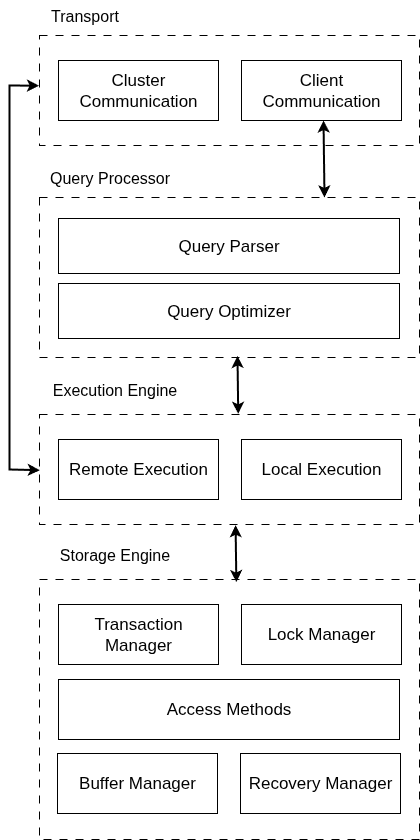
\includegraphics[width=0.5\textwidth]{gambar/bab2/dbms_achitecture}
  \caption{Ilustrasi Arsitektur \emph{Database}  Umum (\cite{databaseinternal})}
\end{figure}

\emph{Database management system} menggunakan \emph{client/server model}, di mana 
sebuah sistem \emph{database} berperan sebagai server, dan aplikasi mengambil 
peran sebagai \emph{client}. Permintaan \emph{client} akan diterima melalui 
\emph{transport subsystem}. Permintaan datang dalam bentuk sebuah \emph{query}, dan 
sering sekali dikatakan sebagai \emph{query language}. \emph{Transport subsystem} 
juga bertugas untuk melakukan komunikasi dengan node yang lain dalam 
cluster \emph{database} . Setelah menerima permintaan, \emph{transport subsystem} 
menyerahkan \emph{query} kepada \emph{query processor yang} akan menguraikan (\emph{parse}), 
menafsirkan (\emph{interprets}) dan melakukan validasi terhadap \emph{query} tersebut. 
Setelah semua proses ini selesai, pemeriksaan akses kontrol akan dilaksanakan.

\emph{Query} yang telah diuraikan akan diberikan kepada \emph{query optimizer}, yang 
akan menghilangkan bagian yang tidak memungkinkan untuk dijalankan dan bagian yang 
redundan dari \emph{query}. Lalu, sistem akan mencoba untuk mencari cara yang 
paling efisien untuk mengeksekusi \emph{query}-nya berdasarkan statistik \emph{internal} 
(kardinalitas \emph{index}, perkiraan ukuran \emph{intersection} dan lainnya) dan 
penempatan data (\emph{node} yang menyimpan data dalam \emph{cluster} dan biaya yang 
berkaitan dengan perpindahannya). \emph{Optimizer} menangani 2 hal yaitu, 
operasi yang dibutuhkan untuk resolusi pada \emph{query} (biasa dipresentasikan 
sebagai \emph{dependency tree}) dan optimisasi seperti pengurutan \emph{index}, estimasi 
kardinalitas dan pemilihan metode akses.

\emph{Query} biasanya dibuat dalam bentuk \emph{execution plan} (atau bisa disebut 
\emph{query plan}). \emph{Execution plan} adalah barisan / kumpulan operasi yang harus 
dibawa untuk memastikan hasil dianggap selesai. Karena \emph{query} yang sama 
dapat membuat hasil yang sama dengan \emph{execution plan} yang berbeda 
berdasarkan tingkatan efisiensinya, \emph{optimizer} akan mengambil \emph{execution 
plan} yang paling terbaik. \emph{Execution plan} akan diproses oleh \emph{execution 
engine} yang akan mengagregat hasil operasi dari lokal dan \emph{remote}. 
\emph{Remote execution} dapat meliputi proses writing (membuat, modifikasi, 
menghapus, dan lainnya) dan reading (mengakses) data dari node lainnya 
dalam cluster. \emph{Remote execution} juga dapat meliputi replikasi. 
Sementara \emph{local queries} (yang datang langsung dari \emph{client} atau \emph{node} 
lainnya) akan diproses oleh \emph{storage engine}. Sebuah \emph{Storage Engine} 
memiliki beberapa komponen yang masing-masing komponen tersebut memiliki 
tugasnya masing-masing, di antaranya adalah sebagai berikut:


\begin{enumerate}
	\item \emph{Transaction Manager} \\
	Komponen pengelolaan ini menjadwalkan \emph{transactions} dan 
  memastikan bahwa \emph{transactions} tidak dapat selesai dengan 
  kondisi \emph{state} didalamnya tidak konsisten.

		
	\item \emph{Lock manager} \\
	Komponen ini akan mengunci obyek \emph{database} untuk menjalankan 
  \emph{transactions}, untuk memastikan operasi konkurensi tidak 
  merusak integritas data.


	\item \emph{Access Methods} \\
	Komponen ini membantu pengelolaan akses dan mengorganisir 
  data dalam \emph{disk}. \emph{Access methods} meliputi \emph{heap files} dan 
  struktur penyimpanan seperti \emph{B-Trees} atau \emph{LSM Trees}.


  \item \emph{Buffer Manager} \\
  Komponen pengelolaan ini akan melakukan \emph{caching} data 
  halaman-halaman dalam \emph{memory}. 
  
  \item \emph{Recovery Manager} \\
  Komponen ini mengelola \emph{log} operasi dan merestorasikan 
  sistem jika sistem mengalami kegagalan.
  
\end{enumerate}
  
Secara bersama, \emph{transaction} dan \emph{lock managers} bertanggung 
jawab untuk pengendalian konkurensi. Keduanya menjamin 
integritas data logis dan fisik sambil memastikan bahwa 
operasi konkurensi dilaksanakan se efisien mungkin. Teori-teori yang dijabarkan diatas
ditulis berdasarkan informasi yang didapatkan dari buku (\cite{databaseinternal}).


\section{\emph{Database Index}}
Berdasarkan buku \emph{Introduction to Database System} (\cite{introductiondatabase}), setelah data berhasil disimpan
di \emph{disk} menggunakan metode-metode pengolahan \emph{file}, terdapat sebuah permasalahan utama yaitu bagaimana cara untuk
melakukan pengambilan data dengan cepat pada permintaan atau \emph{query} yang berbeda. Permasalahan ini dapat diselesaikan
dengan menggunakan sebuah struktur tambahan yang bernama \emph{index}. Sebuah \emph{file} dapat dibuat untuk menerapkan penamabahan stuktur 
\emph{index} ini. Penerapan \emph{index} tidak akan memengaruhi peletakan data yang telah disimpan sebelumnya, namun dapat memengaruhi kecepatan
dalam proses pengambilan datanya. Umumnya dalam suatu \emph{database}  dapat lebih dari 1.

Berdasarkan \emph{Pratical SQL, 2nd Edition} (\cite{praticalsql}), \emph{index} pada \emph{database}  berfungsi layaknya \emph{index} yang sering ditemukan pada buku. 
\emph{Query} dapat dipercepat dengan menambahkan sebuah \emph{index}, \emph{index} disini adalah sebuah struktur data terpisah yang dikelola
oleh sistem \emph{database}. Penerapan \emph{index} dalam \emph{database}  biasanya di terapkan pada kolom yang tersedia pada \emph{database}.
\emph{Database} akan menggunakan \emph{index} sebagai jalur cepat dalam melakukan pengambilan data daripada melakukan pengambilan data
dengan cara normal (melakukan pemindaian baris per baris).  

\section{Data Struktur \emph{Map}}

Berdasarkan buku \emph{Data Structures and Algorithms in Java, 6th Edition} (\cite{datastucturealgo}), Map adalah sebuah abstraksi data yang didesain untuk 
melakukan pengambilan dan penyimpanan data secara efektif. Map melakukan penyimpanan dan pengambilan data dengan mendefinisikan sebuah
\emph{key} yang bersifat unik untuk setiap nilai yang disimpan. \emph{Key} yang bersifat unik ini digunakan untuk melakukan pengambilan data
sehingga jika ingin mengambil sebuah data yang tersimpan maka harus mengetahui \emph{key} yang menjadi pasangan dari nilai tersebut.

Berdasarkan informasi dari buku \emph{A Common-Sense Guide to Data Structures and Algorithms, Second Edition, 2nd Edition} (\cite{commondatastucturealgo}), hampir semua bahasa
pemrograman memiliki fitur map ini. Hanya saja istilah yang digunakan pada masing-masing bahasa pemrograman berbeda-beda seperti \emph{Hash Table},
\emph{Hash Maps}, \emph{associative array} dan \emph{dictionary}. Walaupun istilah yang digunakan berbeda, namun yang tetap menjadi kelebihan adalah satu
yaitu kecepatan untuk pengambilan data. Untuk mencari sebuah value dalam struktur data map mempunyai tingkat efisiensi sekitar O(1) berdasarkan rata-rata.
Namun yang harus dijadikan catatan adalah untuk mencari value dalam map, pengguna harus mengetahui dulu key dari value tersebut. Jika tidak, maka pengguna harus
melakukan pengecekkan pada setiap \emph{key} dan \emph{value} dari \emph{map} tersebut. Hal ini menyebabkan tingkat efisiensi meningkat yang awalnya O(1) menjadi
O(N)

\section{Relasi antar Tabel (\emph{JOIN})}
Pada jenis-jenis \emph{database} , terdapat salah satu tipe \emph{database} yang sering digunakan yaitu \emph{Relational Database}. Berdasarkan buku 
\emph{Pratical SQL, 2nd edition} (\cite{praticalsql}), \emph{Relational Database} menyimpan data pada berbagai macam tabel yang saling berkaitan. Tabel yang saling berhubungan akan
menyimpan sebuah data tambahan yang bertujuan untuk menghubungkan tabel tersebut ke tabel lain. Untuk menggabungkan data antar tabel tersebut membutuhkan sebuah 
proses yang bernama \emph{join}. Pada \emph{relational database} seperti MySQL, terdapat beberapa metode dalam melakukan \emph{join} (\cite{praticalsql}), yaitu:
\begin{enumerate}
	\item \emph{JOIN} / \emph{INNER JOIN}\\
  Dengan menggunakan metode \emph{join} ini, data yang ditampilkan hanyalah data yang memiliki hubungan satu sama lain. Sehingga data yang tidak punya hubungan ke tabel lain, maka
  tidak akan ditampilkan.
  
	\item \emph{LEFT JOIN} \\
  Menampilkan seluruh baris data dari tabel sebelah kiri, dan ikut menampilkan data dari tabel sebelah kanan jika terdapat data tambahan pada tabel sebelah kiri yang memiliki
  hubungan ke tabel sebelah kanan.

	\item \emph{RIGHT JOIN} \\
  Prosesnya mirip dengan \emph{LEFT JOIN} akan tetapi berkebalikan. Menampilkan seluruh baris data dari tabel sebelah kanan, 
  dan ikut menampilkan data dari tabel sebelah kiri jika terdapat data tambahan pada tabel sebelah kanan yang memiliki
  hubungan ke tabel sebelah kiri.

	\item \emph{FULL OUTER JOIN} \\
  Menampilkan gabungan semua data dari tabel kiri dan tabel kanan. Akan tetapi jika dalam suatu baris terdapat data tambahan pada masing-masing tabel yang menghubungkan
  kedua tabel, maka baris dari kedua tabel tersebut akan bergabung menjadi satu. Untuk proses \emph{Full Outer Join}, jika dari masing-masing tabel tidak ada data tambahan yang
  menghubungkan antar tabel satu sama lain, maka proses \emph{join} ini tidak akan menampilkan apa-apa.

	\item \emph{CROSS JOIN} \\
  Menampilkan segala jenis kemungkinan penggabungan antar tabel tanpa memperhatikan data tambahan pada masing-masing tabel.

\end{enumerate}



\section{\emph{Database} Terdistribusi}

Berdasarkan buku \emph{database design}(\cite{databasedesignwatt}), dilihat dari jumlah penyebaran dan penggunaan sebuah \emph{database}, 
terdapat 2 cara penggunaan \emph{database} yaitu \emph{database} tersentralisasi 
dan \emph{database} terdistribusi. \emph{Database} tersentralisasi berjalan 
pada satu buah mesin. \emph{Database} dan DBMS berjalan pada sistem 
yang sama. Pengguna dapat berinteraksi dengan \emph{database} tersebut 
melalui koneksi yang telah terhubung pada mesin. Berikut 
adalah ilustrasi penerapan \emph{database} tersentralisasi:


\begin{figure}[H]
  \centering{}
	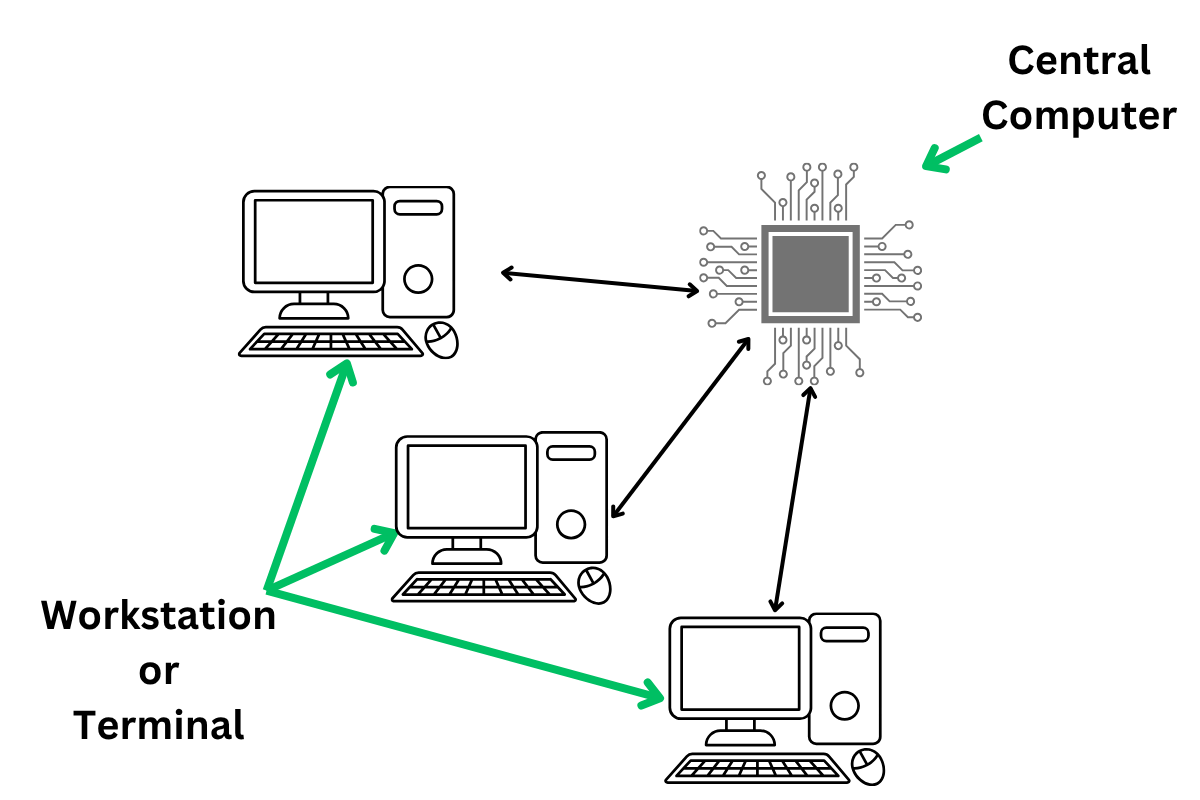
\includegraphics[width=0.65\textwidth]{gambar/bab2/centralized_db}
  \caption{Ilustrasi \emph{Database} Tersentralisasi (\cite{databasedesignwatt})}
\end{figure}

Sementara dalam \emph{database} terdistribusi, \emph{database} dan DBMS 
tersebar ke beberapa mesin yang berbeda. Antar mesin berkomunikasi 
satu sama lainnya melalui sebuah jaringan yang memiliki kecepatan 
tinggi. Berikut adalah ilustrasi dari penerapan \emph{database} terdistribusi:

\begin{figure}[H]
  \centering{}
	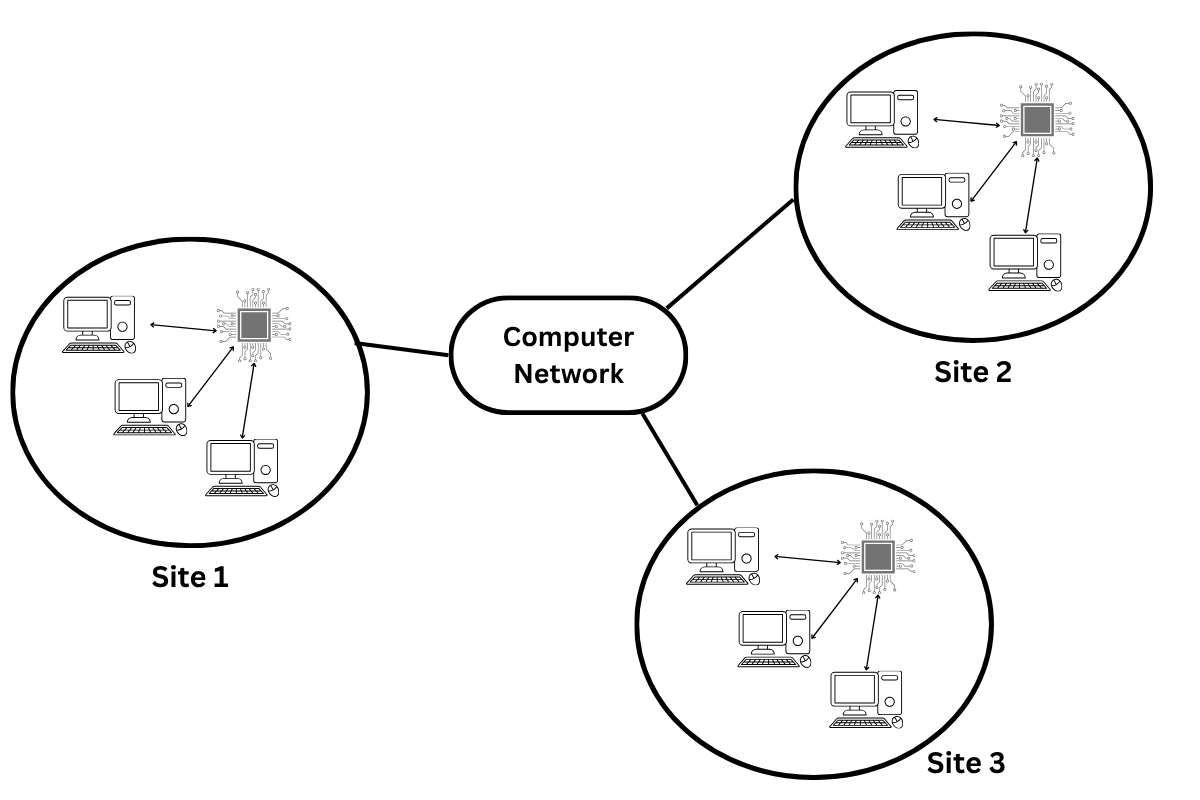
\includegraphics[width=0.65\textwidth]{gambar/bab2/distributed_db}
  \caption{Ilustrasi \emph{Database} Terdistribusi (\cite{databasedesignwatt})}
\end{figure}

\emph{Database} terdistribusi dapat diklasifikasikan menjadi 2 yaitu \emph{homogeneous} 
dan \emph{heterogenous}. \emph{Homogeneous} menggunakan DBMS yang sama antar mesin 
yang terhubung. Dengan begitu perpindahan dan pengolahan data antar mesin 
menjadi lebih mudah. Misalnya sebuah mesin A dan mesin B yang masing-masing 
didalamnya terdapat satu DBMS yang sama. Cara pengambilan data pada kedua 
mesin tersebut akan sama, sehingga ketika melakukan komunikasi, setiap 
mesin tidak perlu melakukan interpretasi kembali. Berikutnya terdapat 
\emph{heterogenous} yang pada penerapan \emph{database} terdistribusi, memungkinkan 
untuk memiliki DBMS yang berbeda antar mesin. Dengan penerapan ini, pengguna 
harus memastikan bahwa kedua DBMS yang berbeda tersebut harus bisa saling 
berkomunikasi. Salah satu penerapannya, beberapa \emph{database} menggunakan 
format \emph{machine-readable cataloguing} (MARC) yang sama untuk mendukung 
pertukaran data. 


\section{\emph{D-Bus}}
Berdasarkan dokumentasi dari freedesktop.org (\cite{dbus}), D-bus adalah 
sebuah \emph{message bus system}, sebuah cara sederhana untuk aplikasi 
berkomunikasi dengan aplikasi lainnya. D-Bus memiliki beberapa lapisan:

\begin{enumerate}
	\item \emph{libdbus} \\
  Merupakan sebuah \emph{library} yang berguna untuk menghubungkan kedua aplikasi satu sama lain dan bertukar \emph{messages}
  
	\item \emph{Message Bus Daemon Executable} \\
  Dibuat dengan libdbus, dan beberapa aplikasi dapat terhubung ke dalamnya. Daemon dapat menyalurkan \emph{messages} dari sebuah aplikasi ke beberapa aplikasi lainnya.

	\item \emph{Wrapper Libraries} atau \emph{Binding Based} \\
	\emph{Wrapper} yang digunakan berdasarkan \emph{framework} atau bahasa pemrograman yang digunakan. Contoh dari \emph{wrapper libraries} ini adalah
  \emph{libdbus-glib} dan \emph{libdbus-qt}. Masih terdapat hal lain seperti \emph{binding} dengan bahasa pemrograman. \emph{Wrapper libraries} ini digunakan untuk 
  mempermudah penggunaan D-bus. \emph{Library libdbus} sendiri memang ditujukan untuk melakukan \emph{binding} dengan \emph{higher level bindings}. Kebanyakan penggunaan API D-Bus
  dipergunakan untuk penerapan \emph{binding}.   
\end{enumerate}

\emph{libdbus} hanya mendukung koneksi \emph{one to one}. Paket pengiriman yang dikirim bukanlah \emph{bytes}, namun dikenal dengan istilah \emph{messages}.
\emph{Messages} mempunyai \emph{header} yang berguna untuk mengidentifikasi jenis dari \emph{message} nya, dan \emph{body messages} berisi sebuah data atau dikenal dengan
\emph{payload}. \emph{Library libdbus} juga akan menangani autentikasi. 

Untuk bagian \emph{message bus daemon}, berperan layaknya sebuah pusat pengiriman \emph{messages}. \emph{Bus Daemon} akan menerima \emph{messages} dari sebuah aplikasi
dan meneruskan \emph{messages} tersebut ke aplikasi yang dituju. \emph{Message bus daemon} dapat juga disebut sebagai \emph{router}. Umumnya pada setiap komputer memiliki
beberapa \emph{message bus daemon}. Berikut adalah diagram proses bekerja D-Bus.

\begin{figure}[H]
  \centering{}
	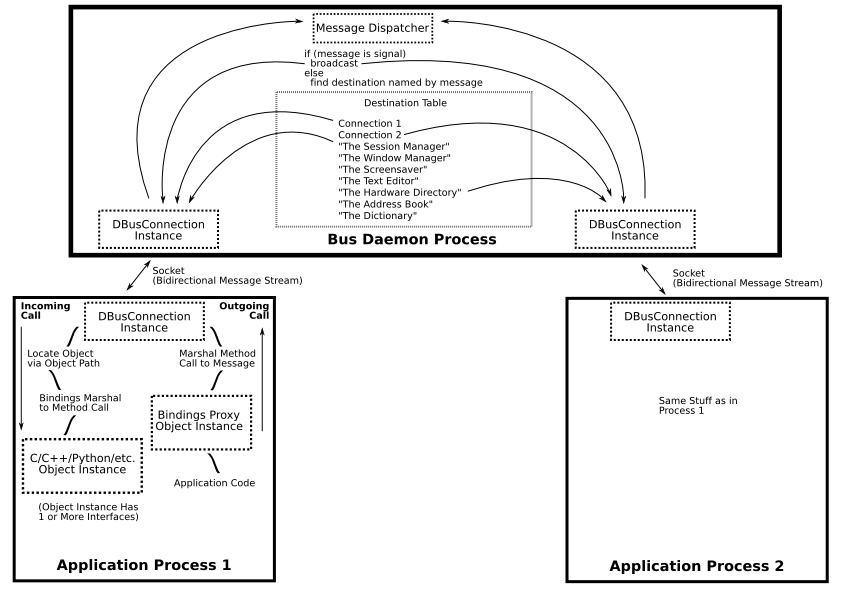
\includegraphics[width=0.95\textwidth]{gambar/bab2/dbus-architecure}
  \caption{Diagram alur D-Bus (\cite{dbus})} 
\end{figure}
%!TEX root = ../main.tex
%-------------------------------------------------------------------------------
%                     BAB III
%               			PEMBAHASAN
%-------------------------------------------------------------------------------


\chapter{METODOLOGI PENELITIAN}

\section{Tahapan Penelitian}

\begin{figure}[H]
  \centering{}
	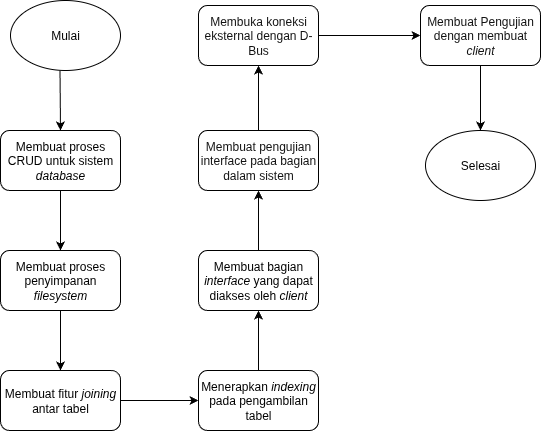
\includegraphics[width=0.9\textwidth]{gambar/bab4/Tahapan-Penelitian-Baru}
  \caption{Alur tahapan penelitian pembuatan \emph{database engine}}
\end{figure}

Penelitian dimulai dengan mencoba menerapkan fungsional dasar (CRUD) pada \emph{database} yaitu proses pengambilan,
penambahan, pengubahan dan penghapusan data. Pengembangan fungsi-fungsi dasar akan melibatkan berbagai macam struktur
data. Langkah pertama dari belum bisa memiliki data yang persisten karena data yang diolah pada langkah ini belum 
terhubung ke \emph{filesystem}.

Langkah berikutnya yaitu penerapan penyimpanan secara persisten di \emph{filesystem}. Meneruskan proses-proses data yang telah
masuk di langkah pertama dan membuat data tersimpan pada \emph{filesystem}. Setelah penyimpanan berhasil dibuat, dilanjutkan dengan proses pembuatan
fitur \emph{joining} antar tabel. Proses \emph{joining} ini akan melakukan penggabungan data dari 2 tabel yang terpisah. Setelah berhasil melakukan \emph{join} tabel, pengembangan fitur \emph{indexing}
akan dilakukan. Fitur \emph{indexing} akan berjalan ketika hendak melakukan pengambilan data pada saat melakukan \emph{join} tabel. Dengan memanfaatkan fitur \emph{indexing},
penerapan fitur \emph{joining} tabel akan dilakukan agar proses penggabungan tabel menjadi lebih cepat.

Setelah fungsi-fungsi berhasil dibuat, maka diperlukan sebuah \emph{interface} untuk memisahkan fungsi mana saja yang dapat diakses oleh pengguna dan fungsi mana
yang hanya bisa diakses oleh sistem. Fungsi pada \emph{Interface} ini yang nanti akan dibuka dan dapat diakses oleh pengguna. Lalu untuk memastikan
fungsi-fungsi yang telah dibuat berjalan dengan baik, dibuatlah \emph{interface} untuk melakukan pengujian secara internal. Interface pengujian internal dibuat berdasarkan fungsi
pada interface yang telah dibuat sebelumnya (\emph{Interface} untuk fungsi pengguna). Maksud dari internal disini adalah proses pengujian dilakukan dengan menggunakan bahasa 
pemrograman yang sama yaitu rust, dan fungsi di panggil secara langsung tanpa melalui koneksi external seperti D-bus.  

Setelah pembuatan \emph{interface} pengujian internal, pembuatan interface koneksi D-Bus dibuat, disusul dengan pembuatan pengujian eksternal menggunakan bahasa pemrograman
lain untuk memastikan koneksi D-Bus berjalan dengan baik. Berikut adalah linimasa dari tahapan penelitian. Linimasa ini hanyalah perkiraan awal dan estimasi dari waktu 
pengembangan \emph{database engine}.


\begin{table}[H]
  \centering{}
  \begin{tabular}{|m{0.8cm}|m{7cm}|m{5cm}|}
      \hline
      \textbf{No.} & \textbf{Tahapan} &  \textbf{Estimasi Waktu} \\
      \hline
      1. & Membuat proses \emph{CRUD} untuk \emph{interface database} & 3 pekan \\
      \hline
      2. & Membuat Proses Penyimpanan \emph{Filesystem} & 1 bulan \\
      \hline
      3. & Membuat fitur \emph{joining} tabel & 2 pekan \\
      \hline
      4. & Menerapkan \emph{indexing} & 2 pekan \\
      \hline
      5. & Membuat \emph{interface} yang dapat diakses pengguna & 1 Pekan \\
      \hline
      6. & Membuat pengujian untuk \emph{interface} pada bagian dalam sistem & 1 Pekan \\
      \hline
      7. & Membuka koneksi external dengan D-Bus & 1 Pekan \\
      \hline
      8. & Membuat pengujian eksternal dengan membuat \emph{client} & 1 Pekan \\
      \hline
  \end{tabular}
  \caption{Tabel linimasa perkiraan awal dan estimasi pengerjaan}
\end{table}

\section{Penerapan Kebutuhan Fitur}
Berdasarkan subbab 2.2, \emph{database} memiliki beberapa fitur umum yang dapat berfungsi untuk mengolah data. 
Untuk proses pengembangan \emph{database engine}, fitur-fitur umum yang ada pada \emph{database} 
akan dikembangkan. Beberapa fitur tersebut di antaranya adalah:
\begin{enumerate}
	\item Kemampuan untuk Membaca data (\emph{Read}) \\
	Fitur ini berguna untuk melakukan pengambilan data yang berasal dari sebuah \emph{file} yang telah disimpan pada \emph{filesystem}.

	\item Kemampuan untuk melakukan proses penyimpanan dan mengolah data secara persisten (\emph{Create, Update dan Delete}) \\
	Proses penyimpanan dan hasil pengolahan data akan disimpan secara persisten pada \emph{filesystem} dengan menggunakan format
  tersendiri. 


	\item Penggunaan \emph{Index} \\
	Penerapan \emph{indexing} sederhana akan diterapkan terhadap data yang ada dalam \emph{database}

	\item Penggabungan 2 tabel (\emph{Join}) \\
	Kapabilitas untuk melakukan \emph{joining} 2 tabel terhadap data yang telah disimpan

	\item Koneksi servis \emph{Client} via \emph{D-Bus} \\	
  Fitur untuk menerima proses permintaan dari \emph{client} untuk menjalankan fungsi-fungsi yang ada dalam \emph{database}.
			
\end{enumerate}

\section{Arsitektur Struktur Data}

Sistem \emph{database} terdistribusi dilakukan dengan melakukan pemecahan penyimpanan 
\emph{database} pada mesin yang berbeda. Setiap mesin \emph{database} yang terpisah dapat 
berkomunikasi satu sama lain namun tidak secara langsung. Dibutuhkan 2 mesin 
tambahan yang berguna untuk menghubungkan \emph{database} terpisah tersebut. Berikut 
adalah ilustrasi dari arsitektur yang akan diterapkan:
\begin{figure}[H]
  \centering{}
  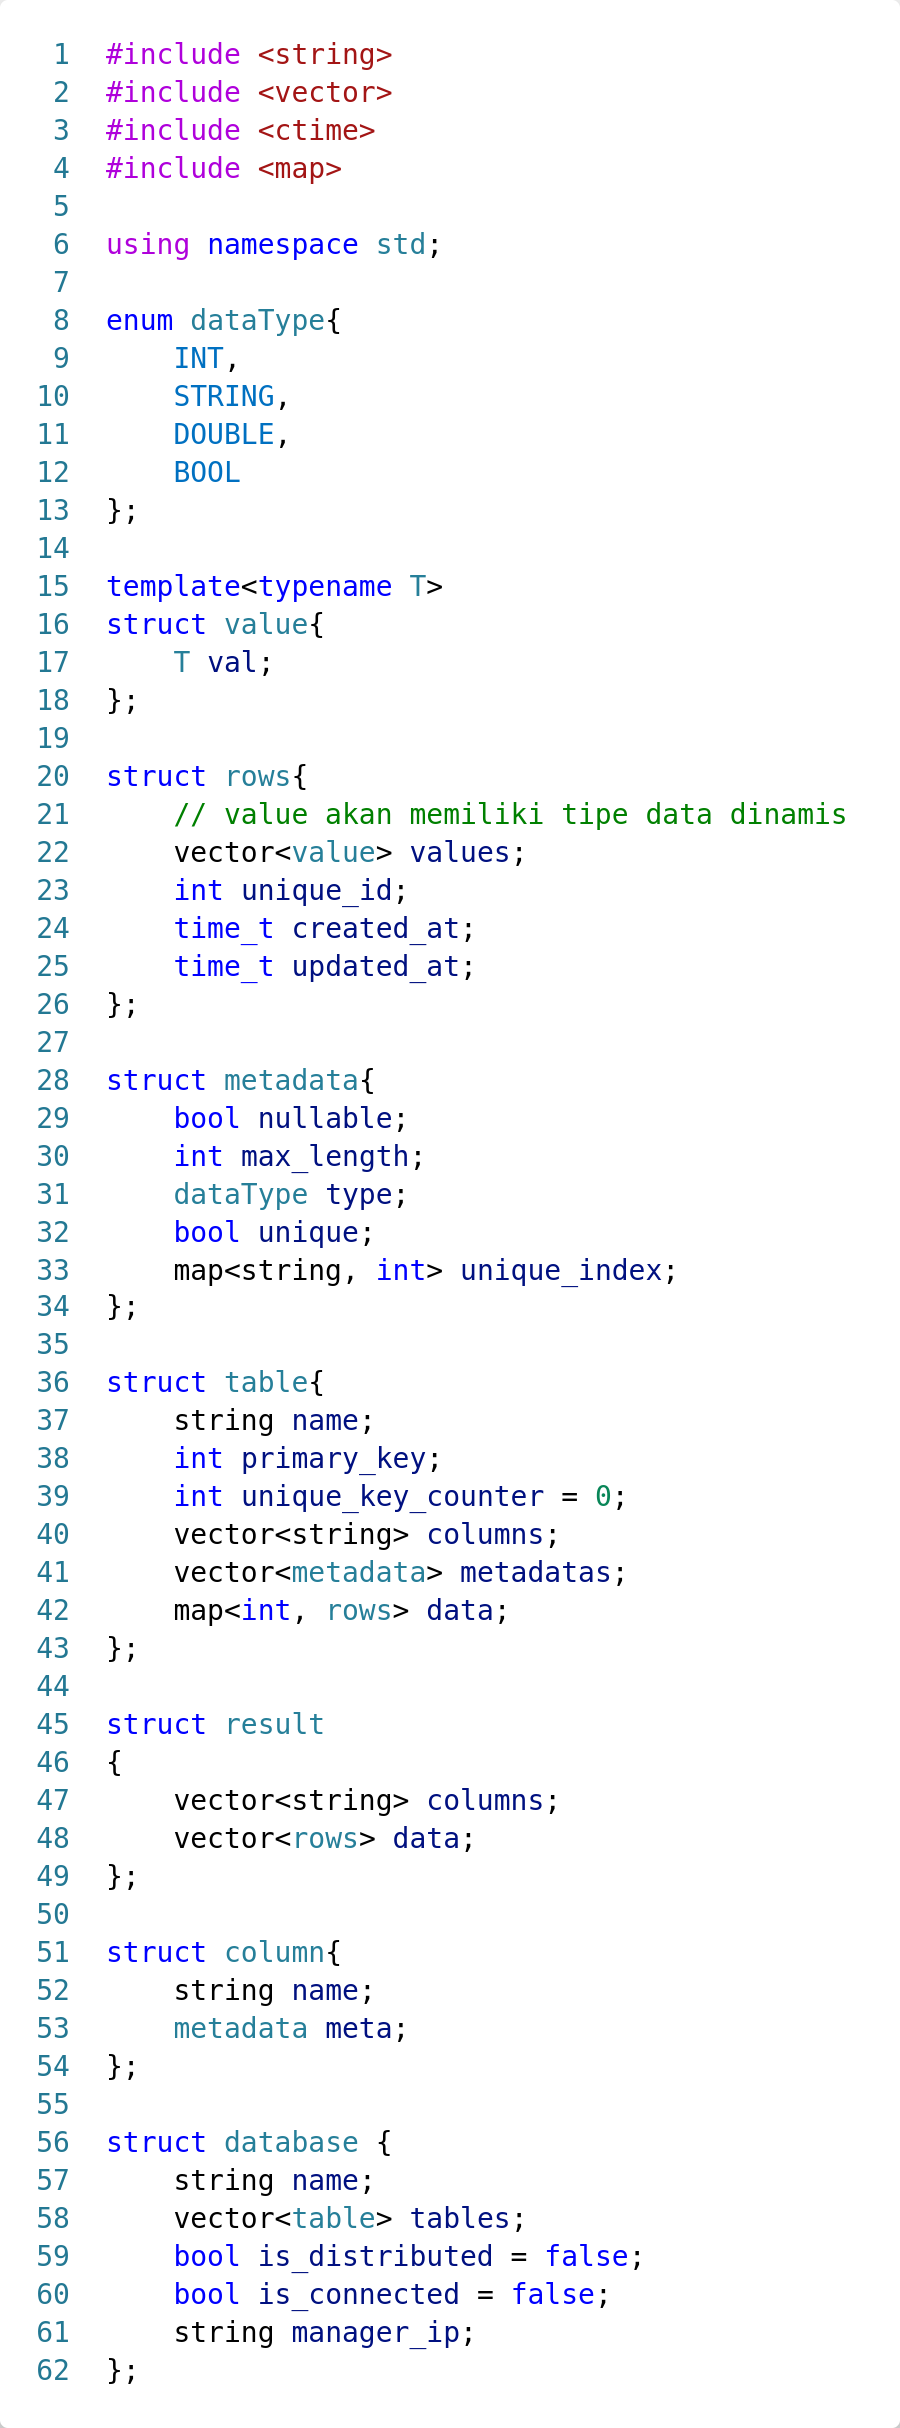
\includegraphics[width=0.5\textwidth]{gambar/bab3/structure_struct_database}
  \caption{Contoh penerapan \emph{struct} \emph{database} pada bahasa C++}
\end{figure}

Terdapat beberapa atribut dalam \emph{class} tabel di antaranya adalah name yang akan 
menampung nama dari tabel, primary\_key yang akan menampung kolom mana yang akan 
menjadi primary key, column yang merupakan array \emph{string} berisi urutan nama kolom 
pada tabel, lalu metadata merupakan array dari \emph{class} metadata yang berisi metadata 
berkaitan dengan kolom yang ada sesuai dengan urutan dan terakhir terdapat atribut 
data. Attribut data ini akan berisi \emph{hashmap} dengan key unique id dengan value 
\emph{class} rows. \emph{Value} unique id berasal dari atribut unique\_key\_counter yang memiliki 
default \emph{value} 0 dan akan terus bertambah ketika terdapat \emph{row} baru yang masuk ke dalam 
hashmap.

Pada penerapan \emph{class} rows, terdapat atribut unique\_id, created\_at dan updated\_at. 
Untuk atribut unique\_id akan berisi sebuah integer yang berasal dari key penyimpanan 
rows di \emph{class} tabel. Atribut created\_at dan updated\_at akan memiliki \emph{value} epoch 
timestamp yang berasal dari waktu data dibuat dan waktu data di diubah. Atribut 
created\_at juga memiliki peran pada saat melakukan penerapan sinkronisasi. Lalu pada 
bagian row memiliki array dari \emph{class values}. \emph{Class} ini memiliki \emph{interface Get Value} 
yang berguna untuk mengembalikan \emph{value} generik yang ada dalam \emph{class values}. Penerapan 
seperti ini dilakukan agar \emph{value} yang disimpan dapat dinamis. 

\emph{Class} column yang dibuat pada gambar, berguna ketika menampilkan semua column beserta 
metadata nya. Terdapat \emph{class} metadata yang akan menyimpan informasi terkait column 
yang ada seperti tipe kolom, \emph{nullable} dan lainnya. Di dalam \emph{class} metadata terdapat 
sebuah hashamp yang akan digunakan sebagai \emph{index}. \emph{Index} ini berfungsi untuk mempercepat 
pencarian terhadap sebuah \emph{value} sehingga akan digunakan ketika column memiliki tipe 
unik dan ketika hendak melakukan sinkronisasi data ketika menerapkan sistem 
terdistribusi. \emph{Hashmap} akan memiliki \emph{key value pair} dengan \emph{key} yang berisi \emph{value} dari 
kolom yang di \emph{index} sementara untuk \emph{value} dari hashmapnya adalah unique id yang 
berasal dari \emph{key} penyimpanan rows pada \emph{class} table. Enum dataType yang ada pada 
metadata berguna untuk membatasi tipe data yang akan dipakai pada column \emph{database}.

Terakhir terdapat \emph{database} \emph{class} atau \emph{struct} yang merupakan \emph{parent} dari semua \emph{class}. 
\emph{Database class} mempunyai atribut table yang merupakan array dari \emph{table} \emph{Class}. 
\emph{Database class} juga mempunyai atribut name yang dibutuhkan ketika saat 
mendeklarasikan \emph{class} tersebut. Dalam \emph{class} yang dibuat akan mengimplementasikan 
\emph{interface} nya masing-masing. \emph{Interface} ini akan berisi metode atau \emph{function} yang 
berguna untuk menjalankan operasi dalam \emph{database}.

Berikut ini adalah isi metode atau \emph{function} yang ada dalam \emph{interface \emph{class} database}:
\begin{enumerate}
	\item \emph{Get Table} \\
	Berguna untuk mengambil \emph{instance} \emph{class table} yang berada dalam \emph{class database}. 
  \emph{Method} ini menerima 1 \emph{parameter} berupa \emph{string} yang isinya adalah nama table dari 
  list \emph{instance} yang ada dalam \emph{database}. Hasil dari \emph{return} \emph{method} ini adalah \emph{instance} 
  table yang mempunyai nama yang sama dengan \emph{value} yang ada di \emph{parameter}.


	\item \emph{Create Table} \\
  \emph{Method} ini berguna untuk menambahkan \emph{class table} baru ke dalam \emph{database}. Menerima 1 
  \emph{parameter} berupa \emph{class table} yang nantinya \emph{instance} tersebut akan dimasukkan ke 
  dalam list \emph{class table} pada \emph{database}. Hasil dari \emph{return method} ini adalah \emph{class 
  table} yang sudah berhasil dibuat. 


	\item \emph{Delete Table} \\
  \emph{Method} ini berguna untuk menghapus tabel yang ada pada \emph{class database}. Menerima 1 
  \emph{parameter} berupa \emph{string} yang isinya adalah nama \emph{table} yang ingin dihapus dalam 
  \emph{database}.

  
	\item \emph{Get Database Name} \\
  \emph{Method} ini berfungsi untuk mengambil nama dari \emph{database}, tidak akan menerima 
  \emph{parameter} apapun dan akan mengembalikan return sebuah \emph{string} nama dari \emph{database}.


	\item \emph{Update Database Name} \\
  \emph{Method} ini berfungsi untuk Mengganti nama dari \emph{database}, akan menerima 1 \emph{parameter} 
  berupa \emph{string} yang isinya adalah nama \emph{database} terbaru yang ingin diubah.


	\item \emph{Read File} \\
  \emph{Method} ini berfungsi untuk membaca data yang sudah disimpan secara persisten pada 
  \emph{virtual file system}. Attribute list \emph{table} nantinya akan diisi melalui \emph{method Read 
  File} ini.


	\item \emph{Write File} \\
  Berfungsi untuk menyimpan data secara persisten dan menuliskannya ke \emph{file} yang 
  telah ditentukan.


	\item \emph{Create File} \\
  Berfungsi untuk membuat \emph{space} baru ketika \emph{database} ingin dibuat. \emph{Method} ini 
  dijalankan hanya jika belum ada \emph{space} untuk \emph{database}.


	\item \emph{Set Distributed} \\
  Berfungsi untuk memberikan informasi kepada \emph{database} untuk berjalan secara 
  terdistribusi. \emph{Method} ini menerima 2 \emph{parameter}, \emph{parameter} pertama adalah boolean 
  untuk menentukan apakah berjalan terdistribusi atau tidak. Lalu untuk \emph{parameter} 
  kedua berisi IP dari manajer untuk menerapkan sistem terdistribusi. 
  
\end{enumerate}

Dalam \emph{database} nantinya akan terdapat list \emph{class} table. \emph{Class} table juga akan memiliki \emph{method} yang berguna untuk melakukan pengolahan data. Berikut ini adalah\emph{interface} yang ada pada \emph{class} table:

\begin{enumerate}
	\item \emph{Get Data} \\
	Berguna untuk mengambil data yang tersedia dalam \emph{class} table. \emph{Method} ini akan 
  memiliki dua \emph{parameter}, \emph{parameter} \emph{hashmap} yang di dalamnya terdapat key dan value 
  yang sama dengan kolom pada table. Hal ini berfungsi untuk mencari value yang 
  tersedia pada data yang ada dalam \emph{class} table. \emph{Parameter} kedua akan berperan 
  sebagai konfigurasi pada query seperti mengatur urutan atau melakukan limitasi.

  Dalam \emph{method} ini terdapat proses pengambilan data yang diambil dari storage 
  persisten. Hasil akhir dari \emph{method} ini berupa \emph{class} result yang berisi atribut 
  column dan row tanpa metadata dengan ketentuan yang diberikan pada \emph{parameter}.


	\item \emph{Show Data} \\
	Method Show Data berguna untuk mengambil satu buah data yang sesuai dengan id 
  yang diberikan. \emph{Method} ini akan mengembalikan \emph{class} result.


	\item \emph{Create Data} \\
  \emph{Method} yang berguna untuk membuat data / \emph{row} baru pada \emph{class table}. \emph{Method} 
  ini menerima 1 \emph{parameter}, yaitu \emph{hashmap} yang berisi \emph{key} dan \emph{value} yang sesuai 
  dengan kolom yang ada pada table yang dituju. Untuk \emph{hashmap} yang disediakan 
  harus menyesuaikan dengan metadata yang dibuat pada \emph{class table}. Jika terdapat 
  kolom yang tidak \emph{nullable}, maka \emph{value} dari kolom tersebut harus ada pada 
  \emph{hashmap} yang disediakan. Hasil Return dari \emph{method} ini adalah \emph{class result} yang 
  sudah berisi data-data yang diminta untuk dibuat.  

  \emph{Method} ini akan mengirimkan \emph{event} ke manajer sebelum melakukan penyimpanan 
  jika \emph{database} berjalan secara terdistribusi. Lalu juga akan melakukan perubahan 
  pada unique\_index pada \emph{class} metadata jika kolom mempunyai \emph{value} yang unik.

  
	\item \emph{Update Data} \\
  \emph{Method} \emph{update} ini berguna untuk mengubah sebuah data yang ada di dalam \emph{class 
  table} dengan ketentuan yang telah diberikan. \emph{Method} ini akan menerima 2 
  \emph{parameter}, \emph{parameter} pertamanya adalah \emph{hashmap} yang nantinya digunakan untuk 
  mencari data yang sesuai. Lalu untuk \emph{parameter} kedua juga akan berisi 
  \emph{hashmap} yang terdiri dari \emph{key} dan \emph{value} yang ingin diubah. Hasil Return dari 
  \emph{method} ini adalah \emph{class} result yang sudah berisi data terbaru yang telah 
  diubah. Jika terdapat column yang memiliki \emph{index}, maka \emph{value} \emph{index} tersebut 
  juga akan di \emph{update}. Termasuk jika menerapkan \emph{database} terdistribusi, maka akan 
  mengirimkan \emph{event} ke manajer untuk memastikan data yang di-\emph{update} tidak 
  duplikasi dengan data di mesin lain.

  
	\item \emph{Delete Data} \\
  Berguna untuk menghapus data yang ada dalam \emph{class table}. \emph{Method} ini menerima 1 
  \emph{parameter}, \emph{parameter} pertamanya adalah \emph{hashmap} yang akan menentukan data mana 
  yang akan di hapus. Isi dari \emph{hashmap} harus sesuai dengan kolom yang tersedia 
  pada \emph{class table}. \emph{Method} ini akan mengembalikan status apakah dia berhasil 
  menghapus data atau tidak. Jika terdapat kolom yang mempunyai \emph{index}, maka 
  \emph{index} tersebut juga akan dihapus.

  
	\item \emph{Get Column} \\
  \emph{Method} ini berguna untuk mengambil \emph{list column} yang ada pada \emph{class table} beserta 
  dengan metadata nya. \emph{Method} ini tidak menerima \emph{parameter} apapun dan akan 
  mengembalikan sebuah array dari \emph{class column}.
 
  
	\item \emph{Create Column} \\
  \emph{Method} ini berguna untuk menambahkan \emph{column} baru pada \emph{class table}. Terdapat 1 
  \emph{parameter} dalam \emph{method} ini yaitu \emph{instance} \emph{column} yang nantinya akan dimasukkan 
  ke dalam \emph{list columns} yang tersedia pada table. Lalu untuk penambahan \emph{column} 
  ini, nantinya pada bagian \emph{row} data juga akan ikut bertambah data kosong atau 
  default \emph{value} dari \emph{column} yang baru saja ditambahkan.
 
  
	\item \emph{Update Column} \\
  Berguna untuk mengganti nama \emph{column}. \emph{Method} ini akan menerima 1 \emph{parameter} 
  berupa \emph{string} yang isinya merupakan nama baru dari \emph{column} yang ingin diubah. 
  Hasil \emph{return} dari \emph{method} ini adalah instance \emph{column} yang datanya berhasil diubah.
  
 
	\item \emph{Delete Column} \\
  Berfungsi untuk menghapus \emph{column} beserta data dari \emph{column} tersebut. \emph{Method} 
  ini hanya menerima 1 \emph{parameter} saja yaitu nama dari \emph{column} yang ingin kita 
  hapus sehingga \emph{parameter} ini akan mempunyai tipe data \emph{string}. Hasil \emph{return} 
  dari \emph{method} ini adalah status keberhasilan penghapusan \emph{column}.  
 
\end{enumerate}


\section{Alur Penyimpanan Data kepada \emph{Filesystem}}

Data akan disimpan secara persisten ke dalam \emph{filesystem} dalam bentuk \emph{bytes}, sehingga terdapat 
beberapa tahapan untuk melakukan penyimpanan ke \emph{filesystem}. \emph{Client} akan melakukan pengolahan 
data melalui \emph{interface database} yang disediakan. Terdapat proses pengambilan data dan proses penyimpanan 
data. Kedua proses ini mempunyai alur yang mirip namun ada sedikit perbedaan. 

Untuk proses pengambilan data, \emph{database engine} akan terlebih dahulu melakukan pengecekan, apakah 
\emph{database} atau tabel yang dituju tersedia atau tidak. Jika tidak, maka \emph{database} atau tabel
belum dibuat atau tidak ada sehingga diperlukan pembuatan terlebih dahulu. Namun, Jika \emph{database} atau tabel 
tersedia maka langkah berikutnya adalah melakukan pengubahan data dari \emph{bytes} ke tipe datanya.
Tipe data ini akan tersedia di dalam \emph{bytes} yang disimpan pada \emph{filesystem}.  Setelah berhasil melakukan pengubahan,
maka data tersebut akan disimpan secara sementara pada atribut yang ada di dalam struktu data \emph{database}.
Berikut adalah alur pengambilan data dalam bentuk diagram:

\begin{figure}[H]
  \centering{}
	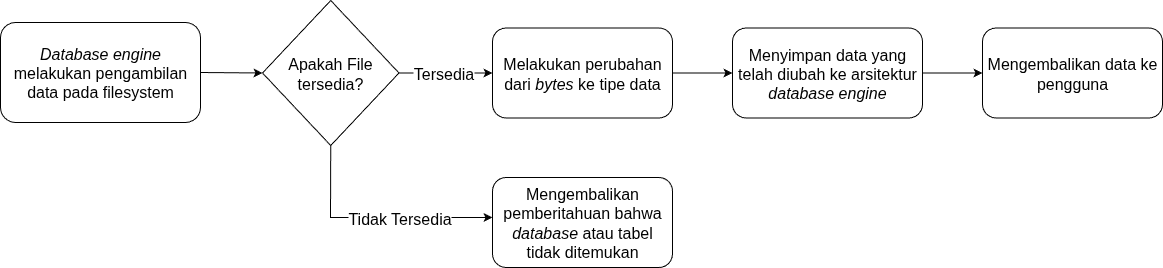
\includegraphics[width=0.9\textwidth]{gambar/bab3/proses-pengambilan-data-filesystem}
  \caption{Proses pengambilan data dari \emph{filesystem}}
\end{figure}

Pada bagian proses pembuatan dan penyimpanan data, memiliki alur yang sama dengan pengambilan data, namun terdapat proses tambahan,
yaitu data harus dikembalikan dalam bentuk \emph{bytes} dan disimpan di dalam \emph{filesystem}. Proses ini dimulai dari \emph{client} 
yang akan menjalankan proses \emph{insert} pada \emph{interface database}. \emph{Database engine} akan melakukan hal yang sama yaitu
pengambilan data, namun jika tabel yang dituju tidak tersedia maka akan mengembalikan sebuah pemberitahuan bahwa tabel tak bersedia. 
Setelah data berhasil diambil dari \emph{filesystem} dan disimpan ke dalam atribut, maka proses perubahan dari data ke \emph{bytes} akan dilakukan.
Data yang telah berubah menjadi \emph{bytes} akan disimpan ke dalam \emph{filesystem}. Berikut adalah alur dari proses penyimpanan jika data 
dalam atribut \emph{database} tersedia:


\begin{figure}[H]
  \centering{}
	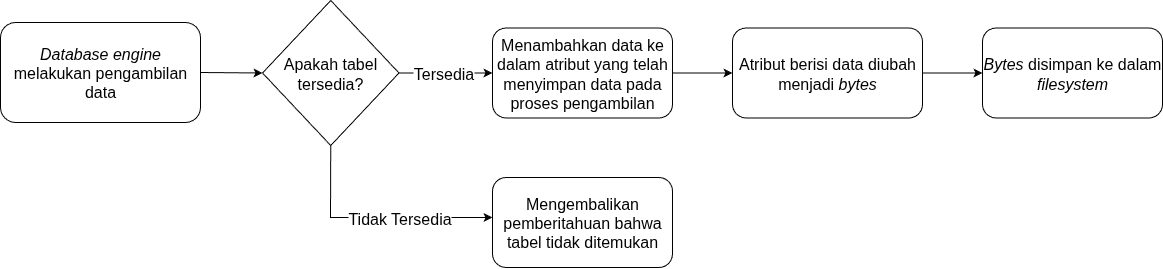
\includegraphics[width=0.9\textwidth]{gambar/bab3/proses-penyimpanan-data-filesystem}
  \caption{Proses penyimpanan data ke \emph{filesystem}}
\end{figure}

\section{\emph{Index} Sederhana dengan \emph{Map}}
Untuk proses \emph{indexing} pada \emph{database engine}, akan memanfaatkan struktur data bernama \emph{Map}. Struktur data \emph{map} yang digunakan mengikuti \emph{library} 
standar pada bahasa pemrograman yang akan digunakan. Dengan menggunakan \emph{map} yang ada dalam bahasa pemrograman, maka tidak perlu membuat struktur data khusus
untuk menerapkan \emph{index} pada \emph{database}. Karena menggunakan \emph{library} standar, struktur data ini juga akan memiliki \emph{function} yang dapat digunakan untuk mempermudah
proses pengembangan. Selain memiliki \emph{function-function} yang dapat digunakan, \emph{Map} yang tersedia pada \emph{library} standar bahasa pemrograman umumnya dapat 
menyimpan berbagai jenis tipe data. Penerapan \emph{Map} di arsitektur \emph{database engine} ini kemungkinan akan diterapkan dengan struktur data yang lain seperti \emph{array}.

\section{\emph{Join} Antar Tabel}
Sesuai dengan pernyataan pada batasan masalah, fitur \emph{join} yang ada pada \emph{database engine} awal ini adalah melakukan \emph{join} antar 2 tabel saja.
Prinsip \emph{join} yang digunakan sama seperti \emph{join} yang dilakukan pada \emph{database relational} lainnya, yaitu dengan menggunakan \emph{foreign key}.
Untuk menghubungkan kedua tabel dalam satu \emph{database}, maka terdapat satu kolom (biasanya berupa ID) dalam sebuah tabel yang nilai kolom dari tabel tersebut
merujuk ke tabel lain. Jika terdapat baris dengan nilai sama pada kolom yang telah ditentukan antar tabel, maka baris tersebut akan dianggap menjadi 1 baris.
Perlu diketahui bahwa fitur \emph{join} ini masih bersifat mirip seperti \emph{LEFT JOIN} yang ada di \emph{relational database} dan baru bisa dilakukan antar 2 tabel.


\section{Komunikasi Interface \emph{Database} dengan D-Bus}

Komunikasi dengan D-Bus akan menggunakan \emph{library} D-Bus yang tersedia pada bahasa pemrograman
yang digunakan. Pembuatan koneksi ini menggunakan bahasa pemrograman yang sama dengan bahasa pemrograman yang digunakan
dalam pengembangan \emph{database engine}. Namun, meski dibuat dengan satu bahasa pemrograman, koneksi D-Bus tetap bersifat universal (Dapat digunakan pada sistem lain). 
Sehingga jika \emph{client} menggunakan bahasa pemrograman lain, koneksi D-Bus tetap bisa terhubung satu sama lain. 

Koneksi pada D-bus ini akan dihubungkan melalui path yang nanti akan ditentukan
sebagai path dari jalur koneksi \emph{database engine}. \emph{Client} harus mendefinisikan \emph{path} yang sama dengan 
\emph{database engine} agar bisa terhubung. Dengan koneksi ini, pihak \emph{client} dapat menjalankan fungsi-fungsi 
\emph{database engine} berdasarkan\emph{interface} yang telah dibuka. \emph{Interface} yang dibuka hanyalah
interface yang dapat berguna bagi \emph{client} dan bukan \emph{interface} yang bersifat \emph{low-level}.



\section{Alat dan Bahan}

Untuk melaksanakan penelitian terdapat alat dan bahan yang dibutuhkan, di antaranya 
adalah:
\begin{itemize}
	\item {
    Laptop yang mempunyai spesifikasi untuk menjalankan bahasa pemrograman \emph{rust} dan \emph{python}. Versi bahasa
    pemrograman yang digunakan saat pengembangan adalah rust versi 1.84.1 dan python versi 3.10.12.
  }
	\item {
    Gemini AI dan ChatGPT sebagai alat untuk mencari ide dan \emph{brainstorm}.
  }
	\item {
    \emph{Visual Studi Code} sebagai \emph{Code Editor} beserta \emph{extension} \emph{rust analyzer}.
  }
	\item {
    Koneksi Internet.
  }
 
\end{itemize}


\section{Skema Uji}

Pengujian akan dilakukan dengan menjalankan servis \emph{Client} dan \emph{Database Engine}.
Untuk melakukan pengujian, servis \emph{Client} akan menyiapkan data \emph{Dummy} yang berasal \emph{Faker API}.
\emph{Faker API} merupakan sebuah alat yang dapat membuat berbagai macam jenis data sehingga akan cocok
untuk digunakan dalam melakukan pengujian. Data dari \emph{Faker API} tersebut akan disimpan 
menggunakan JSON yang nanti akan di \emph{import} ke dalam servis \emph{Client}. Lalu servis \emph{Client} 
yang akan mengirimkan \emph{data dummy} tersebut ke \emph{database engine} melalui koneksi D-Bus yang 
telah di \emph{expose}. \emph{Database engine} akan mengolah data yang telah dikirim, berdasarkan \emph{interface}  
yang telah di \emph{expose} pada D-Bus.
%!TEX root = ../main.tex
%-------------------------------------------------------------------------------
%                            	BAB IV
%               		IMPLEMENTASI DAN PENGUJIAN
%-------------------------------------------------------------------------------

\chapter{HASIL DAN PEMBAHASAN}

\section{Implementasi}

Terdapat perubahan pada \emph{interface} yang telah dibuat pada gambar 3.2. Perubahan serta fungsionalitas dari \emph{method} pada interface akan 
dijelaskan pada sub bab implementasi dibawah. Selain itu, terdapat perbedaan pada bahasa pemrograman yang di jelaskan pada gambar 3.2, bahasa pemrograman
yang digunakan dalam penelitian ini adalah bahasa \emph{low-level} bernama rust. Versi bahasa rust yang digunakan pada saat pengembangan adalah
rust dengan versi 1.84.1, namun untuk menjalankan hasil akhir dari \emph{database engine} ini, tidak perlu menginstall bahasa rust karena hasil akhir atau hasil build
dari bahasa rust merupakan \emph{file} \emph{bin} yang dapat langsung dijalankan.

\subsection{Bahasa Pemrograman Rust}
Rust merupakan salah satu bahasa pemrograman yang mempunyai tingkat kecepatan yang tinggi. Berdasarkan web resmi dari dokumentasi rust,
rust memiliki performa yang baik, ketahanan yang baik dan produktivitas yang baik (dokumentasi yang lengkap). Rust dapat digunakkan pada
teknologi \emph{low-level} seperti embedding system, web assembly, pembuatan command line dan lainnya. Berdasarkan paper \emph{Towards Understanding 
the Runtime Performance of Rust} \cite{yuchen2022}, kecepatan performa rust tidak jauh berbeda dengan bahasa pemrograman C. Dengan begitu rust 
menjadi salah satu bahasa tercepat untuk saat ini. Rust bukanlah bahasa pemrograman yang mengadopsi Object Oriented Programming sehingga 
tidak memiliki class. Namun terdapat alternatif dalam penggunaan \emph{class} yaitu struct. Agar penulisan lebih jelas dan mudah dipahami, istilah
class akan digunakan daripada istilah struct.

Dengan membuat menggunakan bahasa rust, hasil akhir dari pengembangan ini akan dilakukan sebuah proses yang bernama \emph{build}. Dari proses \emph{build} ini,
database akan berjalan. Jika sudah dalam bentuk hasil \emph{build}, maka sudah tidak perlu memasang bahasa rust pada komputer yang dituju karena hasil dari \emph{build}
merupakan \emph{file} yang dapat dijalankan secara langsung.

\subsection{Struktur Folder}
Struktur folder yang digunakan merupakan dasar struktur \emph{folder} dari rust. Dalam \emph{folder} src terdapat \emph{folder} \emph{database} yang berisi \emph{class} dan \emph{method}
yang akan digunakan dalam menjalankan \emph{database engine}. Terdapat 1 \emph{file} bernama playground.js hanya sebagai penyimpanan code saat pengembangan. 
dan tidak digunakan pada \emph{database engine}. Terdapat 3 \emph{folder} tambahan di bagian \emph{root} \emph{folder}, yaitu client-test (untuk menyimpan pengujian client),
schema (menyimpan \emph{file} \emph{database}) dan \emph{index} (untuk menyimpan \emph{index} yang terdapat pada database). Lalu di bagian \emph{root} \emph{folder} juga terdapat \emph{folder} test-data, dalam \emph{folder} ini
berguna untuk menyimpan data-data yang berguna untuk testing dan dokumentasi. Terdapat dapat beberapa \emph{file} seperti article.json, crawling.json, dan crawl\_information.json 
untuk menampung data pengujian sementara dan test.js yang hanya digunakan untuk membantu penulisan (Untuk memanfaatkan \emph{extension prettier} untuk
mempercantik dokumentasi hasil data, seperti pada gambar 4.19). Berikut adalah struktur \emph{folder} dari \emph{database engine}:

\begin{figure}[H]
  \centering{}
	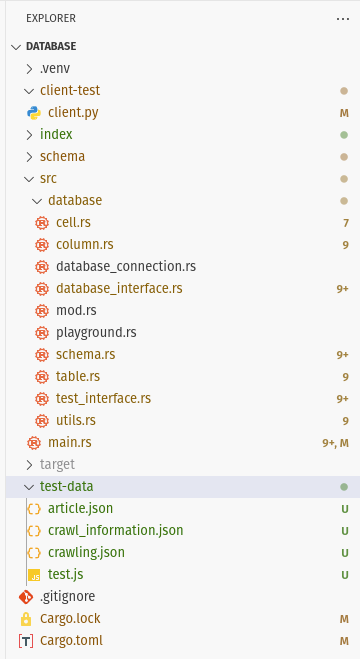
\includegraphics[width=0.3\textwidth]{gambar/bab4/struktur-folder.png}
  \caption{Struktur Folder}
\end{figure}


\subsection{Schema}
Class Schema merupakan \emph{class} induk pada \emph{database engine} yang dibuat. \emph{Class} ini menampung bagian penyimpanan data dan sebagai portal bagi pengolahan
data yang terjadi pada \emph{database engine}. \emph{Class} Schema ini akan merepresentasikan satu entitas \emph{database}. Berikut adalah \emph{class} diagram dari \emph{class} Schema.
\begin{figure}[H]
  \centering{}
	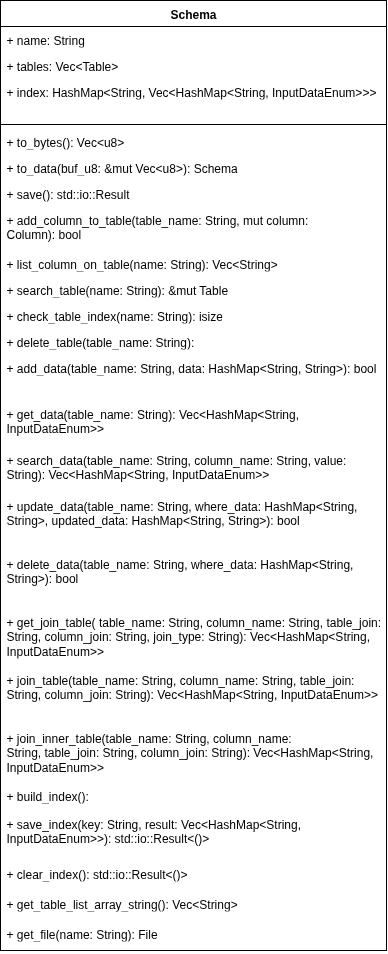
\includegraphics[width=0.3\textwidth]{gambar/bab4/Schema}
  \caption{Class Diagram Schema}
\end{figure}

Atribut dan \emph{method} yang tertulis pada \emph{class} diagram berguna untuk fitur yang ada di \emph{database} dan juga berguna saat pengembangan \emph{database engine}.
Terdapat 3 attribut pada \emph{class} Schema, yaitu:
\begin{enumerate}
	\item name \\
	Berguna untuk menyimpan nama dari \emph{database} dalam bentuk tipe data string.

	\item tables \\
	Attribut ini berguna untuk menyimpan list tabel yang ada pada \emph{database} atau schema yang dibuat. Tipe data atribut ini adalah Vector berisi \emph{class} table, yang akan 
  dijelaskan pada pembahasan \emph{class} berikutnya. 

	\item index  \\
	Atribut ini berguna untuk menyimpan \emph{index} yang ada pada instance schema yang dibuat. Tipe data dari atribut ini adalah HashMap, dan berisi
  struktur data yang cukup kompleks atau dalam. Hasmap pada atribut index ini memiliki key dengan tipe String, dan value sebuah vector. Vector didalamnya
  berisi beberapa HashMap yang nanti digunakan sebagai baris data yang telah disimpan. Lalu HashMap terdalam ini mempunyai key String dengan Value \emph{class} InputDataEnum.
			
\end{enumerate}

Untuk menggunakan dan mengolah data-data yang ada di dalam atribut, dibutuhkan method-method yang sudah dibuat dalam \emph{class} Schema. Terdapat 21 \emph{method} yang dapat digunakan, yaitu:

\begin{enumerate}
	\item to\_bytes \\
  \emph{Method} ini berguna untuk mengubah data yang telah disimpan pada atribut tabel. \emph{Method} ini mengembalikan sebuah vector yang berisi u8. Tipe u8 ini yang akan mempresentasikan 
  \emph{bytes} dan disimpan dalam \emph{filesystem}. Penyimpanan \emph{bytes} dalam vector memiliki urutan yang harus diperhatikan dan tidak boleh salah. Karena jika salah dapat menyebabkan data gagal
  diambil. Berikut adalah ilustrasi urutan dari penyimpanan \emph{byte} untuk \emph{class} Schema.

  \begin{figure}[H]
	\centering{}
		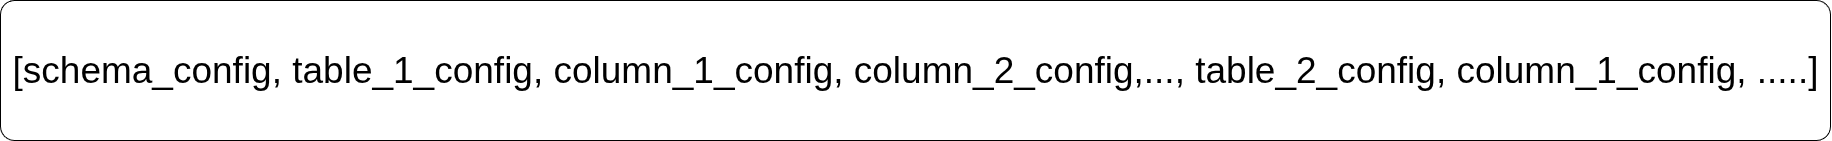
\includegraphics[width=0.9\textwidth]{gambar/bab4/urutan-penyimpanan-secara-keseluruhan.png}
	\caption{Urutan penyimpanan Schema secara menyeluruh dalam \emph{byte}}
	\end{figure}

	Untuk ilustrasi diatas, merupakan urutan penyimpanan data ke dalam bentuk \emph{byte} secara menyeluruh. \emph{schema\_config}, 
	\emph{table\_1\_config}, \emph{table\_2\_config}, \emph{column\_1\_config} dan lainnya merupakan urutan penyimpanan dari masing-masing class.
	Isi dari urutan penyimpanan tersebut akan dijelaskan di dalam \emph{method} to\_bytes pada masing-masing \emph{class}. Berikut ini merupakan isi urutan dari
	\emph{schema\_config}.

  \begin{figure}[H]
	\centering{}
		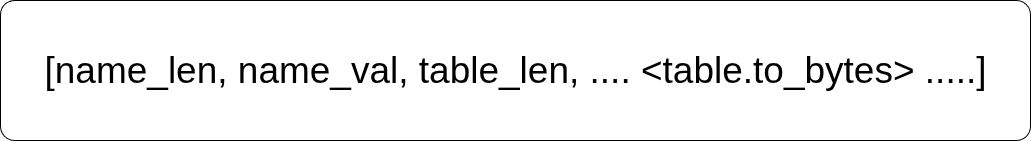
\includegraphics[width=0.6\textwidth]{gambar/bab4/urutan-penyimpanan-skema.png}
	\caption{Urutan penyimpanan Schema dalam \emph{byte}}
	\end{figure}


	\begin{enumerate}
		\item name\_len \\
		merupakan dari panjang atribut name yang disimpan dalam bentuk u8. \emph{Bytes} yang disimpan dibuat dengan panjang 8 mengikuti aturan primitif pada isize di bahasa pemrograman rust.
		
		\item name\_val \\
		merupakan value dari atribut name yang disimpan dalam bentuk u8. Panjang \emph{bytes} ini dapat berbeda-beda bergantung dengan isi dari nilainya. 

		\item table\_len \\
		merupakan dari panjang data tersimpan pada atribut tables yang disimpan dalam bentuk u8. Panjang penyimpanan juga mengikuti seperti apa yang telah di kutip di name\_len

		\item table.to\_bytes \\
		Urutan dilanjutkan memanggil \emph{method} to.bytes pada setiap data tersimpan pada atribut tables
	\end{enumerate}


	\item to\_data \\
	Method ini berguna untuk mengembalikan data yang telah disimpan pada \emph{method} to\_bytes dari bentuk vector u8 menjadi \emph{class} yang sebelumnya disimpan pada \emph{filesystem}. 
  Sehingga proses pengembaliannya merupakan kebalikan dari proses yang ada pada \emph{method} to\_bytes. \emph{Method} ini mengembalikan tipe data schema yang telah berisikan data. \emph{Method} ini bersifat
  static.

	\item save \\	
	Method ini digunakan untuk melakukan proses penyimpanan dari vector \emph{bytes} ke dalam \emph{filesystem}. Di dalam \emph{method} save, \emph{method} to\_bytes akan dipanggil dan return dari \emph{function} tersebut
  yang akan disimpan pada \emph{filesystem}. File disimpan ke dalam \emph{filesystem} dalam \emph{folder} schema, dan \emph{file} tersebut dinamakan dengan nama schema yang telah dibuat. \emph{Method} save ini nanti 
  juga akan selalu dipanggil setiap ada perubahan data seperti create, update dan juga delete untuk menunjang integritas data.

	\item add\_table \\
	Method yang berguna untuk menambah jumlah table yang disimpan pada \emph{class} Schema. Di dalam \emph{method} ini juga terdapat pengecekkan keunikan nama tabel. Jika terdapat tabel baru yang memiliki
  nama yang sama, maka \emph{method} ini akan mengembalikan error.

	\item add\_column\_to\_table \\
	Method yang berguna untuk menambahkan sebuah kolom baru pada tabel yang dituju.

	\item list\_column\_on\_table \\
	Method yang berguna untuk menampilkan kolom-kolom pada tabel yang dituju.
			

	\item search\_table \\
	Method yang berguna untuk mencari tabel yang terdapat dalam schema.

	\item check\_table\_index \\
	Method yang berguna untuk menampilkan \emph{index} atau urutan tabel di dalam vector table berdasarkan nama tabel pada \emph{parameter}.

	\item delete\_table \\
	Method yang berguna untuk menghapus tabel berdasarkan nama pada \emph{parameter}.
  
	\item add\_data \\
	Method yang berguna untuk menambah data baru berdasarkan tabel yang telah disimpan pada \emph{database}.
  
	\item get\_data \\
	Method yang berguna untuk menampilkan semua data yang telah tersimpan pada tabel yang dituju.

	\item search\_data \\
	Method yang berguna untuk menampilkan pencarian data berdasarkan kolom-kolom pada tabel yang dituju.

	\item update\_data \\
	Method yang berguna untuk mengubah data berdasarkan kondisi yang ada pada \emph{parameter}. Data yang diubah adalah data yang juga ditentukan 
  pada \emph{parameter}.

	\item delete\_data \\
	Method yang berguna untuk menghapus data berdasarkan kondisi yang ada pada \emph{parameter}.

	\item join\_table \\
	Berguna untuk melihat data antar tabel yang dihubungkan melalui kolom yang telah dibuat pada saat pembuatan tabel. \emph{Method} ini berguna sebagai
  pengondisian pemanggilan \emph{method} berdasarkan tipe \emph{join} yang tersedia pada \emph{database engine} ini yaitu \emph{inner} \emph{join}, \emph{left} \emph{join} dan \emph{right} \emph{join}.

	\item left\_right\_join\_table \\
	Method yang berguna untuk melakukan \emph{left} atau \emph{right} \emph{join}. Perbedaan proses dari \emph{left} dan \emph{right} \emph{join} terletak hanya pada \emph{parameter} dari \emph{method} ini.
  
	\item join\_inner\_table \\
	Method yang berguna untuk melakukan \emph{inner} \emph{join}.
  
	\item build\_index \\
	Method yang berguna untuk membangun \emph{index} berdasarkan data \emph{index} yang telah disimpan pada \emph{file} \emph{index}. \emph{Method} ini dipanggil di dalam \emph{method} to\_data.

	\item save\_index \\
	Method yang berguna untuk menyimpan \emph{index} ke dalam \emph{filesystem}. \emph{Index} ini disimpan ke \emph{file} didalam \emph{folder} \emph{index}. Nama dari \emph{file} tersebut juga akan
  disamakan dengan nama schema yang telah dibuat.

	\item clear\_index \\
	Method yang berguna untuk membersihkan  atau menghapus \emph{index} yang telah disimpan. \emph{Method} ini selalu dipanggil di dalam \emph{method} save.
  
	\item get\_file \\
	Sebuah \emph{method} yang bersifat private, berguna untuk mengembalikan Object File berdasarkan nama yang ada pada \emph{parameter}. 
  \emph{Method} ini di panggil di dalam \emph{method} build\_index.

	\item list\_all\_table \\
	Method yang berguna untuk menampilkan nama tabel yang tersimpan pada schema dalam bentuk vector string.

	\item print \\
	Method yang digunakan hanya pada saat pengembangan berlangsung, berguna untuk menampilkan data pada terminal tempat \emph{database engine} di jalankan.
\end{enumerate}

\subsection{Table}
Class Table merupakan \emph{class} yang merepresentasikan sebuah tabel dalam \emph{database}. Berikut adalah gambar \emph{class} diagram dari \emph{class} Table:
\begin{figure}[H]
  \centering{}
	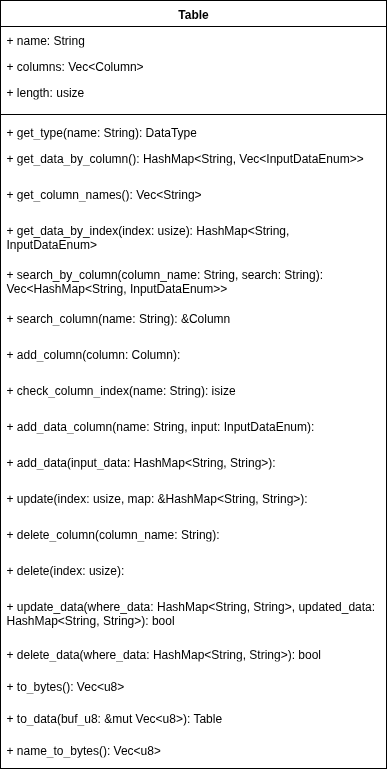
\includegraphics[width=0.6\textwidth]{gambar/bab4/Table}
  \caption{Class Diagram Table}
\end{figure}

Atribut dan \emph{method} yang tertulis pada \emph{class} diagram berguna untuk melakukan pengolahan data dari satu entitas Table. Sebagian besar dari atribut dan \emph{method} ini
dipanggil pada \emph{class} Schema. Terdapat 3 attribut pada \emph{class} Schema, yaitu:

\begin{enumerate}
	\item name \\
	Berguna untuk menyimpan nama dari tabel dalam bentuk tipe data string.

	\item columns \\
	Attribut ini berguna untuk menyimpan list kolom pada tabel yang dibuat. Tipe data atribut ini adalah Vector berisi \emph{class} Column, yang akan 
  dijelaskan pada pembahasan \emph{class} berikutnya. 

	\item length \\
	Berguna untuk menyimpan panjang dari vector columns. Atribut ini dapat dikatanak menyimpan panjang dari baris di tabel.
\end{enumerate}

Setelah atribut, terdapat method-method dalam \emph{class} Table yang berguna untuk mengolah data yang disimpan di dalam atribut. Terdapat 18 \emph{method} dalam \emph{class} Table, yaitu:

\begin{enumerate}
	\item get\_type \\
	Berguna untuk mengembalikan tipe data dari kolom yang dituju.

	\item get\_data\_by\_column \\
	Berguna untuk mengambalikan data-data yang tersimpan dalam kolom tabel dalam bentuk hashmap.

	\item get\_column\_names \\
	Berguna untuk melihat nama kolom yang tersimpan pada tabel dalam bentuk vector string.

	\item get\_data \\
	Berguna untuk mengambil seluruh data yang tersimpan pada satu \emph{class} Table.

	\item get\_data\_by\_index \\
	Method ini bersifat private, berguna untuk mengambil \emph{index} atau urutan data yang tersimpan pada tabel.

	\item search\_by\_column \\
	Method ini berguna untuk melakukan pencarian terhadap kolom yang dituju.

	\item search\_column \\
	Berguna untuk melakukan pencarian kolom berdasarkan nama kolom yang telah dibuat. 

	\item print \\
	Berfungsi sama seperti \emph{method} print yang ada pada \emph{class} Schema, berguna untuk menampilkan data yang tersimpan pada class
  Table di terminal tempat \emph{database engine} berjalan. \emph{Method} ini sering digunakan pada saat pengembangan saja.

	\item add\_column \\
	Berfungsi untuk menambah atau membuat kolom baru.

	\item check\_column\_index \\
	Berfungsi untuk mengembalikan \emph{index} atau urutan kolom yang tersimpan pada atribut columns.

	\item add\_data\_column \\
	Berfungsi untuk menambahkan 1 data pada suatu kolom, \emph{method} ini tidak digunakan dalam fitur \emph{database engine} ini karena dapat menghancurkan
  integritas antar kolom di sebuah tabel. Mungkin \emph{method} ini akan berguna di fitur yang akan datang.

	\item add\_data \\
	Berfungsi untuk menambahkan 1 baris data baru pada tabel.

	\item update \\
	Berfungsi untuk mengubah nilai atau isian pada 1 baris data yang dituju di sebuah tabel menggunakan \emph{index} atau urutan kolom pada tabel.

	\item delete\_column \\
	Berfungsi untuk menghapus kolom yang tersimpan pada tabel. Dengan menghapus kolom, maka semua data yang tersimpan pada kolom tersebut juga akan dihapus.
  Menggunakan nama kolom untuk mencari kolom yang dituju.

	\item delete \\
	Berfungsi untuk menghapus data pada tabel menggunakan \emph{index} atau urutan dari data yang telah tersimpan.
  
	\item update\_data \\
  Memiliki fungsi yang sama dengan \emph{method} update, namun menggunakan pencarian berdasarkan kolom-kolom yang ada pada tabel untuk mencari data yang ingin diubah.
  
	\item delete\_data \\
  Memiliki fungsi yang sama dengan \emph{method} delete, perbedaannya terletak pada pencariannya. \emph{Method} ini menggunakan kolom-kolom yang tersedia untuk menentukan
  baris data yang ingin dihapus.

	\item to\_bytes \\
  Memiliki fungsi yang sama dengan \emph{method} to\_bytes pada \emph{class} Schema, namun dikhususkan untuk mengubah \emph{class} Table saja. Proses pengubahan disimpan ke dalam vector
  u8 dengan urutan yang harus konsisten. Berikut adalah ilustrasi urutan penyimpanan dalam vector tersebut.

	\begin{figure}[H]
		\centering{}
			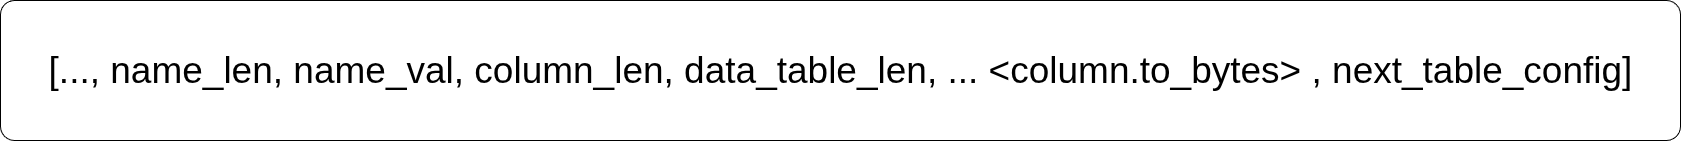
\includegraphics[width=0.6\textwidth]{gambar/bab4/urutan-penyimpanan-table.png}
		\caption{Urutan penyimpanan Table dalam byte}
		\end{figure}


	\begin{enumerate}
		\item name\_len \\
		merupakan dari panjang atribut name yang disimpan dalam bentuk u8. \emph{Bytes} yang disimpan dibuat dengan panjang 8 mengikuti aturan primitif pada isize di bahasa pemrograman rust.

		\item name\_val \\
		merupakan value dari atribut name yang disimpan dalam bentuk u8. Panjang \emph{bytes} ini dapat berbeda-beda bergantung dengan isi dari nilainya. 

		\item column\_len \\
		merupakan dari panjang data tersimpan pada atribut columns yang disimpan dalam bentuk u8. Panjang penyimpanan juga mengikuti seperti apa yang telah di kutip di name\_len

		\item data\_table\_len \\
		merupakan value dari atribut length yang disimpan dalam bentuk u8. Panjang \emph{bytes} ini juga mengikuti aturan pada name\_len. 

		\item column.to\_bytes \\
		Urutan dilanjutkan memanggil \emph{method} to.bytes pada setiap data tersimpan pada atribut columns

		\item \emph{next\_table\_config} \\
		Dilanjutkan dengan memanggil pengaturan tabel yang berikutnya.
	\end{enumerate}

	\item to\_data \\
  Proses yang berkebalikan dari \emph{method} to\_bytes, yaitu mengembalikan data dalam bentuk \emph{bytes} ke bentuk aslinya (class). Data yang dikembalikan dari \emph{method} ini 
  berupa \emph{class} Table.
  
	\item name\_to\_bytes \\
  \emph{Method} yang berfungsi untuk mengubah nama tabel ke dalam bentuk vector u8.
\end{enumerate}

\subsection{Column}
Class Column merupakan \emph{class} yang merepresentasikan sebuah kolom didalam sebuah tabel. Berikut adalah gambar \emph{class} diagram dari \emph{class} Column:
\begin{figure}[H]
  \centering{}
	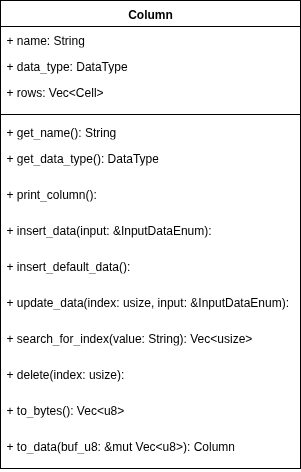
\includegraphics[width=0.6\textwidth]{gambar/bab4/Column}
  \caption{Class Diagram Column}
\end{figure}

Atribut dan \emph{method} yang tertulis pada \emph{class} diagram berguna untuk melakukan pengolahan data dari satu entitas Column. \emph{Class} Column dapat tersimpan dalam jumlah banyak di \emph{class} Table. 
Sebagian besar dari atribut dan \emph{method} ini juga akan dipanggil di \emph{class} Table. Terdapat 3 attribut pada \emph{class} Column, yaitu:

\begin{enumerate}
	\item name \\
	Berguna untuk menyimpan nama dari kolom dalam bentuk tipe data string.

	\item data\_type \\
	Attribut ini berguna untuk menyimpan tipe data dari sebuah kolom. Tipe data atribut ini adalah Enum DataType.

	\item rows \\
	Berguna untuk menyimpan data pada columns. Tipe data atribut rows meimiliki tipe vector yang berisi \emph{class} Cell.
\end{enumerate}

Selain atribut, \emph{class} Column ini juga memiliki \emph{method} yang berguna untuk mengolah data yang disimpan di atribut. Terdapat 10 \emph{method} di dalam \emph{class} Column, yaitu:

\begin{enumerate}
	\item get\_name \\
	Berguna untuk mengembalikan nama dari kolom.

	\item get\_data\_type \\
	Method yang berguna untuk mengembalikan tipe data dari data yang disimpan dalam \emph{class} Column.

	\item print\_column \\
	Method ini hanya dipakai pada saat pengembangan, dan memiliki fungsional yang sama seperti print \emph{method} di \emph{class} Schema dan \emph{class} Table. Berfungsi untuk menampilkan
  data yang disimpan pada terminal tempat \emph{database engine} dijalankan.

	\item insert\_data \\
	Method ini berguna untuk membuat data baru pada kolom. Data baru yang masuk ke dalam kolom harus disesuaikan dengan tipe data yang ada pada atribut data\_type.

	\item insert\_default\_data \\
	Method ini berguna untuk membuat data baru pada kolom dengan nilai default. String kosong untuk tipe data string dan nilai 0 untuk tipe data integer. Hal ini dibuat
  jika pengguna tidak mendefinisikan nilai pada kolom yang ada pada tabel saat menambahkan data baru.
  
	\item update\_data \\
	Berguna untuk mengubah data yang tersimpan pada atribut rows. \emph{Method} ini dipanggil di dalam \emph{method} update di \emph{class} Table.
  
	\item search\_for\_index \\
	Berguna untuk mengembalikan \emph{index} dari sebuah data yang tersimpan pada atribut rows. Rows yang dikembalikan adalah rows yang memiliki value yang ada di \emph{parameter}.
  \emph{Method} ini dapat mengembalikan indeks lebih dari 1 dalam bentuk vector.
  
	\item delete \\
	Berguna untuk menghapus data berdasarkan urutan atau indeks yang tersimpan pada atribut rows.
  
	\item to\_bytes \\
	Sama seperti \emph{method} di \emph{class} sebelumnya, berguna untuk mengubah data tersimpan ke dalam bentuk \emph{bytes} atau vector u8. Proses penyimpan ke dalam vector memiliki urutan
  yang harus sesuai. Berikut adalah ilustrasi urutan yang disimpan dalam vector.

  \begin{figure}[H]
	\centering{}
		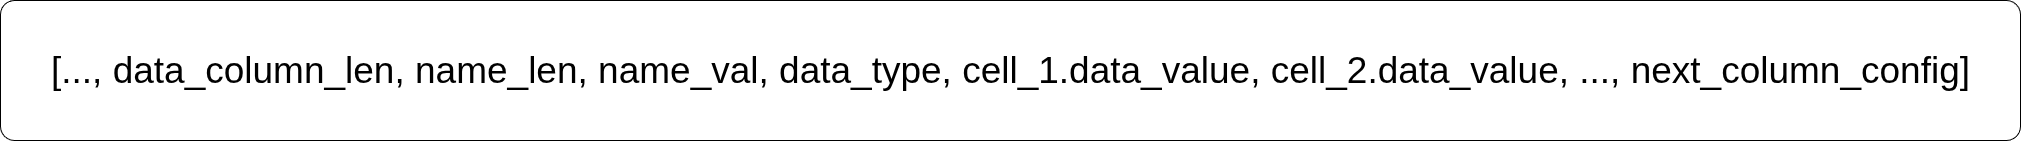
\includegraphics[width=0.8\textwidth]{gambar/bab4/urutan-penyimpanan-column.png}
	\caption{Urutan penyimpanan Column dalam byte}
	\end{figure}

	\begin{enumerate}
		\item data\_column\_len \\
		merupakan dari panjang data tersimpan pada atribut rows yang disimpan dalam bentuk u8. \emph{Bytes} yang disimpan dibuat dengan panjang 8 mengikuti aturan 
		primitif pada isize di bahasa pemrograman rust.

		\item name\_len \\
		merupakan dari panjang data dari atribut name yang disimpan dalam bentuk u8. Panjang penyimpanan juga mengikuti seperti apa yang telah di kutip di data\_column\_len

		\item name\_val \\
		merupakan value dari atribut name yang disimpan dalam bentuk u8. Panjang \emph{bytes} ini dapat berbeda-beda bergantung dengan isi dari nilainya. 

		\item data\_type \\
		Berguna untuk menyimpan tipe data dari kolom. Pada urutan ini jika bernilai 0 maka tipe data dari kolom nya adalah 0, dan jika bernilai 1 maka bernilai integer.


		\item cell.data\_value \\
		Urutan dilanjutkan dengan melakukan for loop dan memanggil atribut data\_value pada setiap cell yang disimpan di dalam atribut rows. Karena atribut data\_value sudah berupa vector u8 maka
		nilainya bisa langsung dimasukkan ke dalam vector. Namun terdapat sedikit perbedaan proses pada string, karena harus menambah panjang dari value string yang tersimpan terlebih dahulu
		sebelum menyimpan nilai aslinya. 

		\item \emph{next\_column\_config} \\
		Dilanjutkan dengan memanggil pengaturan kolom yang berikutnya.
	\end{enumerate}
  
	\item to\_data \\
	Berfungsi untuk mengembalikan data kolom yang telah diubah ke \emph{bytes} menjadi data \emph{class} Column kembali.
\end{enumerate}

\subsection{Cell}
Class Cell merupakan \emph{class} yang merepresentasikan sebuah nilai yang tersimpan pada satu baris tabel. \emph{Class} Cell dibutuhkan karena, setiap nilai yang tersimpan dalam database
dapat memiliki tipe data yang berbeda-beda. Sehingga diperlukan sebuah \emph{class} kembali untuk menentukan hal tersebut. Berikut adalah gambar \emph{class} diagram dari \emph{class} Cell:
\begin{figure}[H]
  \centering{}
	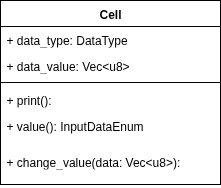
\includegraphics[width=0.6\textwidth]{gambar/bab4/Cell}
  \caption{Class Diagram Cell}
\end{figure}

Class Cell memiliki atribut dan beberapa \emph{method} yang berguna untuk menunjang fitur pada \emph{database engine}. Terdapat 2 attribut dalam \emph{class} Cell, yaitu:
\begin{enumerate}
	\item data\_type \\
	Berguna untuk menyimpan tipe data dari sebuah cell. Atribut ini memiliki tipe data Enum DataType dan berfungsi untuk memvalidasi tipe data yang ada pada cell
  dan \emph{class} Column tempat cell disimpan.  

	\item data\_value \\
	Berguna untuk menyimpan nilai atau value dari sebuah cell. Nilai atribut ini disimpan dalam bentuk vector u8. Tujuan dibuat seperti ini dikarenakan nilai yang disimpan
  dalam sebuah cell dapat memiliki tipe yang berbeda-beda.  Selain itu, dengan menggunakan vector u8 sebagai nilai dari atribut ini, proses penyimpanan ke \emph{filesystem} menjadi lebih
  karena dapat dilakukan tanpa perlu mengubahnya terlebih dahulu. 
\end{enumerate}

Atribut yang disimpan dalam sebuah Cell harus diolah agar dapat dikelola oleh \emph{database engine}. Dengan menggunakan method, kita dapat mengolah atribut agar dapat digunakan pada
fitur \emph{database engine}. Terdapat 3 \emph{method} yang terdapat pada \emph{class} Cell, yaitu:

\begin{enumerate}
	\item print \\
	Method yang berguna selama pengembangan \emph{database engine}. Berguna untuk menampilkan value dalam cell di terminal tempat \emph{database engine} dijalankan.  

	\item value \\
  Berguna untuk mengembalikan value dari bentuk \emph{byte} ke Enum InputDataEnum. Hal ini diperlukan karena nilai yang tersimpan dalam cell adalah \emph{bytes}, sehingga membutuhkan pemrosesan
  kembali ke tipe data asli nya. 

	\item change\_value \\
  Berguna untuk mengubah value yang tersimpan pada atribute data\_value sesuai dengan yang ada pada \emph{parameter}. Data dalam \emph{parameter} juga sudah dalam bentuk vector u8. 
\end{enumerate}

\subsection{Enumeration}
Terdapat beberapa nilai enum yang digunakan sebagai penyimpanan tipe data dalam \emph{database}. Terdapat 2 Enum class, yaitu:
\begin{enumerate}
	\item InputDataEnum \\
  Enum ini berguna untuk menyimpan data dalam bentuk String, Integer dan juga Null. Namun pada fitur \emph{database} kali ini, hanya 2 tipe data saja yang baru didukung untuk penyimpanannya
  yaitu String dan Integer. Khusus untuk enum ini, akan menggunakan library bernama serde dan serde\_derive untuk melakukan \emph{Serialization} dan \emph{Deserialization}. Hal ini diperlukan saat sedang
  melakukan penyimpanan \emph{index}, karena \emph{index} disimpan dalam bentuk HashMap. Dengan menggunakan library ini Hashmap yang berisi InputDataEnum dapat berubah ke dalam bentuk \emph{bytes} secara langsung
  tanpa perlu mengubahnya secara manual. Selain library serde dan serde\_derive, terdapat 1 macro lagi yang diterapkan pada enum ini yaitu Debug. Macro ini berguna agar value yang memiliki tipe InputDataEnum dapat
  dilihat hasilnya di terminal.
	
	\item DataType \\
  Enum yang berguna untuk menentukan tipe kolom yang tersimpan pada tabel dan tipe Cell yang tersimpan pada kolom.
\end{enumerate}

\subsection{Utils}
Selain beberapa \emph{class} inti, terdapat beberapa \emph{function} tambahan yang berguna untuk menunjang fitur-fitur yang tersedia pada \emph{database engine}. Semua \emph{function} ini tersimpan secara statis
pada \emph{file} utils.rs. Namun tidak semua \emph{function} dalam utils digunakan dalam penerapa fitur \emph{database engine}, sebagian hanya digunakan saat hendak melakukan debugging atau saat hendak melakukan
percobaan.

\subsection{DatabaseInterface}
Class \emph{DatabaseInterface} ini berfungsi sebagai penentu \emph{method} atau \emph{function} mana saja didalam \emph{database} yang dapat dijalankan oleh pengguna. Oleh karena itu, method-method di dalam class
ini hanya meneruskan paramater yang diterima ke \emph{method} yang ada dalam \emph{class} Schema sesuai dengan nama dari methodnya. Berikut adalah \emph{class} Diagram \emph{DatabaseInterface}.

\begin{figure}[H]
  \centering{}
	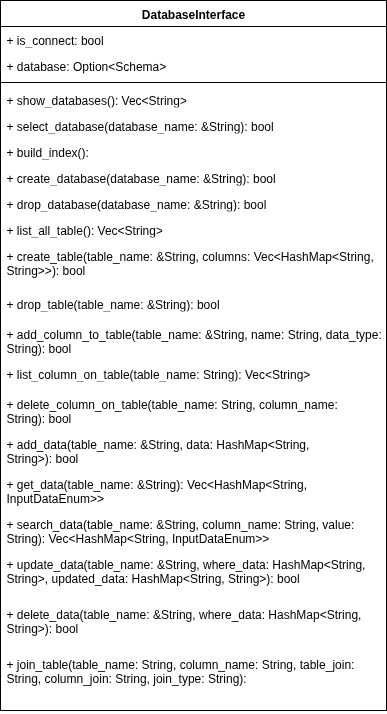
\includegraphics[width=0.6\textwidth]{gambar/bab4/DatabaseInterface.png}
  \caption{Class Diagram \emph{DatabaseInterface}}
\end{figure}

Perlu diperhatikan bahwa sebagian method-method di dalam \emph{class} ini, terutama
yang berhubungan dengan pengolahan data dalam database, memiliki validasi atau pengecekan apakah \emph{class} \emph{DatabaseInterface} sudah terhubung dengan \emph{class} Schema. \emph{Class} \emph{DatabaseInterface} ini memiliki
2 atribut yaitu:
\begin{enumerate}
	\item is\_connect \\
  Atribut dengan tipe data boolean untuk menentukan apakah instance schema sudah terhubung atau belum.
	
	\item database \\
  Atribut dengan tipe Option yang akan berisi instance dari \emph{class} Schema dan dapat berisi None jika instance Schema belum terhubung.
\end{enumerate}

Selain sebagai penentu method, terdapat mehod lain yang terdapat pada \emph{DatabaseInterface}. Berikut adalah method-method tambahan yang ada pada \emph{DatabaseInterface}:
\begin{enumerate}
	\item show\_databases \\
  \emph{Method} ini berguna untuk melihat list \emph{database} yang tersimpan dalam bentuk \emph{file} di \emph{folder} schema.

	\item select\_database \\
  \emph{Method} ini berguna untuk memilih \emph{database} dan memasukkannya ke dalam atribute \emph{database}.

	\item create\_database \\
  Berguna untuk membuat \emph{database} dan memanggil \emph{function} save di dalam \emph{class} Schema sehingga sebuah \emph{file} baru dibuat di dalam \emph{folder} schema sesuai dengan
  nama \emph{database} yang dimasukkan dalam \emph{parameter}.

	\item drop\_database \\
  Berguna untuk menghapus \emph{database} dengan cara menghapus \emph{file} \emph{database} pada \emph{folder} schema dan \emph{folder} \emph{index}.

	\item join\_data \\
	Terdapat sedikit perbedaan pada proses yang terjadi di dalam \emph{method} join\_data ini. Isi \emph{method} ini akan dijelaskan 
	lebih secara khusus pada sub bab 4.1.10 tentang \emph{indexing}
	
\end{enumerate}

\subsection{\emph{Indexing} pada fitur Join}
Penerapan fitur \emph{indexing} pada \emph{database engine} ini dilakukan pada fitur \emph{join}. Prinsip penerapannya sama seperti \emph{cache} pada umumnya. Hashmap digunakan
untuk mengumpulkan \emph{index} dengan menggunakan key dari \emph{parameter} yang dijalankan saat hendak menjalankan \emph{join}. Jika key dari \emph{parameter} tersedia dalam Hashmap, maka value dari
key tersebut akan dikembalikan. Sementara jika key tersebut tidak tersedia, maka akan memanggil \emph{method} join\_data yang ada pada \emph{class} Schema. Alur lebih detail terkait 
penerapan \emph{indexing} dapat dilihat pada \emph{method} join\_data pada \emph{class} \emph{DatabaseInterface}. Namun untuk penerapan \emph{indexing} saat ini masih belum berjalan dengan baik,
dikarenakan value disimpan dalam HashMap, dimana HashMap tersebut merupakan library bawaan dari rust. Value yang dikembalikan dari HashMap tersebut merupakan sebuah reference
dari value yang disimpan. Sementara nilai yang berupa reference tidak bisa di kembalikan atau di return dalam \emph{function} di bahasa pemrograman Rust. Untuk melakukan hal tersebut,
membutuhkan sebuah fitur yang bernama lifetime dan fitur lifetime ini masih belum bisa dikuasai penulis saat ini. Maka dari itu fitur join\_table bisa berjalan dan mengembalikan data
jika fitur \emph{indexing} ini dimatikan. Jika hanya ingin melihat isi data dari hasil \emph{indexing}, dapat menggunakan \emph{method} println! pada rust. Untuk penyimpanan \emph{HashMap} dalam \emph{filesystem}, 
akan menggunakan library bernama \emph{bincode}. Karena proses pengubahan dari data ke byte yang saat ini dibuat, hanya ditujukan
bagi \emph{class} schema, table dan column. 


\subsection{DatabaseConnection}
Class \emph{DatabaseConnection} merupakan \emph{class} yang berguna untuk \emph{database engine} melakukan koneksi ke sistem lain. \emph{Class} ini menggunakan 
DatabaseInterface sebagai penghubung ke \emph{class} Schema untuk menjalankan fungsi-fungsi \emph{database}. Seperti yang dikutip pada sub bab 3.7 bahwa untuk
melakukan koneksi eksternal dengan sistem lain, \emph{database engine} akan menggunakan D-Bus. Pada penelitian ini, penerapan D-Bus di \emph{database} akan menggunakan
library atau biasa disebut crates dalam bahasa rust. Crates tersebut bernama zbus. Untuk menggunakan zbus pada \emph{class} \emph{DatabaseConnection}, penerapan macro
interface diperlukan. Hal ini sesuai dengan petunjuk yang ada pada dokumentasi zbus. Lalu \emph{library} bernama tokio akan digunakan
untuk membuat \emph{connection} menggunakan zbus pada function main di \emph{file} main.rs. Berikut adalah \emph{class} diagram dari \emph{class} \emph{DatabaseConnection}.


\begin{figure}[H]
  \centering{}
	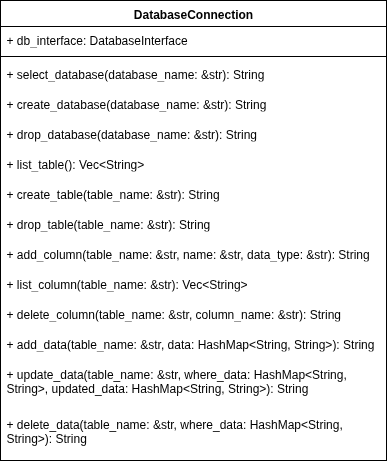
\includegraphics[width=0.6\textwidth]{gambar/bab4/DatabaseConnection}
  \caption{Class Diagram Column}
\end{figure}

Class \emph{DatabaseConnection} memiliki sebuah atribut bernama db\_interface. Atribut ini memiliki tipe data dari class
DatabaseInterface, yang berguna untuk memastikan bahwa \emph{class} \emph{DatabaseConnection} sudah terhubung dengan \emph{class} Schema.
Karena pada saat pertama kali \emph{database engine} ini dinyalakan, \emph{database} atau schema harus dipilih terlebih dahulu untuk
menentukan di schema mana data akan diolah. Untuk memilih schema, dapat menggunakan \emph{method} select\_database yang terdapat
pada \emph{class} \emph{DatabaseInterface}.

Perlu diketahui bahwa koneksi dengan menggunakan D-Bus untuk \emph{database engine} saat belum mendukung semua fungsi-fungsi pada \emph{database}. Karena secara default, 
koneksi dengan D-Bus hanya mendukung beberapa tipe data yang ada pada Rust saja. Untuk tipe data \emph{class} yang dibuat sendiri, diperlukan pengaturan tambahan agar bisa
melakukan koneksi ke sistem lain. Diantara \emph{method} yang mengembalikan tipe \emph{class} pada \emph{class} \emph{DatabaseInterface} adalah get\_data, search\_data, dan join\_table.
Oleh karena itu implementasi ketiga \emph{method} tersebut masih belum didukung pada koneksi melalui D-Bus saat ini.

\section{Pengujian}

Untuk pengujian akan dilakukan dengan 2 skema, yaitu pengujian secara  menggunakan bahasa pemrograman yang sama 
(dalam penelitian ini menggunakan bahasa rust) dan pengujian secara eksternal dengan menggunakan D-Bus yang akan digunakan pengguna
untuk menjalankan fungsi \emph{database}. Pengujian terpisah ini dilakukan berdasarkan alasan yang terdapat pada sub bab 4.1.11, yaitu tidak semua \emph{method} di 
DatabaseInterface dapat diakses oleh pengguna melalui D-Bus. 

Untuk memudahkan dalam pelaksanaan ujian, pada \emph{file} main.rs sebuah \emph{function} baru akan dibuat untuk
masing pengujian internal dan pengujian internal dengan data hasil \emph{crawling}. \emph{Function} untuk pengujian internal bernama test dan \emph{function} untuk pengujian internal
dengan data dummy bernama test\_data\_crawling. Masing-masing \emph{function} tersebut akan menerapkan \emph{macro} bernama \emph{test}. \emph{Macro} ini merupakan \emph{macro}
bawaan dari \emph{rust}. Lalu untuk \emph{function} main dalam main.rs, akan berisi konfigurasi untuk menjalankan \emph{library} zbus untuk menerima koneksi dari luar.

\subsection{Pengujian Internal}
Pengujian internal dilakukan dengan membuat sebuah \emph{class} baru bernama TestDatabaseInterface. Karena pengujian dilakukan  maka \emph{method} print 
pada setiap \emph{class} yang telah dijelaskan di sub bab sebelumnya, akan digunakan. Pengujian akan dilakukan dengan menggunakan data \emph{Dummy} yang terdiri dari 
2 tabel yang saling berkaitan. Berikut adalah isi tabel dari data \emph{Dummy} yang digunakan. 

\begin{table}[H]
  \centering{}
  \begin{tabular}{|m{2.5cm}|m{4cm}|m{4cm}|}
      \hline
      \textbf{id (Integer)} & \textbf{first\_name (String)} &  \textbf{last\_name (String)} \\
      \hline
      0 & Farhan & Abdul \\
      \hline
      1 & Akbar & Maulana \\
      \hline
      2 & Daffa & Haryadi \\
      \hline
      3 & Hanif & Ramadhan \\
      \hline
      4 & Rudiansyah & Wijaya \\
      \hline
  \end{tabular}
  \caption{Tabel Users}
\end{table}


\begin{table}[H]
  \centering{}
  \begin{tabular}{|m{2cm}|m{2cm}|m{3cm}|m{3cm}|}
      \hline
      \textbf{id (Integer)} & \textbf{user\_id (Integer)} & \textbf{title (String)} &  \textbf{description (String)} \\
      \hline
      0 & 0 & Judul 0 & \emph{Long Text} \\ 
      \hline
      1 & 0 & Judul 1 & \emph{Long Text} \\ 
      \hline
      2 & 1 & Judul 2 & \emph{Long Text} \\ 
      \hline
      3 & 2 & Judul 3 & \emph{Long Text} \\ 
      \hline
      4 & 2 & Judul 4 & \emph{Long Text} \\ 
      \hline
      5 & 2 & Judul 5 & \emph{Long Text} \\ 
      \hline
      6 & 3 & Judul 6 & \emph{Long Text} \\ 
      \hline
      7 & 2 & Judul 7 & \emph{Long Text} \\ 
      \hline
      8 & 2 & Judul 8 & \emph{Long Text} \\ 
      \hline
      9 & 2 & Judul 9 & \emph{Long Text} \\ 
      \hline
      10 & 1 & Judul 10 & \emph{Long Text} \\ 
      \hline
      11 & 1 & Judul 11 & \emph{Long Text} \\ 
      \hline
      12 & 2 & Judul 12 & \emph{Long Text} \\ 
      \hline
  \end{tabular}
  \caption{Tabel Posts}
\end{table}

Pada tabel posts, data yang digunakan pada kolom description akan diambil Faker API (\cite{faker}) supaya dapat berisi text yang panjang.
Lalu untuk kolom user\_id pada tabel posts, berguna untuk menghubungkan antara tabel posts dengan tabel users.
Pengujian dilakukan pada masing-masing \emph{method} yang ada pada \emph{class} \emph{DatabaseInterface}. Berikut adalah \emph{class} diagram
dari \emph{class} \emph{TestDatabaseInterface}.

\begin{figure}[H]
  \centering{}
	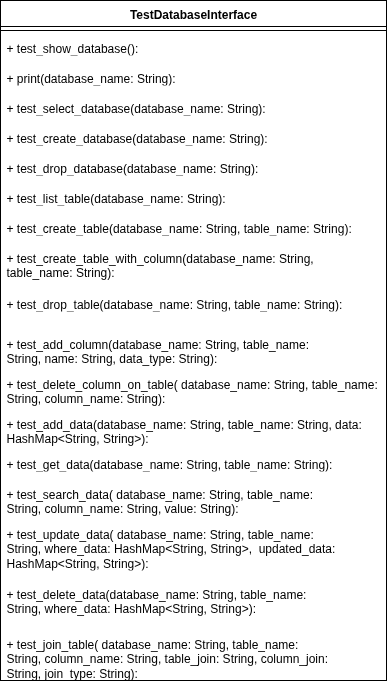
\includegraphics[width=0.6\textwidth]{gambar/bab4/TestDatabaseInterface.png}
  \caption{Class Diagram \emph{TestDatabaseInterface}}
\end{figure}

Pada penulisan ini pengujian akan berfokus pada fungsinal dasar \emph{database} yaitu membuat, melihat, mengubah dan menghapus data (CRUD).
Perlu diketahui bahwa pengujian yang dilakukan pada masing-masing \emph{function} dibuat dengan isian data yang sama satu sama lain. Lalu
terdapat sebuah informasi "Database berhasil terhubung" saat proses pengujian dibawah, dikarenakan proses \emph{database} harus terhubung terlebih dahulu
jika ingin menjalankan fungsinya. Jika terdapat tambahan seperti boolean true, juga penanda bahwa proses berhasil dijalankan.
Berikut ini adalah hasil pengujian database:

\begin{enumerate}
	\item test\_create\_database \\
  Pengujian dimulai dari mencoba melakukan pembuatan \emph{database}. \emph{Database} akan dibuat dengan nama articles. Dengan menjalankan \emph{function} ini
  maka akan terlihat sebuah \emph{file} baru dalam \emph{folder} schema dan \emph{folder} \emph{index}. File tersebut memiliki nama yang sama dengan \emph{database} yang dibuat.
  Pada terminal juga terdapat sebuah informasi bahwa \emph{database} berhasil terbuat.
  \begin{figure}[H]
  	\centering{}
	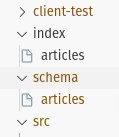
\includegraphics[width=0.3\textwidth]{gambar/bab4/test-create-database}
  	\caption{File baru telah terbuat dalam \emph{folder} \emph{index} dan schema}
  \end{figure}
	
	\item test\_select\_database \\
  \emph{Method} yang berguna untuk memilih \emph{database} terlebih dahulu. Karena tanpa melakukan pemilihan database, maka \emph{database engine} tidak akan berjalan.
  \emph{Database} yang dipilih adalah \emph{database} yang telah dibuat sebelumnya yaitu article. Jika pengujian ini berhasil maka akan muncul informasi bahwa
  \emph{database} berhasil terhubung.
   \begin{figure}[H]
  	\centering{}
	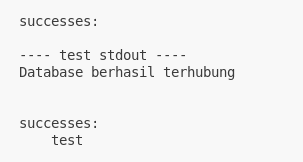
\includegraphics[width=0.6\textwidth]{gambar/bab4/test-select-database}
  	\caption{Informasi \emph{database} telah terhubung}
   \end{figure}

	\item test\_create\_table \\
  \emph{Method} yang berguna untuk membuat tabel pada \emph{database} yang dituju. Untuk kasus pengujian ini, vector kosong akan digunakan sebagai input dari kolom nya.
  Sehingga tabel yang terbuat adalah sebuah tabel tanpa kolom. \emph{Method} ini akan dijalankan 2x untuk menyesuaikan dengan data \emph{Dummy} yang terdapat pada tabel 4.1
  dan tabel 4.2. Nilai true pada gambar mengindikasikan bahwa pembuatan tabel telah berhasil.
  \begin{figure}[H]
  	\centering{}
	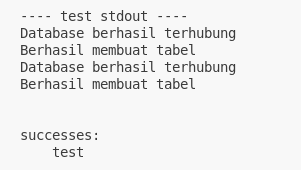
\includegraphics[width=0.6\textwidth]{gambar/bab4/test-create-table}
  	\caption{Informasi tabel telah berhasil terbuat}
   \end{figure}

	\item test\_add\_column \\
  Pengujian yang dilakukan untuk menambah kolom baru pada tabel yang telah dibuat. Kolom-kolom akan ditambahkan sesuai dengan nama dan tipe data yang ada pada tabel 4.1 dan tabel 4.2. 
  Oleh karena itu pengujian akan dilakukan sebanyak 7 kali menyesuaikan dengan jumlah kolom pada tabel yang disebutkan sebelumnya.
  \begin{figure}[H]
  	\centering{}
	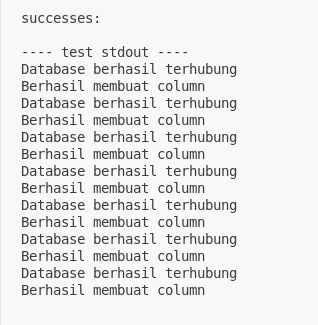
\includegraphics[width=0.3\textwidth]{gambar/bab4/test-create-column}
  	\caption{Informasi kolom telah berhasil terbuat}
   \end{figure}

	\item test\_add\_data \\
  Setelah berhasil membuat kolom, maka pengujian pembuatan dapat dilakukan. \emph{Method} pengujian ini akan membuat sebuah baris data baru di tabel dan kolom yang sudah dibuat. Jumlah dan 
  isian yang dibuat akan sama seperti data pada tabel 4.1 dan tabel 4.2.
  \begin{figure}[H]
  	\centering{}
	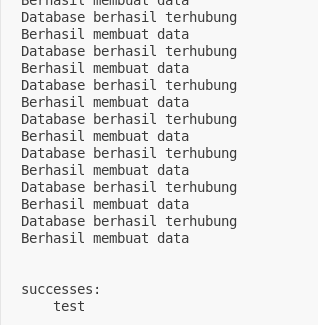
\includegraphics[width=0.4\textwidth]{gambar/bab4/test-create-data}
  	\caption{Informasi data telah berhasil terbuat}
   \end{figure}

	\item test\_get\_data \\
  Setelah berhasil membuat data, data yang telah disimpan akan diuji untuk proses pengambilannya. \emph{Method} ini akan menampilkan semua data pada tabel yang dituju dengan
  menggunakan \emph{method} print di dalam \emph{class} Table.
  \begin{figure}[H]
  	\centering{}
	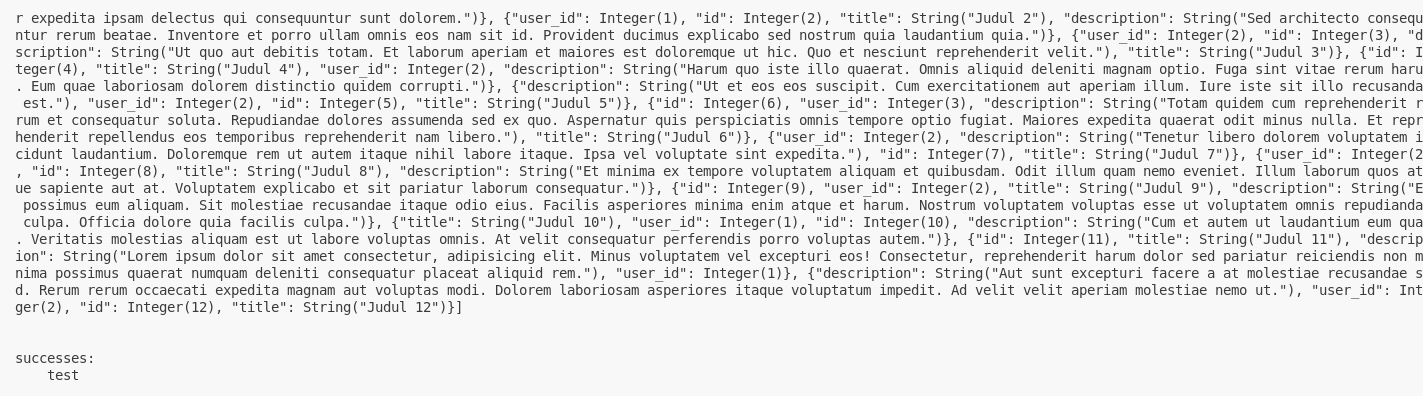
\includegraphics[width=0.6\textwidth]{gambar/bab4/test-get-data-posts.png}
  	\caption{Hasil data tabel \emph{posts} telah berhasil terbuat}
   \end{figure}
  \begin{figure}[H]
  	\centering{}
	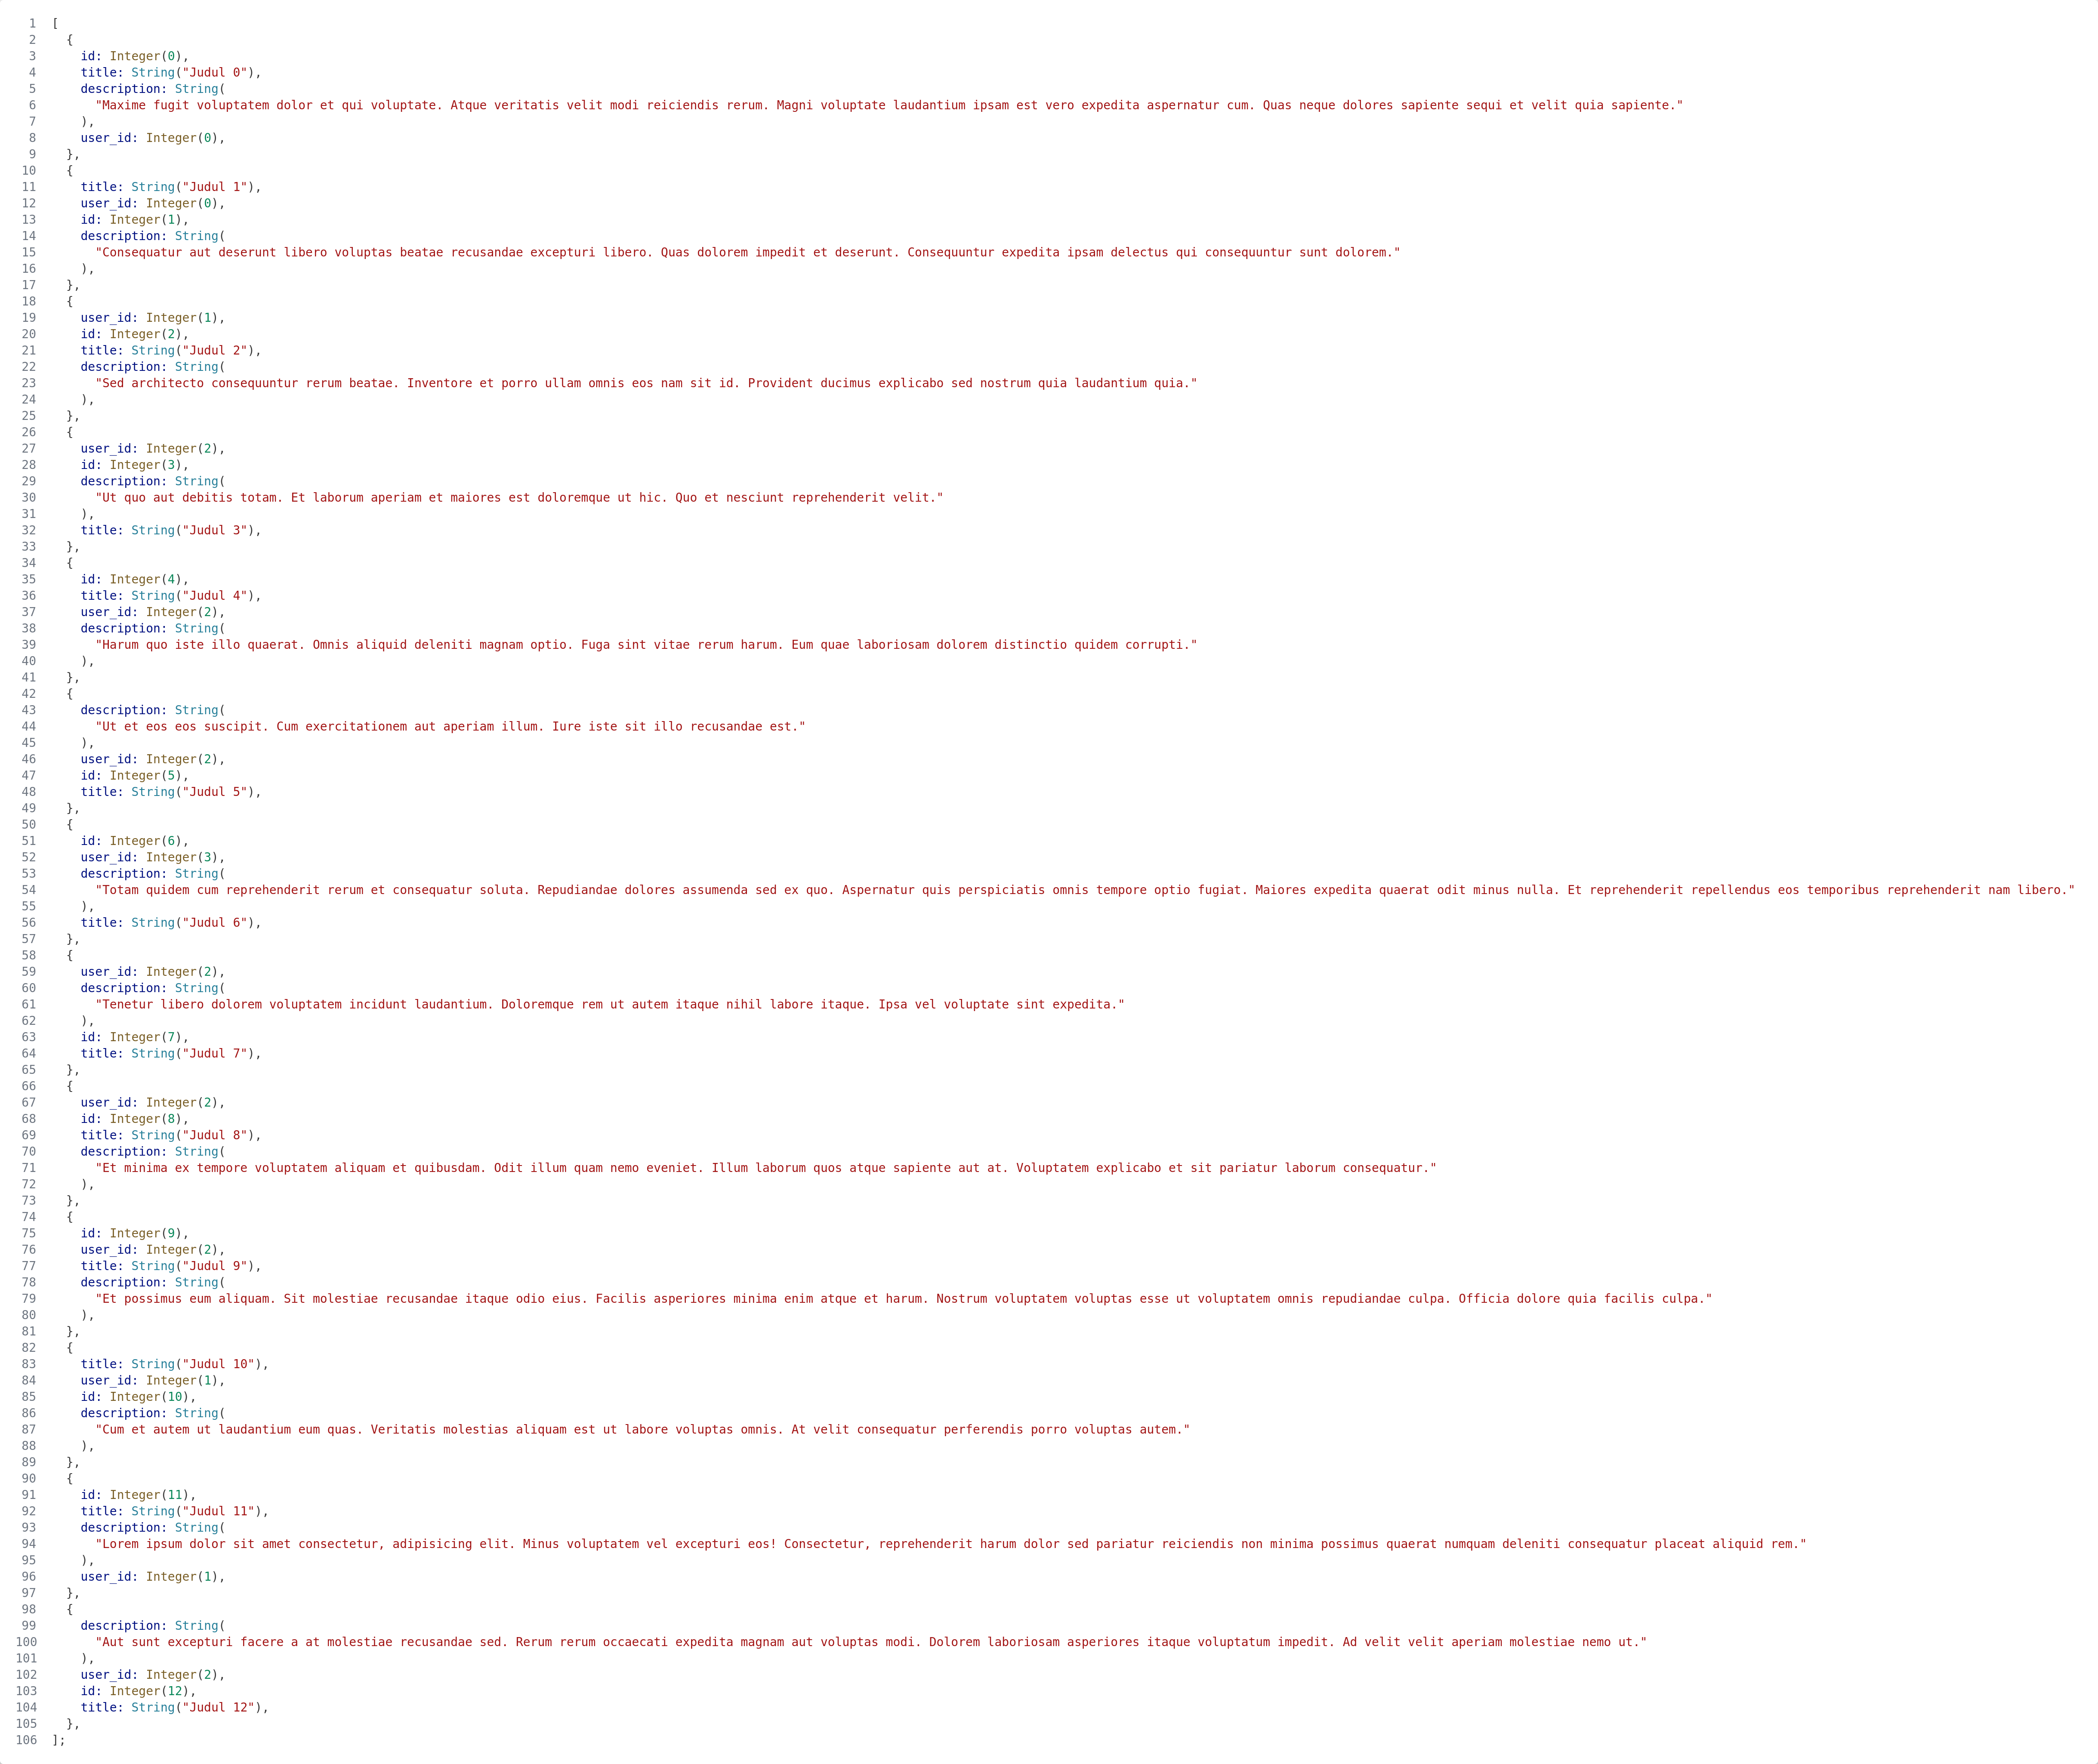
\includegraphics[width=0.9\textwidth]{gambar/bab4/test-get-data-posts-beautify.png}
  	\caption{Hasil data tabel \emph{posts} yang telah diformat menggunakan \emph{prettier} (\emph{Extension} \emph{Visual Studio Code} pada Javascript)}
   \end{figure}

  \begin{figure}[H]
  	\centering{}
	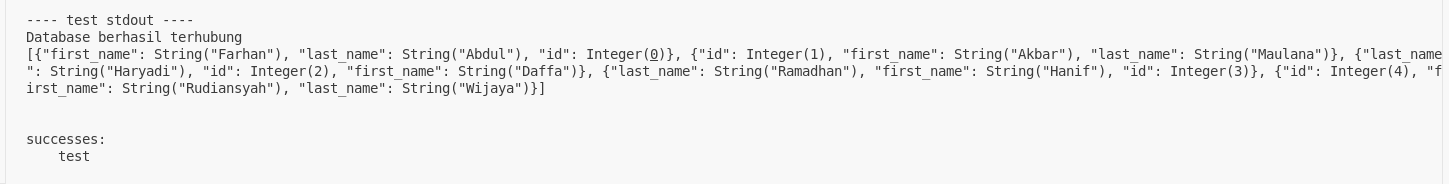
\includegraphics[width=0.6\textwidth]{gambar/bab4/test-get-data-users.png}
  	\caption{Hasil data tabel \emph{users} telah berhasil terbuat}
   \end{figure}
  \begin{figure}[H]
  	\centering{}
	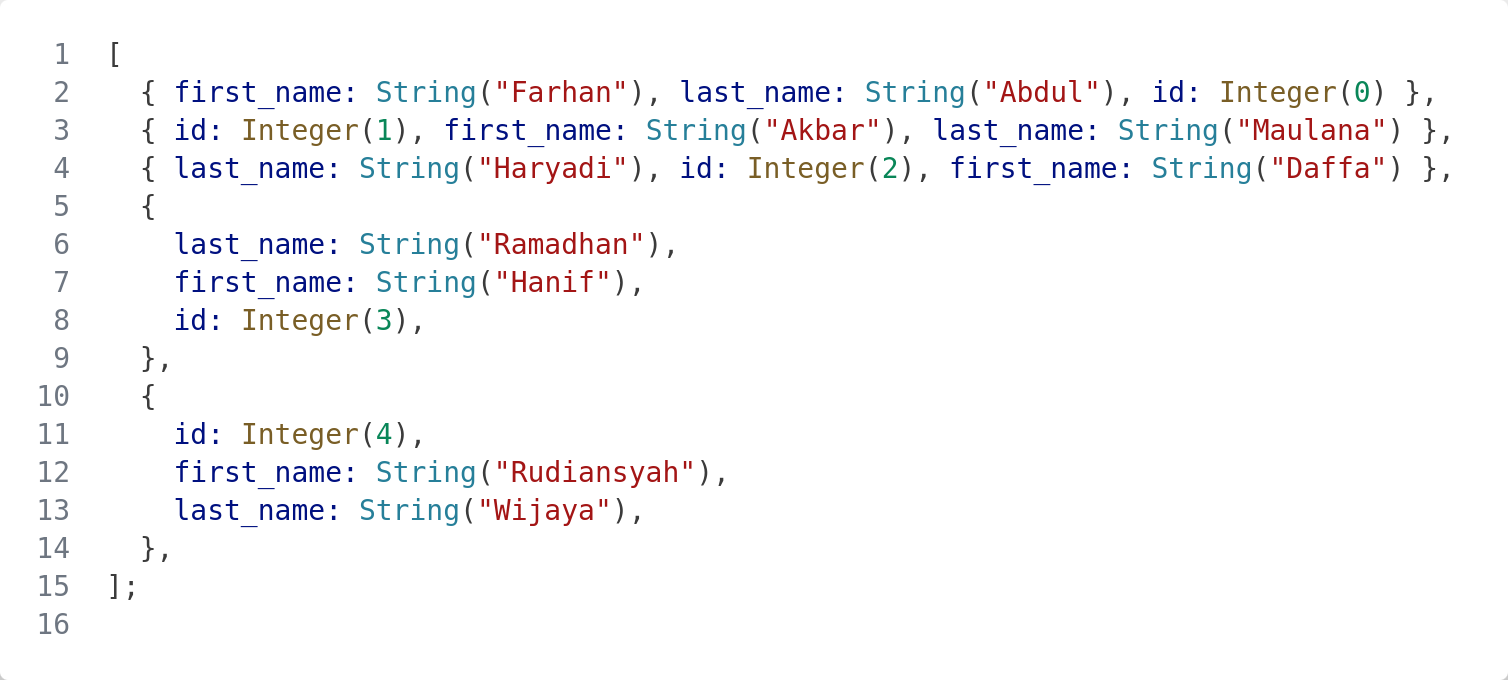
\includegraphics[width=0.9\textwidth]{gambar/bab4/test-get-data-users-beautify.png}
  	\caption{Hasil data tabel \emph{users} yang telah diformat menggunakan \emph{prettier} (\emph{Extension} \emph{Visual Studio Code} pada Javascript)}
   \end{figure}

	\item test\_update\_data \\
  \emph{Method} pengujian ini akan melakukan pengubahan pada data yang telah disimpan di \emph{database}. Pengujian ini membutuhkan \emph{parameter} untuk menentukan data mana yang akan dihapus, dan data apa saja
  yang akan diubah. Untuk kasus uji kali ini, akan mengubah kolom pada tabel users yang memiliki id dengan value 0 dan first\_name yang memiliki value "Farhan". Sementara data yang diubah adalah
  kolom last\_name, yang akan diubah berisi "Abdul Hamid".

  \begin{figure}[H]
  	\centering{}
	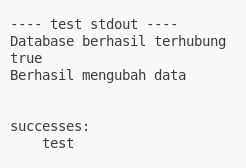
\includegraphics[width=0.6\textwidth]{gambar/bab4/test-update-data.png}
  	\caption{Informasi data berhasil diubah}
   \end{figure}

	\item test\_search\_data \\
  Pengujian \emph{method} search data ini dilakukan dengan memasukkan kolom dan value yang dituju. Data yang dicari adalah data pada tabel users yang memiliki id 0.
  \begin{figure}[H]
  	\centering{}
	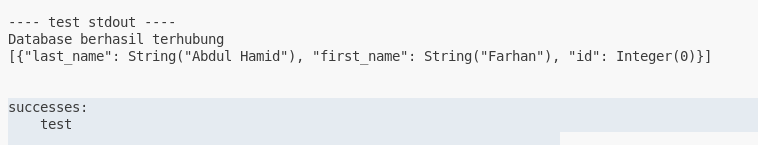
\includegraphics[width=0.6\textwidth]{gambar/bab4/test-search-data-users.png}
  	\caption{Informasi hasil pencarian}
   \end{figure}
    \begin{figure}[H]
  	\centering{}
	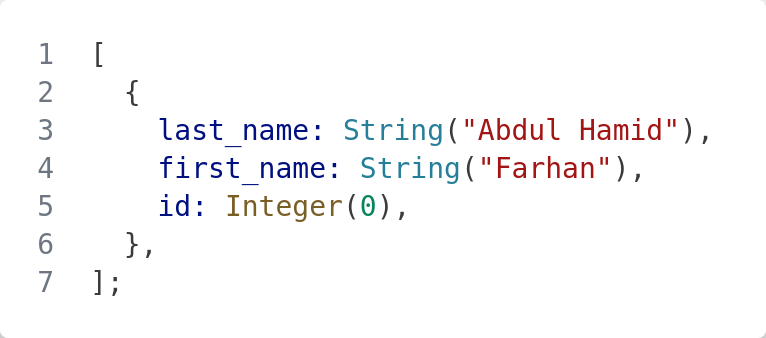
\includegraphics[width=0.7\textwidth]{gambar/bab4/test-search-data-users-beautify.png}
  	\caption{Hasil data yang telah diformat menggunakan \emph{prettier} (\emph{Extension} VSCode pada Javascript)}
   \end{figure}
  
  \item test\_join\_data \\
  Untuk menjalankan pengujian ini, kolom user\_id pada tabel posts akan digunakan untuk menyocokan data ke tabel users. Tabel, kolom serta tipe \emph{join} harus
  didefinisikan untuk menjalankan pengujian \emph{join} ini. Pada saat melakukan pengujian ini, terdapat beberapa error yang dialami dikarenakan \emph{index} yang tidak valid
  serta kesalahan dalam pengondisian \emph{join} nya. Namun untuk gambar dibawah, merupakan hasil dari implementasi yang telah diperbaiki.
  \begin{figure}[H]
  	\centering{}
	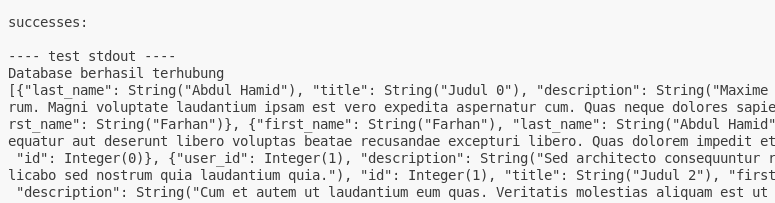
\includegraphics[width=0.6\textwidth]{gambar/bab4/test-join-data-inner.png}
  	\caption{Informasi hasil \emph{inner join}}
   \end{figure}
    \begin{figure}[H]
  	\centering{}
	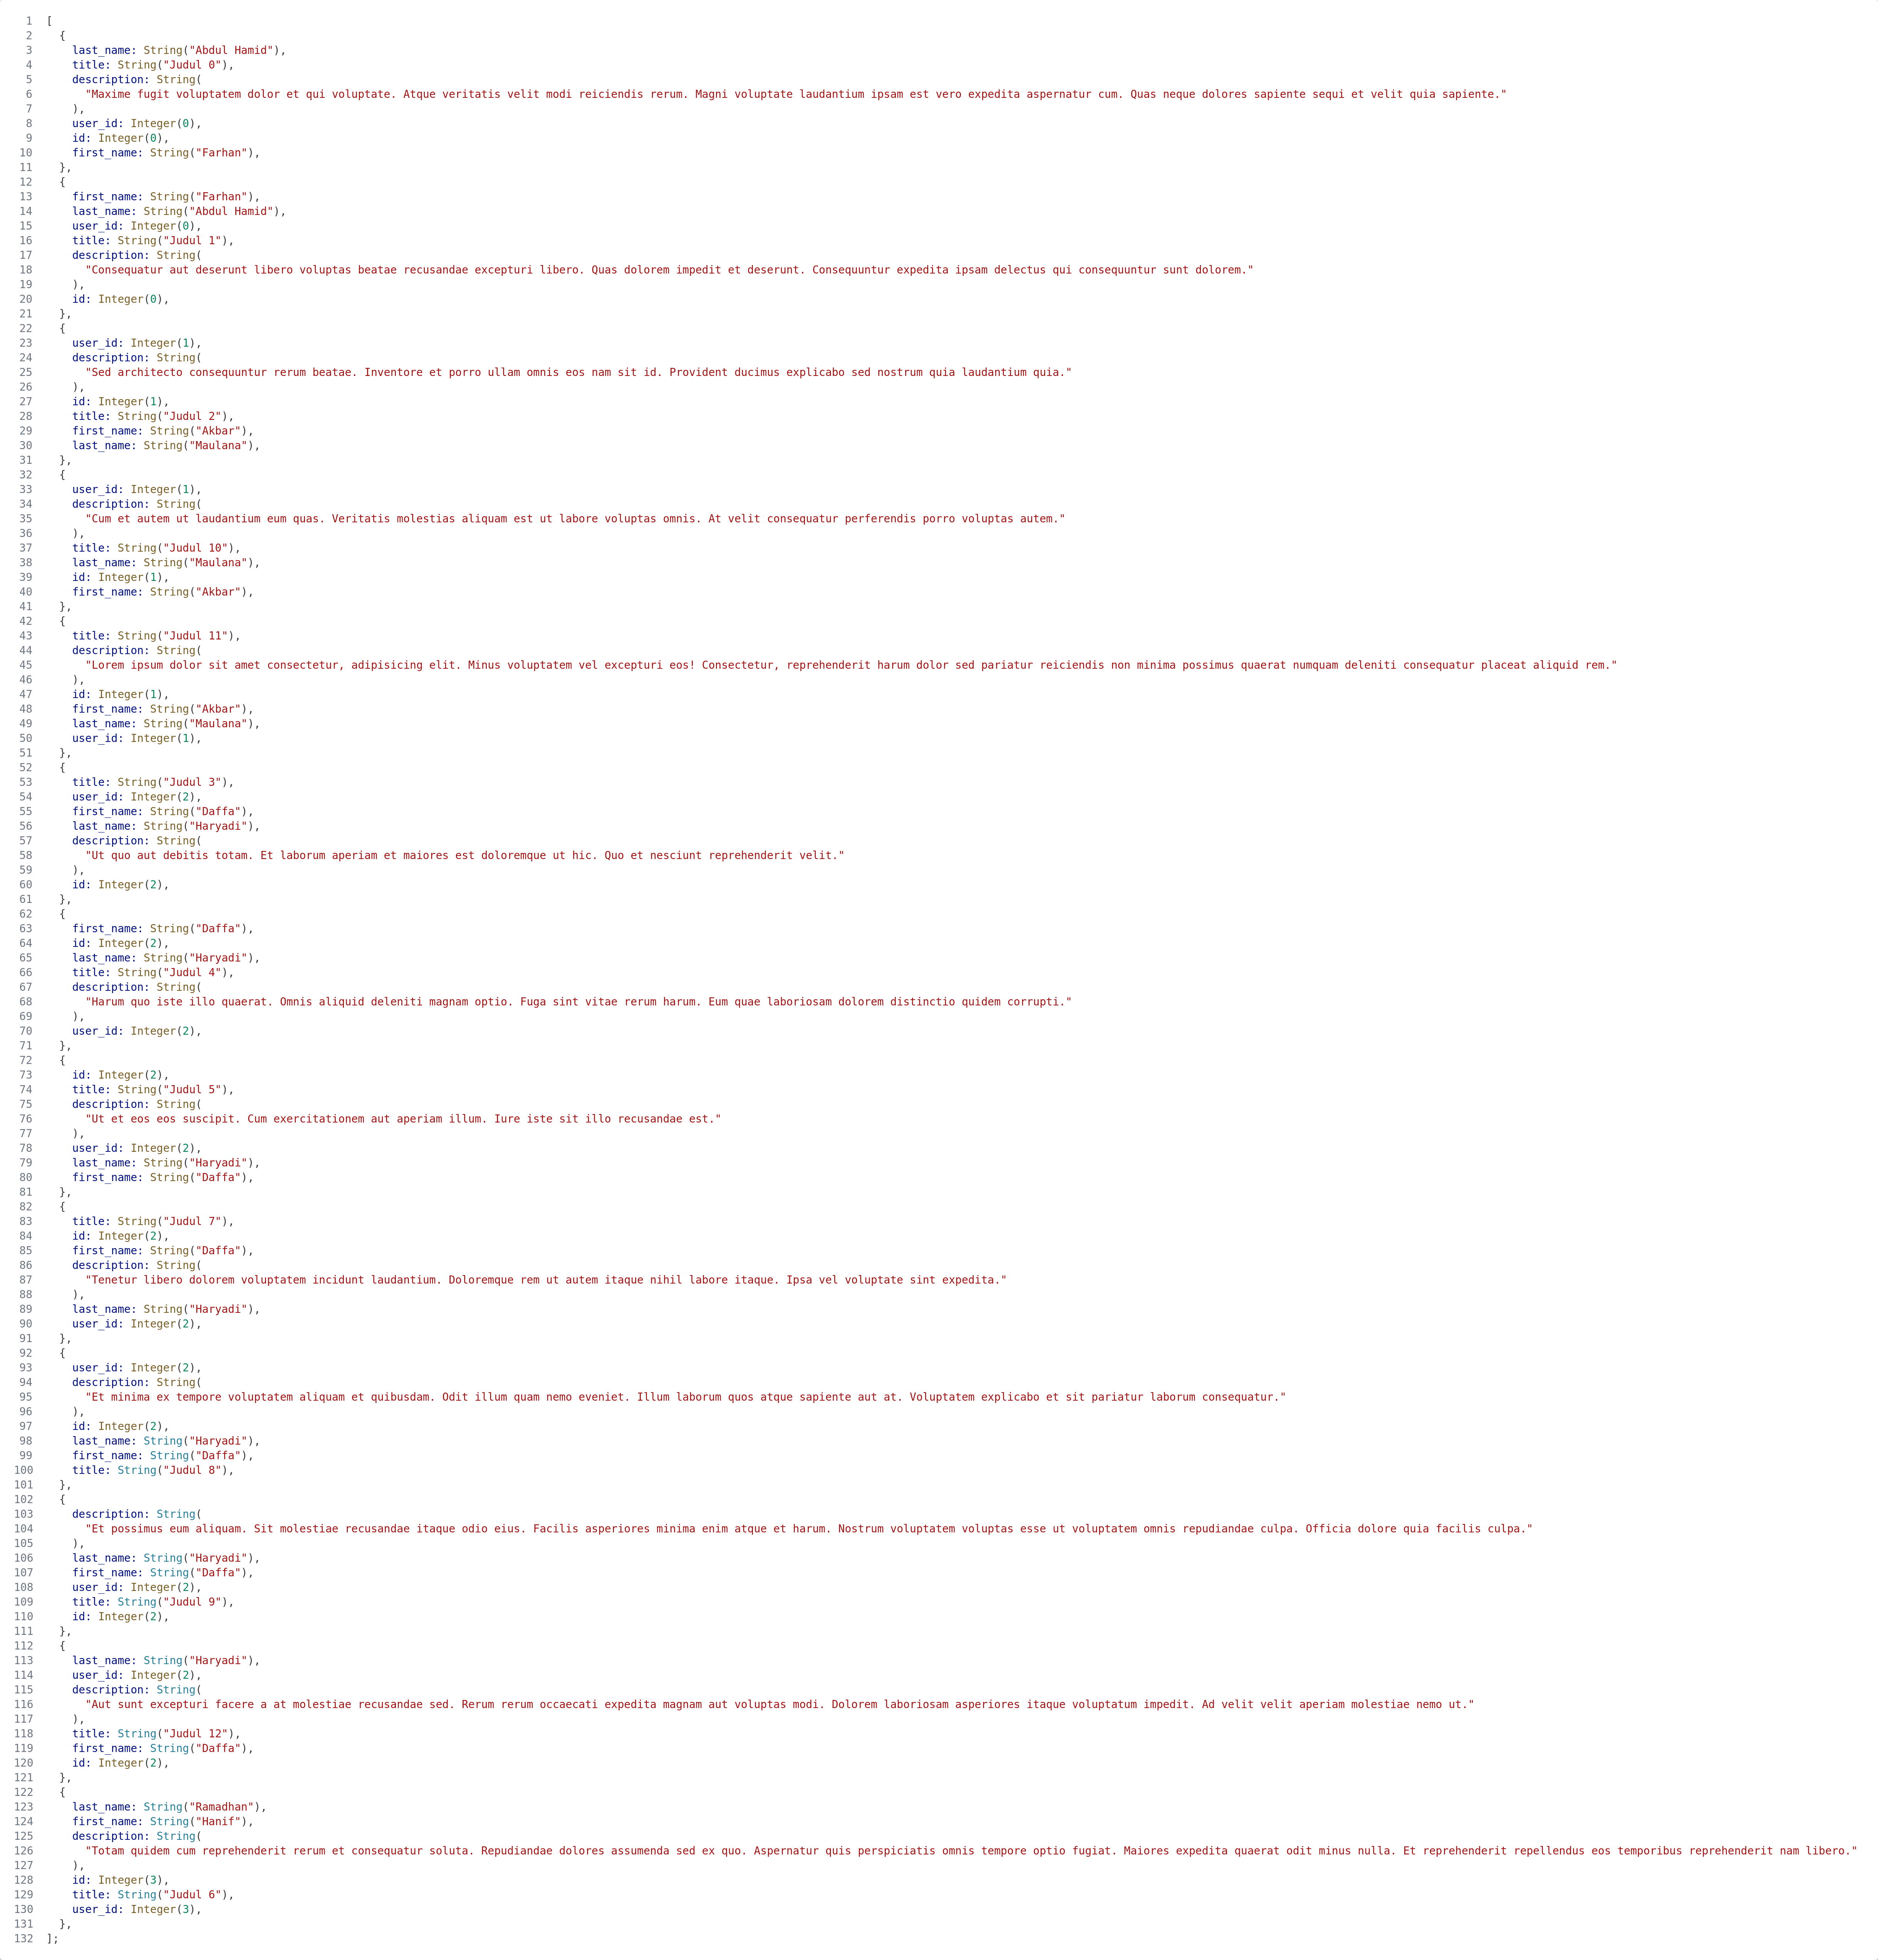
\includegraphics[width=0.9\textwidth]{gambar/bab4/test-join-data-inner-beautify.png}
  	\caption{Hasil data yang telah diformat menggunakan \emph{prettier} (\emph{Extension} VSCode pada Javascript)}
   \end{figure}
  \begin{figure}[H]
  	\centering{}
	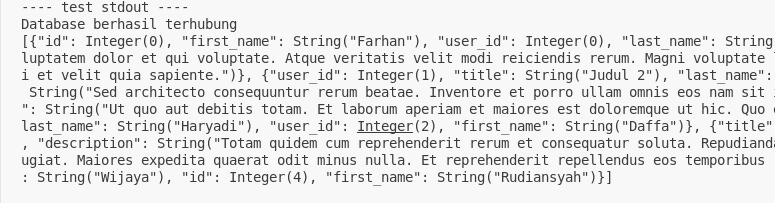
\includegraphics[width=0.6\textwidth]{gambar/bab4/test-join-data-left.png}
  	\caption{Informasi hasil \emph{left join}}
   \end{figure}
    \begin{figure}[H]
  	\centering{}
	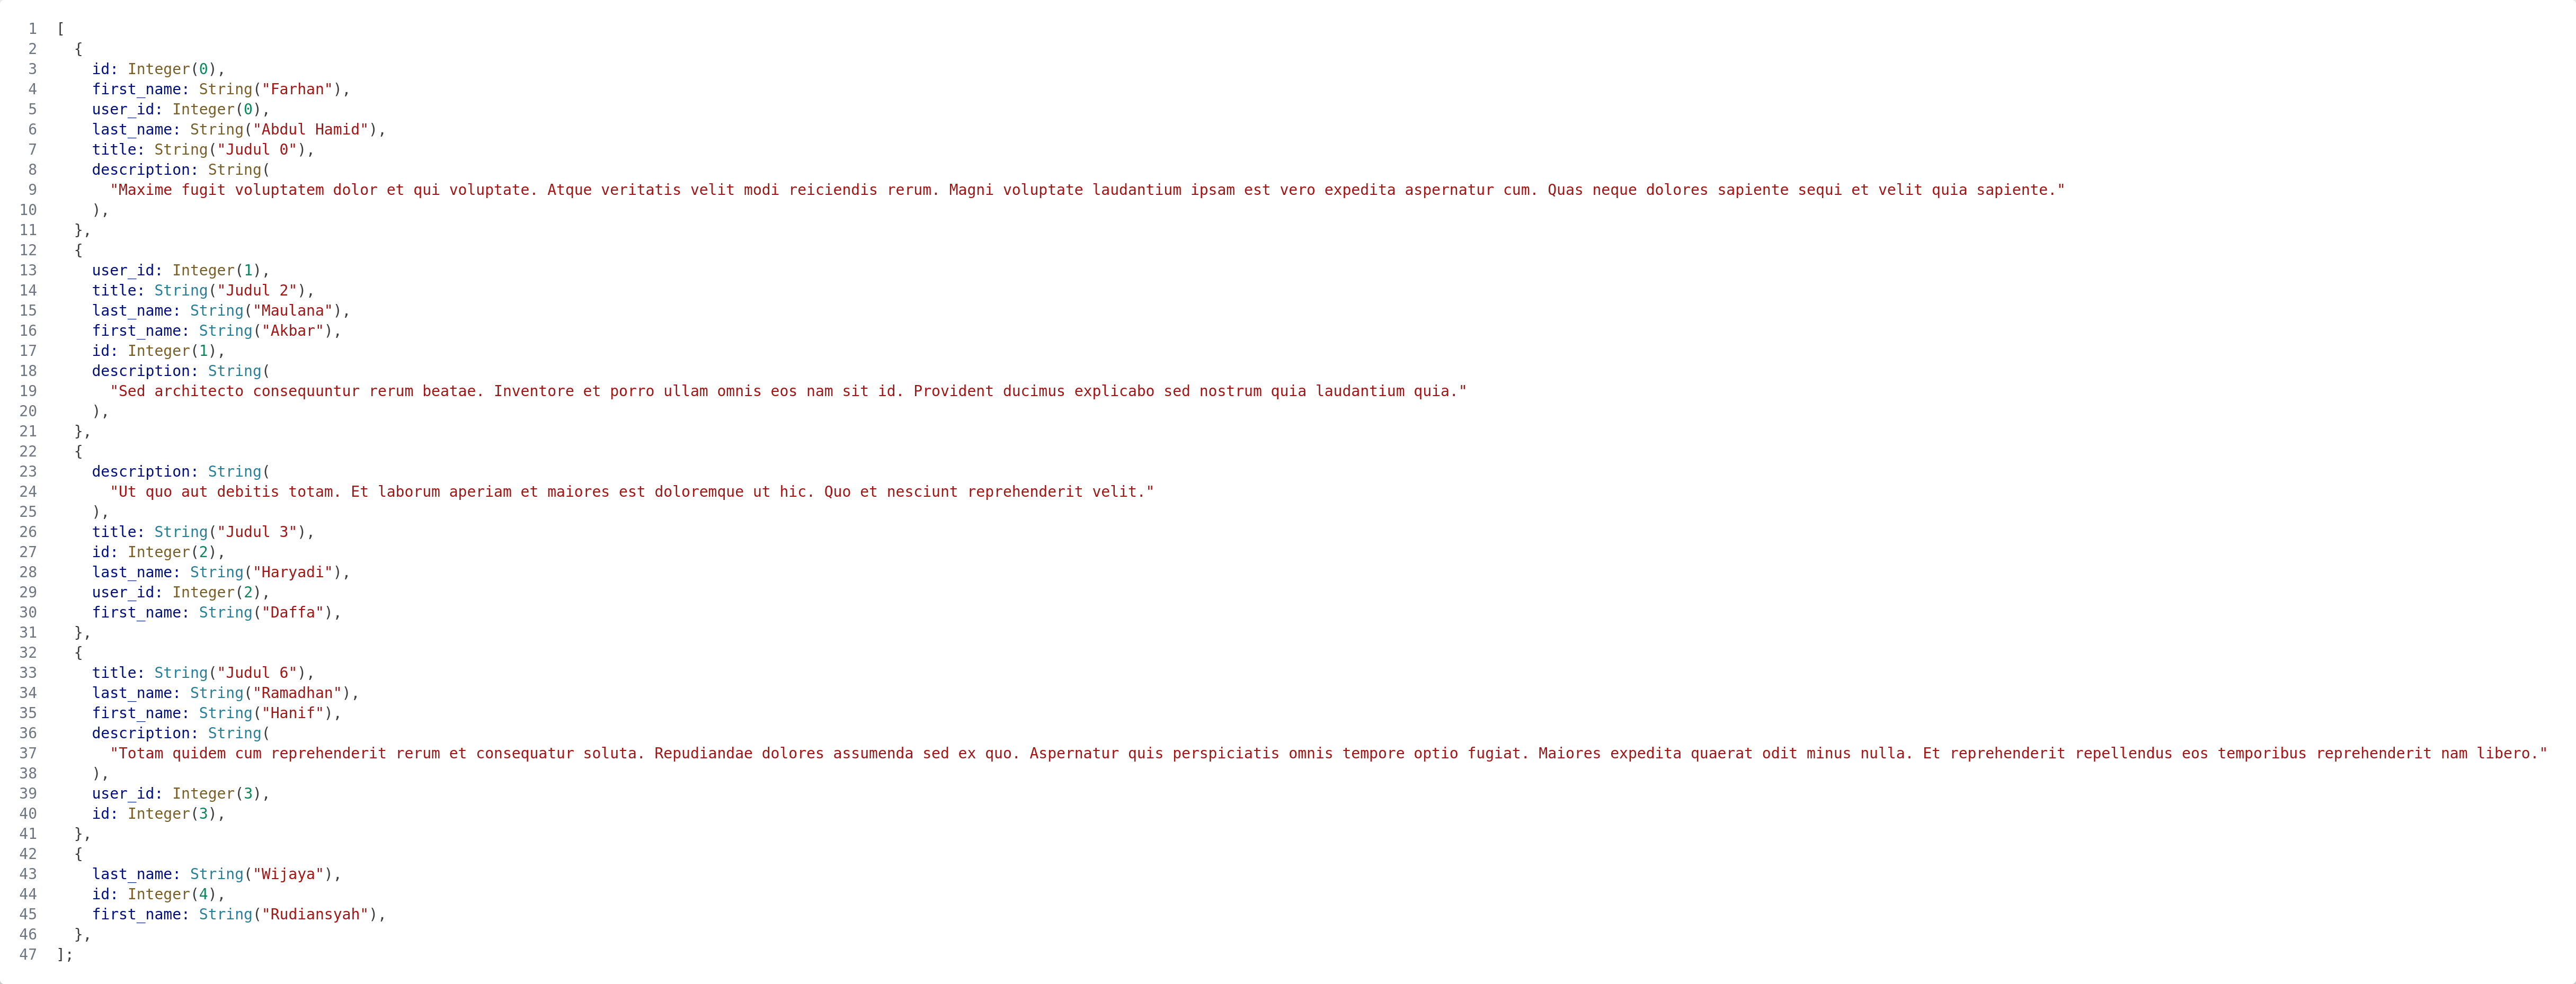
\includegraphics[width=0.9\textwidth]{gambar/bab4/test-join-data-left-beautify.png}
  	\caption{Hasil data yang telah diformat menggunakan \emph{prettier} (\emph{Extension} VSCode pada Javascript)}
   \end{figure}
  \begin{figure}[H]
  	\centering{}
	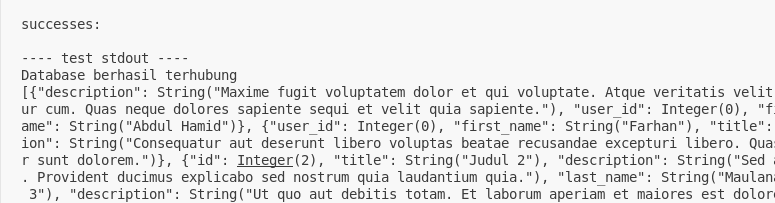
\includegraphics[width=0.6\textwidth]{gambar/bab4/test-join-data-right.png}
  	\caption{Informasi hasil \emph{right join}}
   \end{figure}
    \begin{figure}[H]
  	\centering{}
	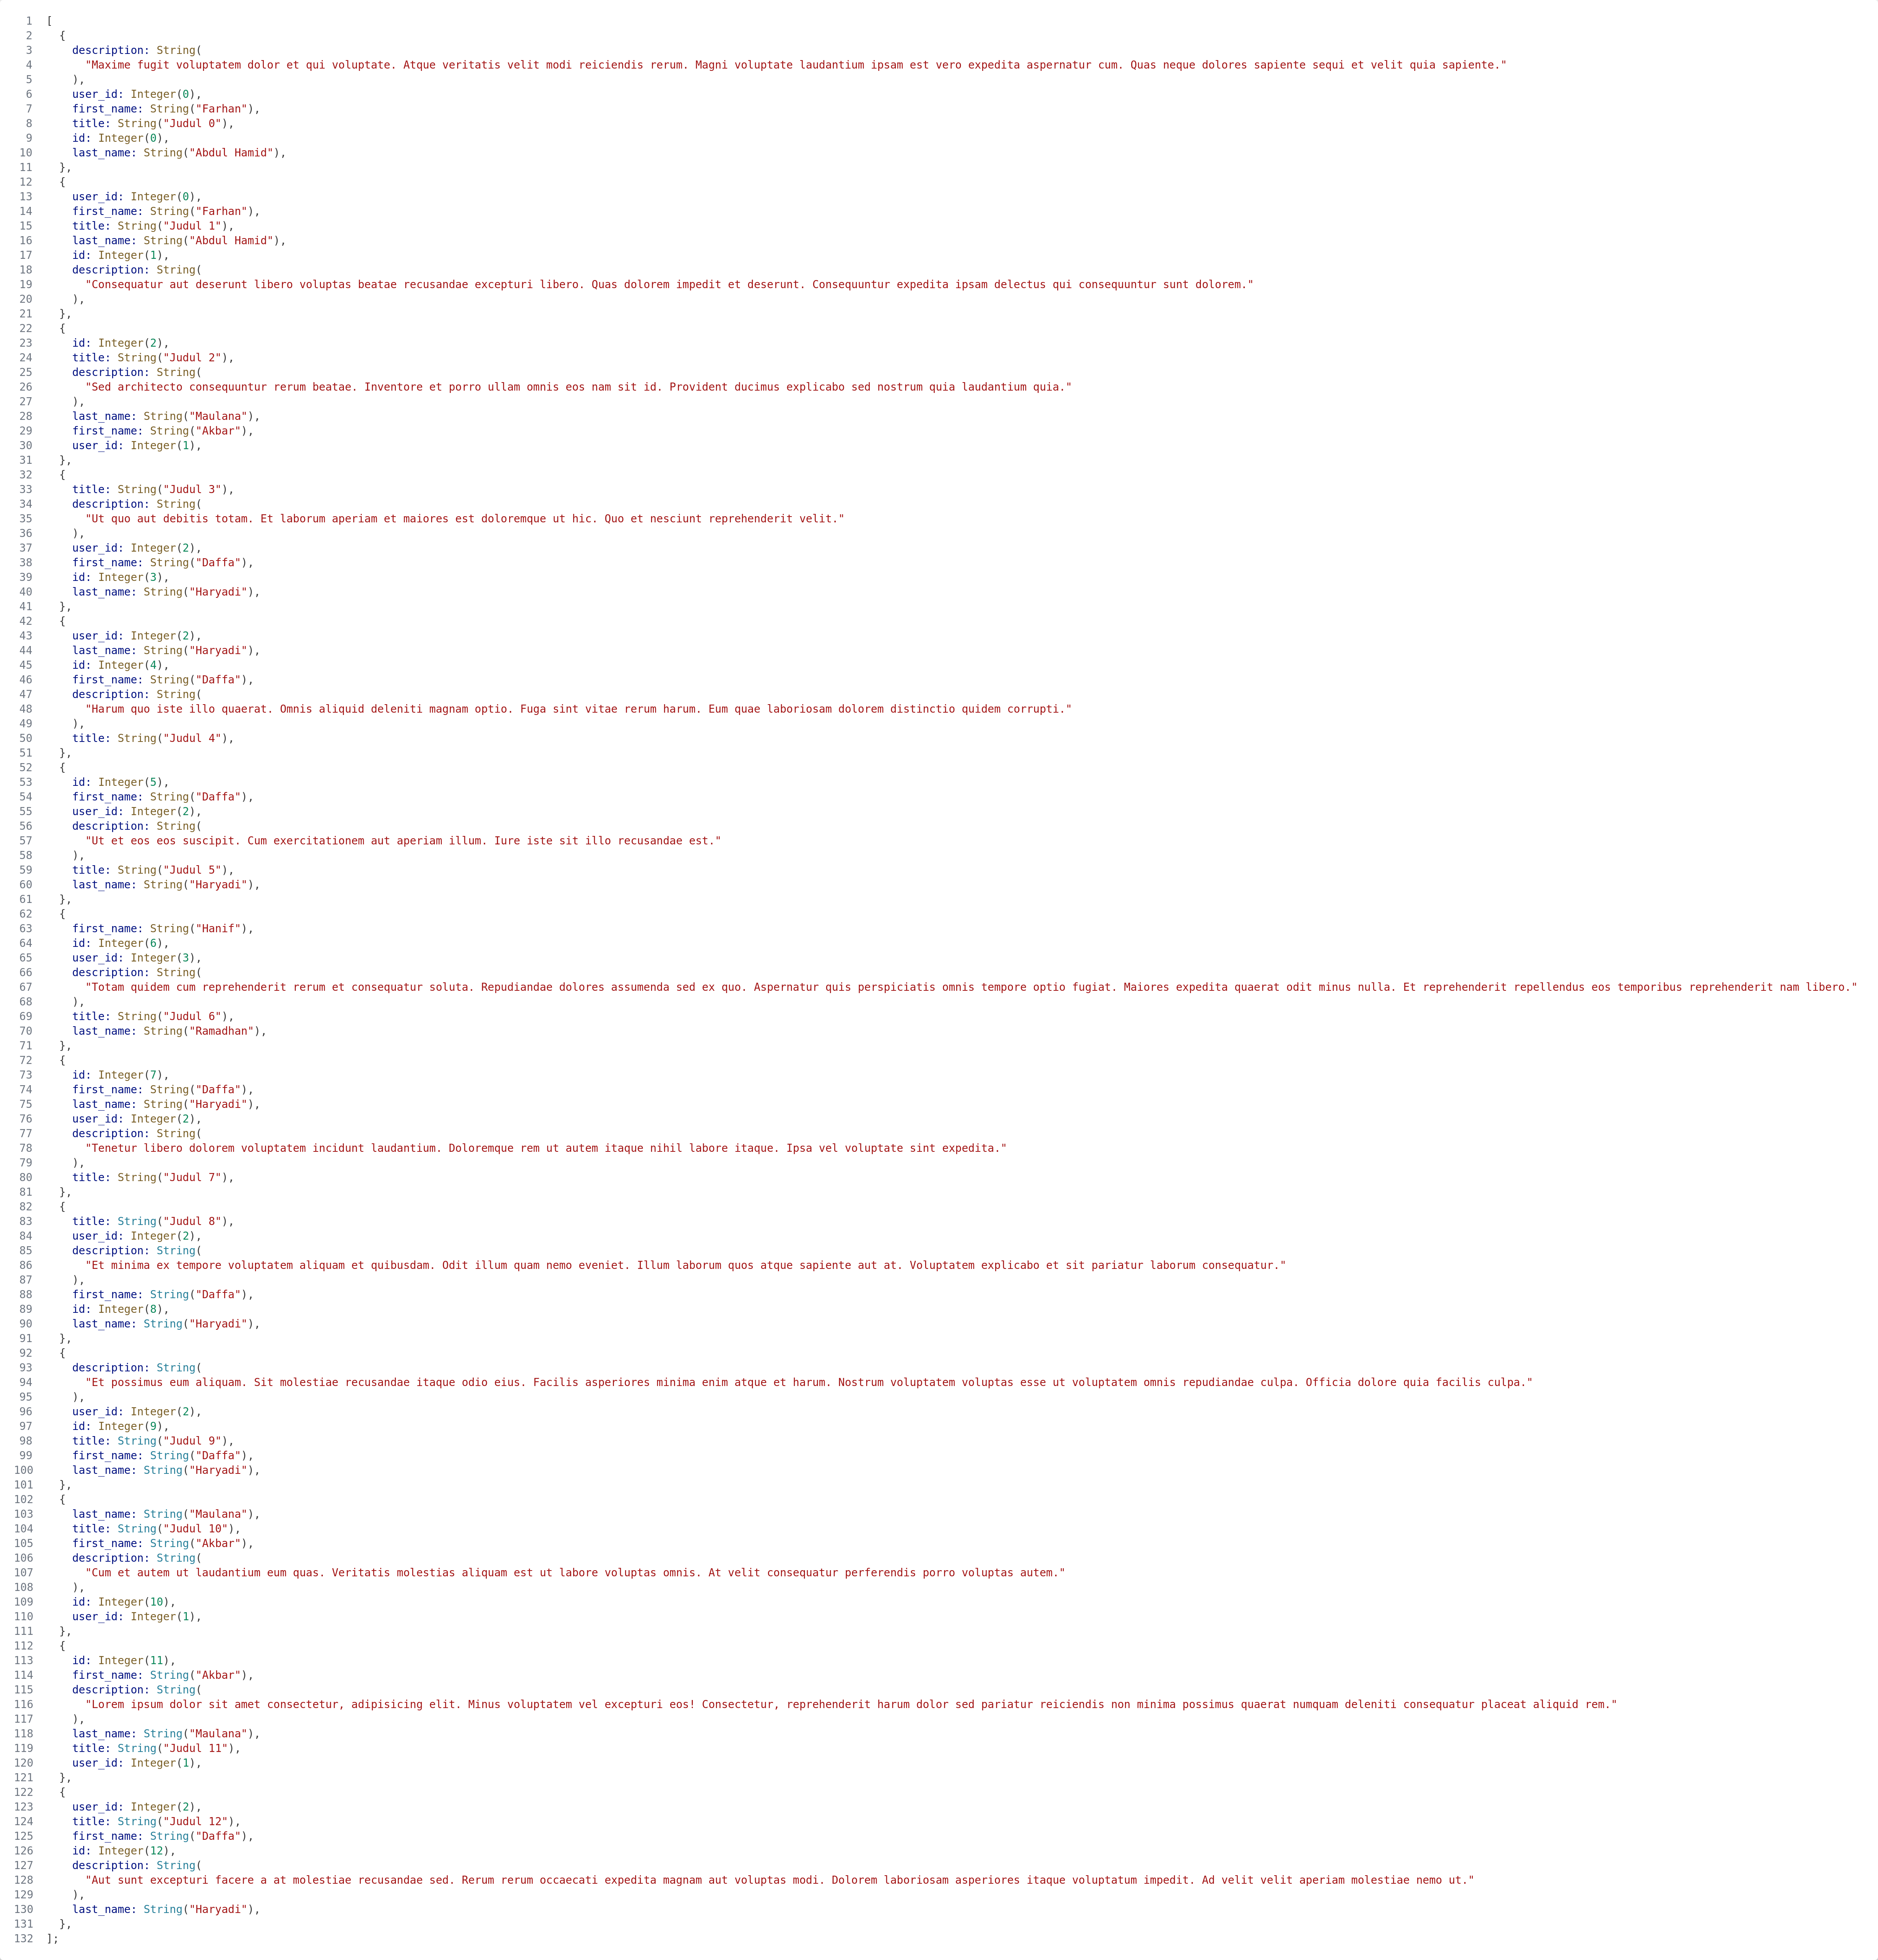
\includegraphics[width=0.9\textwidth]{gambar/bab4/test-join-data-right-beautify.png}
  	\caption{Hasil data yang telah diformat menggunakan \emph{prettier} (\emph{Extension} VSCode pada Javascript)}
   \end{figure}

	\item test\_delete\_data \\
  Pengujian \emph{method} delete data membutuhkan data mana saja yang akan dihapus, tentunya dengan menggunakan kolom tersedia di dalam tabel. Untuk kasus kali ini, data pada tabel users 
  akan dicoba untuk dihapus dengan ketentuan kolom first\_name yang memiliki value "Rudiansyah".
    \begin{figure}[H]
  	\centering{}
	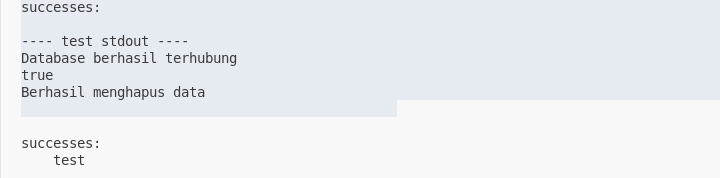
\includegraphics[width=0.6\textwidth]{gambar/bab4/test-delete-data.png}
  	\caption{Informasi hasil penghapusan data}
   \end{figure}
   \begin{figure}[H]
  	\centering{}
	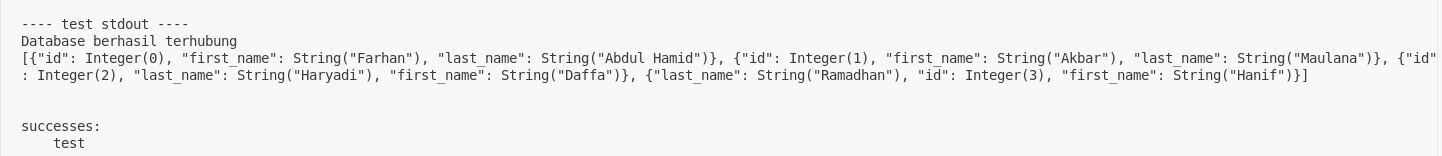
\includegraphics[width=0.6\textwidth]{gambar/bab4/test-hasil-delete.png}
  	\caption{Data tabel \emph{users} setelah value "Rudiansyah" dihapus}
   \end{figure}
  \begin{figure}[H]
  	\centering{}
	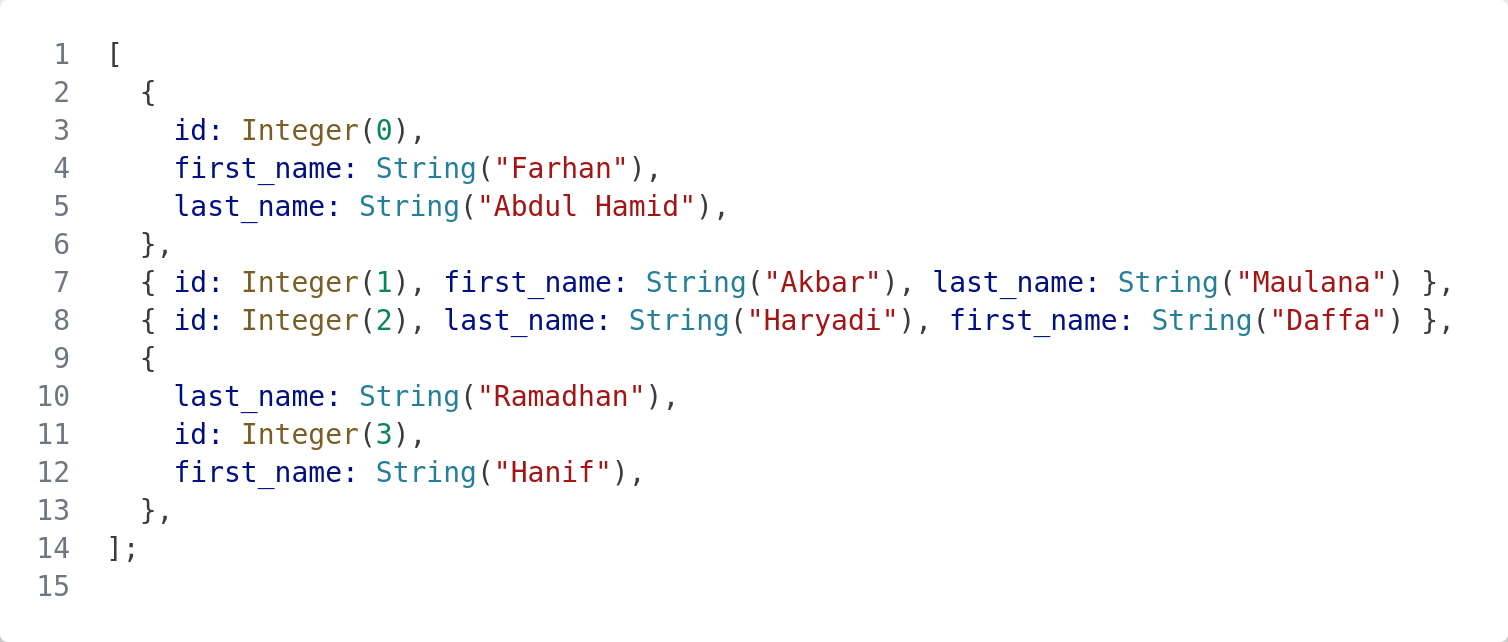
\includegraphics[width=0.9\textwidth]{gambar/bab4/test-hasil-delete-beautify.png}
  	\caption{Data tabel \emph{users} yang telah diformat menggunakan \emph{prettier} (\emph{Extension} \emph{Visual Studio Code} pada Javascript)}
   \end{figure}
\end{enumerate}

\emph{Return} pada setiap \emph{method} didalam \emph{DatabaseInterface} pada pengujian diatas tidak memengaruhi hasil pengujian karena 
untuk menampilkan data, pengujian menggunakan \emph{method} print dari struct yang telah dibuat. Lalu tidak semua \emph{method} yang ada pada \emph{class} \emph{TestDatabaseInterface} digunakan selama pengujian.

\subsection{Pengujian Eksternal}
Untuk melakukan pengujian eksternal diperlukan sebuah \emph{client} untuk memanggil \emph{interface} D-Bus yang telah dibuka. Pada pengujian kali ini, bahasa pemrograman python akan
digunakan beserta dengan library dbus-next. Pengujian akan dilakukan pada proses pembuatan, pengubahan dan penghapusan. Untuk pengambilan data masih belum bisa diuji
sebagaimana yang telah di kutip pada sub bab 4.1.11. Berikut adalah isian dari program \emph{client} menggunakan bahasa pemrograman python.

 \begin{figure}[H]
  	\centering{}
	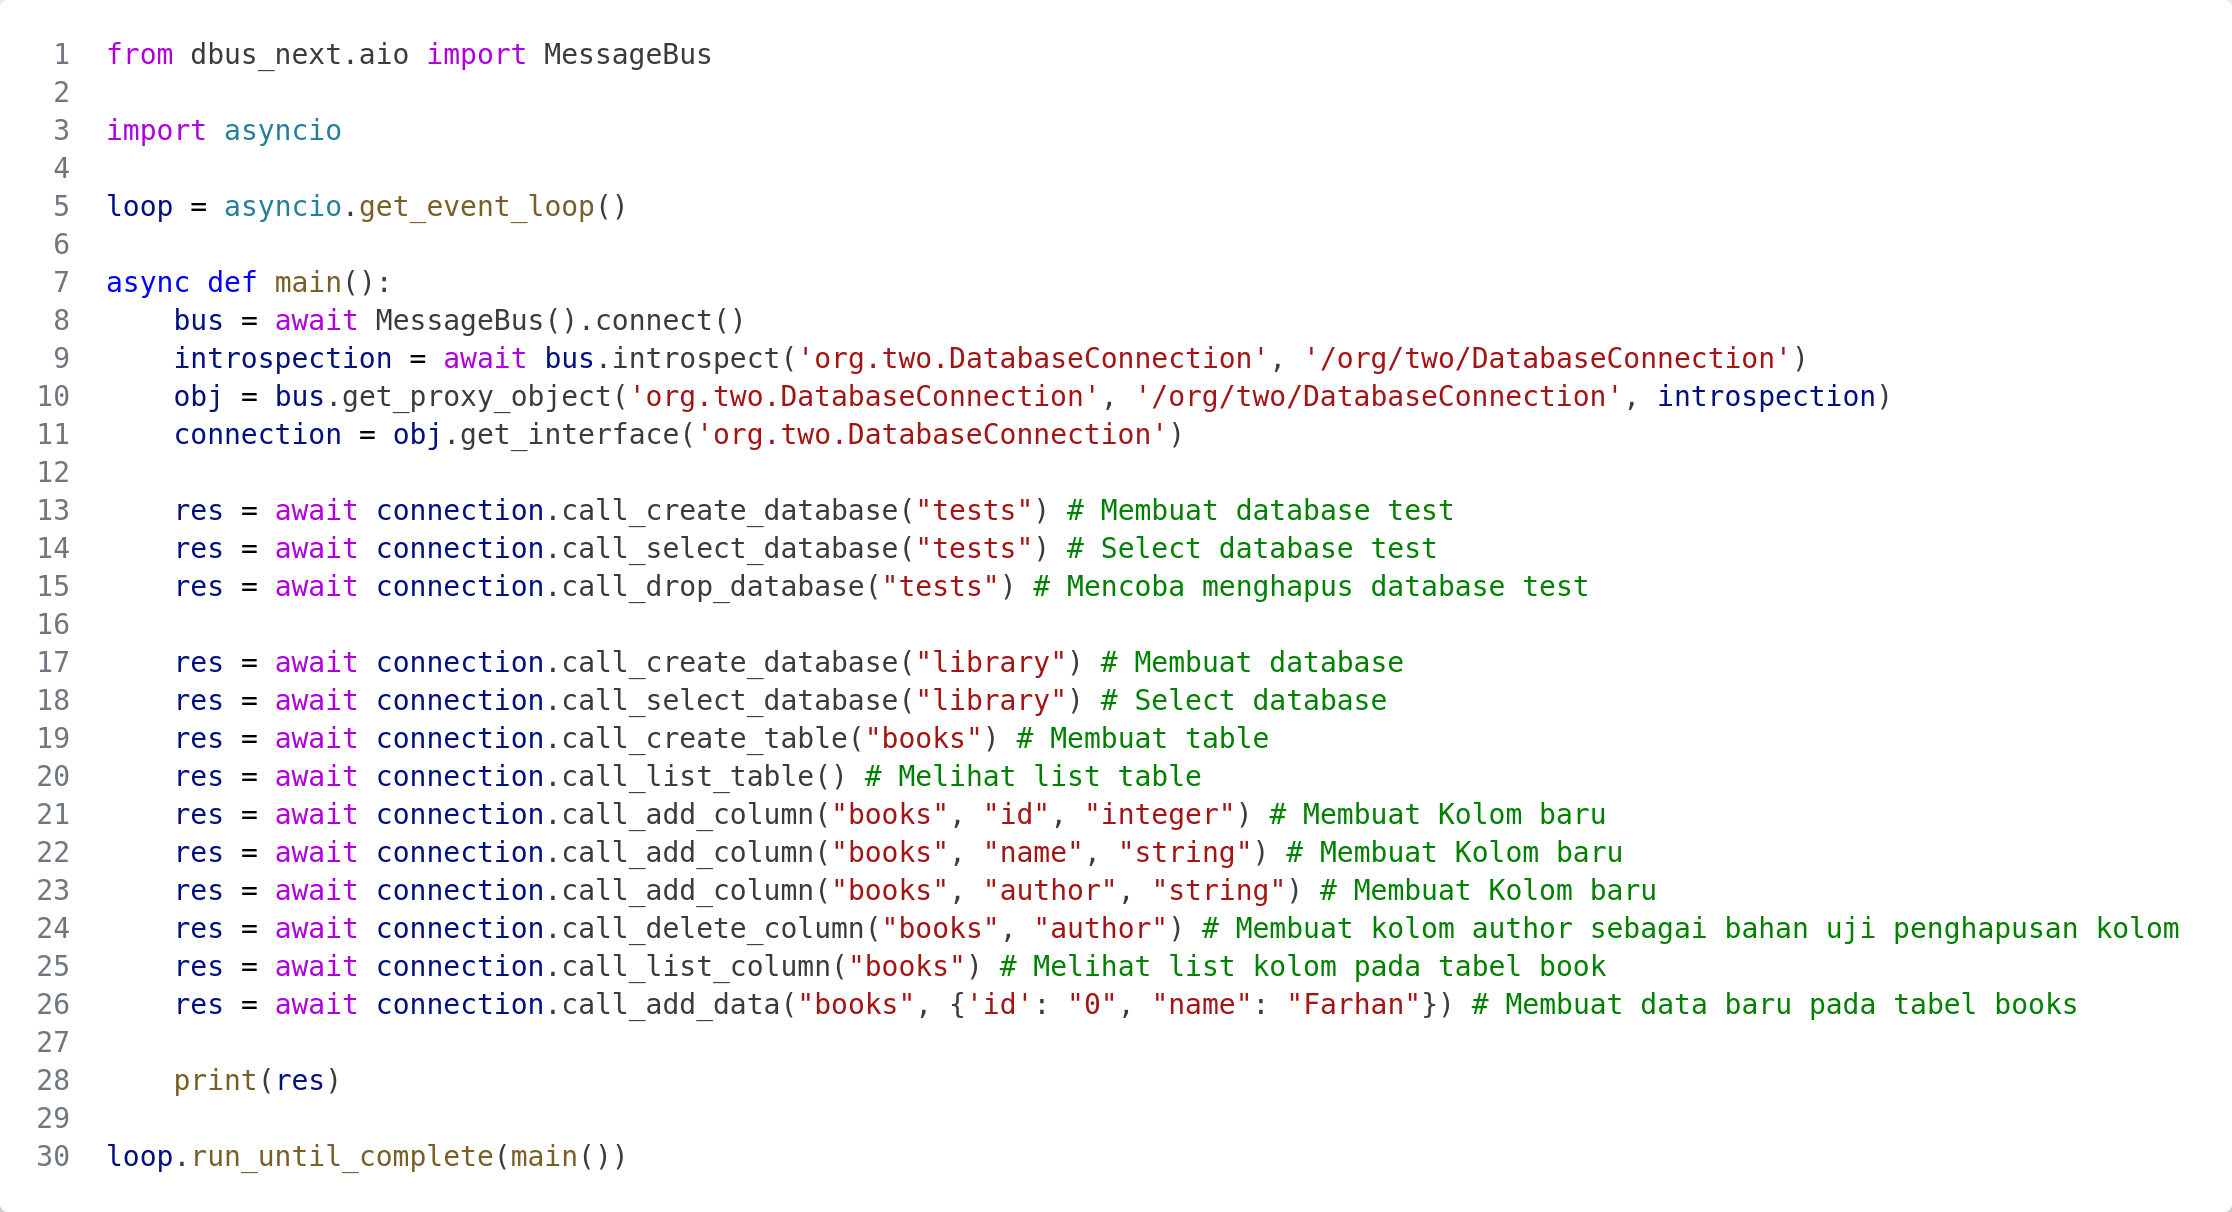
\includegraphics[width=0.8\textwidth]{gambar/bab4/uji-client.png}
  	\caption{Isi program pengujian \emph{client} dengan bahasa pemrograman Python}
   \end{figure}

    \begin{figure}[H]
  	\centering{}
	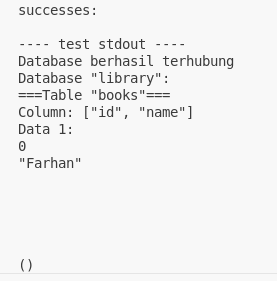
\includegraphics[width=0.6\textwidth]{gambar/bab4/hasil-uji-client.png}
  	\caption{Informasi hasil pengujian client}
   \end{figure}

Hasil dari pengujian \emph{client} dijalankan dengan \emph{method} print pada \emph{class} TestDatabaseInterface. \emph{Method} tersebut merupakan \emph{method} yang berguna untuk melihat keseluruhan
data yang tersimpan pada suatu \emph{database}.

\subsection{Pengujian Internal dengan Data Hasil \emph{Crawling}}
\emph{Database Engine} yang dikembangkan pada saat ini ditujukan untuk pengembangan sistem \emph{crawling} pada penelitian terakhir (\cite{ridho2024}). Karena alasan tersebut, pengujian menggunakan
data hasil \emph{crawling} pada penelitian sebelumnya (\cite{ridho2024}) akan dilakukan. Untuk pengujian tidak semua tabel akan digunakan, hanya 2 tabel hasil \emph{crawling} saja yaitu tabel bernama page\_information dan crawling.
Dalam tabel tersebut terdapat berbagai macam data, namun dikarenakan pada database saat ini hanya mendukung 2 tipe data yaitu \emph{string} dan \emph{integer}, maka untuk tipe data lain diluar dari 2 tipe data tersebut,
akan dirubah menjadi \emph{string}. Sebanyak 10 baris dari tabel page\_information akan digunakan, data tersebut dapat dilihat pada \emph{file} crawl\_information.json dalam \emph{folder} test-data.
Proses pengujian dilakukan dengan tahapan berikut:

\begin{enumerate}
	\item Membuat \emph{database}
	\item Membuat \emph{table} crawling dengan \emph{table} page\_information
	\item Melengkapi kolom pada \emph{table} crawling
	\item Mengisi data pada \emph{table} crawling
	\item Melengkapi kolom pada \emph{table} page\_information
	\item Mengisi data pada \emph{table} page\_information
	\item Menampilkan data yang telah terisi
\end{enumerate}

Dari hasil pengujian tersebut didapatkan bahwa, penyimpanan dan pengambilan dapat berjalan dengan baik. Namun hal tersebut hanya berlaku untuk huruf latin, untuk huruf-huruf bahasa lain seperti
bahasa china, jepang, arab dan lainnya masih belum dapat tersimpan dengan benar. Permasalahan ini harus ditelusuri lebih lanjut, namun ada kemungkinan bahwa penyimpanan 1 huruf selain huruf latin memiliki
ukuran yang berbeda dengan huruf latin. Berikut adalah contoh kesalahan penyimpanan dan penampilan data pada bahasa non latin:

\begin{figure}[H]
	\centering{}
	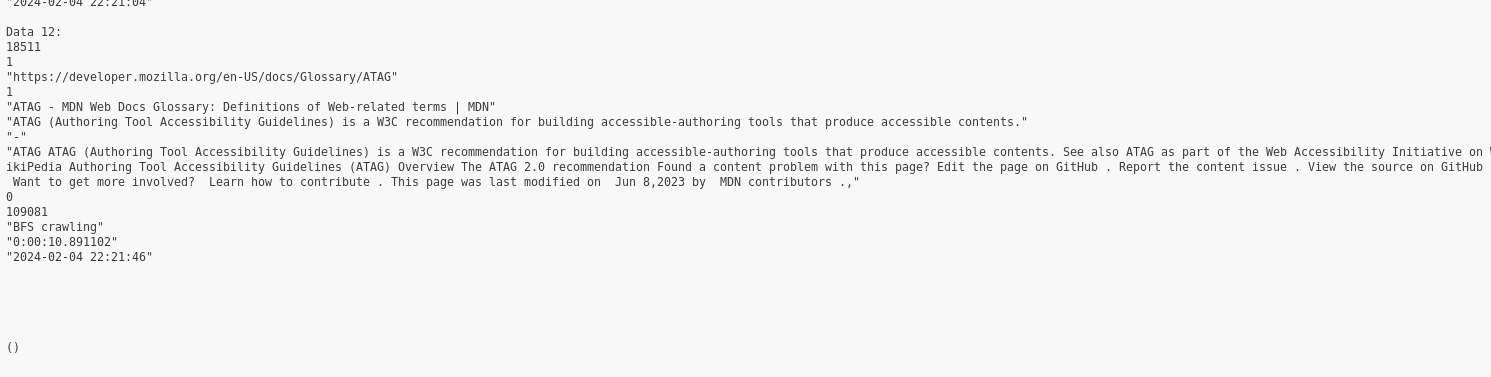
\includegraphics[width=0.95\textwidth]{gambar/bab4/hasil-pengujian-data-hasil-crawling.png}
	\caption{Informasi hasil pengujian data \emph{crawling}}
\end{figure}


\subsection{Hasil Implementasi}

Dari implementasi dan pengujian yang dilakukan pada sub bab sebelumnya, maka didapatkan sebuah \emph{database engine} baru yang dikembangkan dengan bahasa pemrograman Rust.
Pemrosesan yang terjadi dalam \emph{database engine} yang telah dibuat dapat dilihat pada setiap method-method yang telah dibuat. Pemrosesan tersebut mulai dari mengambil data,
menyimpan data, mengubah data dan menghapus data. Dari hasil pengujian pun dapat terlihat bahwa \emph{database} telah berhasil disimpan secara persisten dalam sebuah sebuah \emph{file}.
Tidak hanya itu, pola dan metode penyimpanan pun dapat terlihat dari urutan \emph{byte} yang disimpan pada \emph{file}. Dengan begitu pengembang ke depannya dapat mengubah dan menyesuaikan pola
pemrosesan data di dalam \emph{database} baru ini jika menemukan pola atau algoritma yang lebih efisien. Terlebih jika di kedepan hari \emph{database engine} ini akan di implementasikan pada 
\emph{distributed database}, maka algoritma sinkronisasi dapat di terapkan langsung di dalam \emph{class} Schema yang telah dibuat. Algoritma yang dipilih dikembalikan kepada pengembang \emph{database
engine} ini di kemudian hari.

Meski demikian masih terdapat banyak fitur dari \emph{database} ini yang belum berjalan dengan baik dan memerlukan penyempurnaan. Berikut adalah hal-hal yang dapat disempurnakan pada fitur \emph{database
engine} ini, yaitu:
\begin{enumerate}
	\item Melengkapi metode-metode eksternal untuk \emph{client} \\
  	Belum semua \emph{method} yang ada pada \emph{DatabaseInterface} terimplementasi pada \emph{DatabaseConnection}, sehingga membuat \emph{client} belum bisa menggunakan \emph{database engine} sepenuhnya.
	
	\item Memperbaiki return \emph{indexing} pada \emph{join} \\
	Dengan menerapkan \emph{indexing} yang ada pada \emph{database engine} saat ini, maka fitur \emph{join} tabel masih belum bisa berjalan dikarenakan tidak dapat mengembalikan data ke \emph{DatabaseConnection}.

	\item Menambahkan utilitas pada fitur \emph{join} \\
	Membuat fitur \emph{joining} untuk 3 tabel atau lebih, serta membuat constraint pada column yang menjadi key antar tabel.
	
	\item Melihat metadata pada column di \emph{database} \\
	Saat ini fitur untuk melihat list column, baru mengembalikan nama kolom saja dari tabel.

	\item Menambahkan metadata pada \emph{database} dan table \\
	Metadata yang umumnya ada pada fitur \emph{database management} seperti created\_at, increment, uniqueId dan lainnya.

	\item Menambahkan tipe data lain \\
	Menambahkan tipe data lain karena saat ini hanya bisa mendukung 2 tipe data yaitu String dan Integer.

	\item Pengubahan default value \\
	Menambahkan perubahan nilai default pada cell yang ada di \emph{database} agar nilai default dari sebuah cell dapat diubah.

	\item Membuat multi connection \\
	Saat ini koneksi yang dapat ditangani hanya 1 koneksi, jika digunakan untuk 2 koneksi \emph{client}, maka dikhawatirkan terdapat data yang tidak sinkron.

	\item Membuat kompatibilitas terhadap bahasa non latin \\
	Pada sistem \emph{database engine} yang berjalan saat ini, masih belum dapat menyimpan dan menampilkan data dengan bahasa non latin. Kemungkinan hal ini terjadi
	dikarenakan bahasa non latin memiliki jumlah \emph{byte} yang berbeda untuk satu karakter dibanding dengan satu karakter huruf latin.

	\item Pembuatan \emph{folder} \emph{schema} dan \emph{index} secara otomatis  \\
	Setelah melakukan proses \emph{build}, jika hasil \emph{build database engine} ingin dikirim ke perangkat lain, maka untuk saat ini \emph{folder} \emph{schema} dan \emph{folder}
	\emph{index} harus dibuat manual. 

	\item Memperbaiki dan menyempurnakan penanganan \emph{error} \\
  	Error yang ada pada saat ini hanya bisa dilihat dari server dan belum di handle dengan baik pada \emph{client}. Hal ini dapat menyebabkan \emph{client} tidak tau pasti penyebab error.
	Terdapat beberapa \emph{error} lain seperti saat hendak melakukan pembuatan database tanpa adanya \emph{folder} \emph{schema} dan \emph{index}. Jika tidak ada kedua \emph{folder} tersebut 
	maka database tidak terbuat, dan langsung memunculkan pesan "\emph{Database Created!}". Tentunya pesan yang disampaikan
	tidaklah sesuai, hal ini dikarenakan penanganan \emph{error} di \emph{Database Interface} masih belum baik. Tidak menutupi kemungkinan bahwa masih terdapat
	penanganan error lain yang harus ditingkatkan seperti jika path dari D-Bus sudah dipakai oleh sistem lain dan lainnya.

\end{enumerate}

\section{Sumber dan Orisinalitas \emph{code}}
Dalam pengembangan \emph{database engine}, berbagai macam sumber \emph{code} pihak lain digunakan sebagai referensi. Sumber-sumber tersebut dari beberapa \emph{website} 
serta dokumentasi langsung bahasa pemrograman dan \emph{library} yang digunakan selama pengembangan. Salah satu bagian penting pada pengembangan yang didapatkan dari 
referensi lain adalah proses perubahan dari sebuah data menjadi bentuk byte serta mengembalikannya dalam bahasa pemrograman rust. Hasil akhir dari \emph{source code} dapat dilihat pada \emph{link} berikut.

\begin{center}
	\href{https://github.com/arhandev11/database-engine}{https://github.com/arhandev11/database-engine}
\end{center}

Selain itu, sumber untuk melakukan penerapan metode \emph{waterfall} juga digunakan sebagai pembanding dengan penulisan yang dibuat. Hal ini dilakukan karena selama 
pengembangan berlangsung masih belum menggunakan metode \emph{waterfall}. Sumber lain seperti dokumentasi resmi postgresql dan lainnya digunakan sebagai
sumber pengetahuan dan pertimbangan dalam pengembangan \emph{database engine}. Penggunaan \emph{Artificial Intelligence} dengan model \emph{Gemini 2.5 pro} dan \emph{Chatgpt (Versi o4-mini-high, 4.1 dan 5)} juga
digunakan dalam memahami isi \emph{paper} serta dalam membantu membuat penulisan dan \emph{formatting} menggunakan \emph{latex}.

% Baris ini digunakan untuk membantu dalam melakukan sitasi
% Karena diapit dengan comment, maka baris ini akan diabaikan
% oleh compiler LaTeX.
\begin{comment}
\bibliography{daftar-pustaka}
\end{comment}

%!TEX root = ../main.tex
%-------------------------------------------------------------------------------
%                          BAB V
%               		KESIMPULAN DAN SARAN
%-------------------------------------------------------------------------------

\chapter{KESIMPULAN DAN SARAN}

\section{Kesimpulan}

Berdasarkan hasil implementasi dan pengujian yang sudah dijalankan maka terdapat beberapa kesimpulan sebagai berikut:

\begin{enumerate}
	\item Untuk membuat \emph{database engine} yang menjaga integritas data, maka harus memikirkan bagaimana cara
	database tersebut disimpan pada \emph{filesystem}. Jenis data yang disimpan juga harus dipikirkan untuk memastikan
	data yang telah berubah menjadi \emph{byte} dapat kembali menjadi nilai asli dan tipe aslinya walaupun pada fitur saat ini 
	masih memiliki keterbatasan dalam pengembalian datanya.
	\item Penyimpanan data pada \emph{filesystem} harus konsisten agar tidak terdapat data yang hilang. Karena berbeda 1 urutan saja
	dapat menghancurkan data-data yang tersimpan diurutan lainnya.
	\item Fitur-fitur untuk mengolah data yang disimpan pada \emph{filesystem} dapat dikelola oleh atribut dan \emph{method}
	pada bahasa pemrograman yang digunakan. Sehingga harus mempertimbangkan \emph{method} yang mana saja yang dapat di akses oleh \emph{client}.
	\item Tipe data yang terdapat pada \emph{database} harus kompatibel untuk berbagai bahasa untuk memastikan antara server dan\emph{client}dapat saling
	tukar menukar data.
	\item Implementasi algoritma sinkronisasi sangat memungkinkan untuk diterapkan di dalam sistem \emph{database} karena alur awal penerimaan data sampai
	penyimpanan data dapat dilihat secara langsung. Tak hanya algoritma, metode penyimpanan pada \emph{filesystem} dan \emph{index} juga bisa lebih dikembangkan lagi
	untuk mencari performa yang paling optimal.
	\item Penanganan penyimpanan data untuk bahasa non latin memiliki tahapan yang berbeda dikarenakan cara yang diterapkan pada saat ini
	masih belum berhasil.
\end{enumerate}

\section{Saran}

Berdasarkan hasil implementasi dan pengujian yang sudah dijalankan, terdapat beberapa saran untuk menyempurnakan \emph{database engine} di kemudian hari, yaitu:

\begin{enumerate}
	\item Mencoba memperbaiki kekurangan pada \emph{database engine} sesuai dengan yang dibahas pada sub bab 4.2.4. Tujuannya adalah agar \emph{database engine} yang telah dibuat 
	saat ini dapat diimplementasikan pada sistem lain yang sudah berjalan.
	\item Mengimplementasikan fitur distribusi \emph{database}, agar dapat segera digunakan pada sistem \emph{crawling} untuk \emph{search engine}. Salah satu langkah utamanya
	adalah dengan mencari algoritma sinkronisasi yang paling optimal dan efisien yang dapat diterapkan pada \emph{database engine} saat ini.
	\item Implementasikan lebih dalam fitur-fitur koneksi yang ada pada D-Bus agar komunikasi ke \emph{client} dapat berjalan lebih baik.
	\item Sebelum melanjutkan pengembangan \emph{database}, sangat disarankan untuk mempelajari konsep dan paradigma yang ada di bahasa pemrograman rust agar dapat mengimplementasikan
	fitur-fitur lain menjadi lebih baik ke depannya.
\end{enumerate}


% Baris ini digunakan untuk membantu dalam melakukan sitasi
% Karena diapit dengan comment, maka baris ini akan diabaikan
% oleh compiler LaTeX.
\begin{comment}
\bibliography{daftar-pustaka}
\end{comment}


%-----------------------------------------------------------------
%Disini akhir masukan Bab
%-----------------------------------------------------------------


%-----------------------------------------------------------------
% Disini awal masukan untuk Daftar Pustaka
% - Daftar pustaka diambil dari file .bib yang ada pada folder ini
%   juga.
% - Untuk memudahkan dalam memanajemen dan menggenerate file .bib
%   gunakan reference manager seperti Mendeley, Zotero, EndNote,
%   dll.
%-----------------------------------------------------------------
% \bibliography{daftar-pustaka}
% \bibliographystyle{apalike}
\addcontentsline{toc}{chapter}{DAFTAR PUSTAKA}
\singlespacing{}
\printbibliography{}
\nocite{*}

%-----------------------------------------------------------------
%Disini akhir masukan Daftar Pustaka
%-----------------------------------------------------------------


%!TEX root = ../main.tex
\addcontentsline{toc}{chapter}{LAMPIRAN}
\appendix

\chapter{Dokumentasi Source Code}

\begin{figure}[H]
  \centering{}
	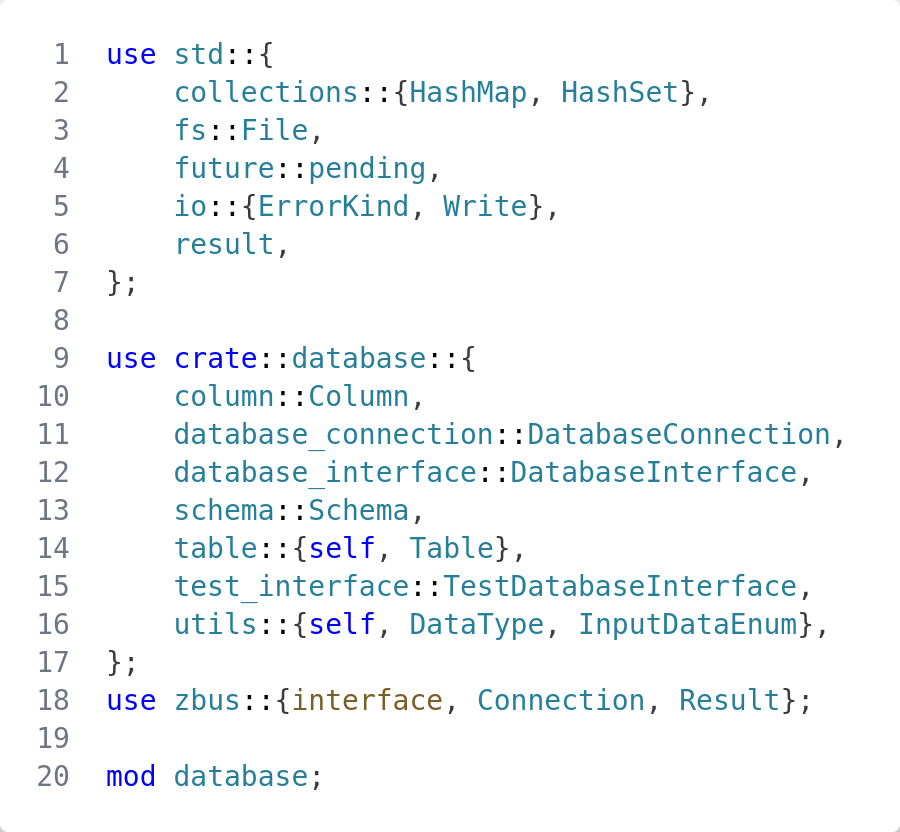
\includegraphics[width=0.9\textwidth]{gambar/lampiran/file-import-main.png}
  \caption{\emph{Import} dalam \emph{file} main.rs}
\end{figure}

\begin{figure}[H]
  \centering{}
	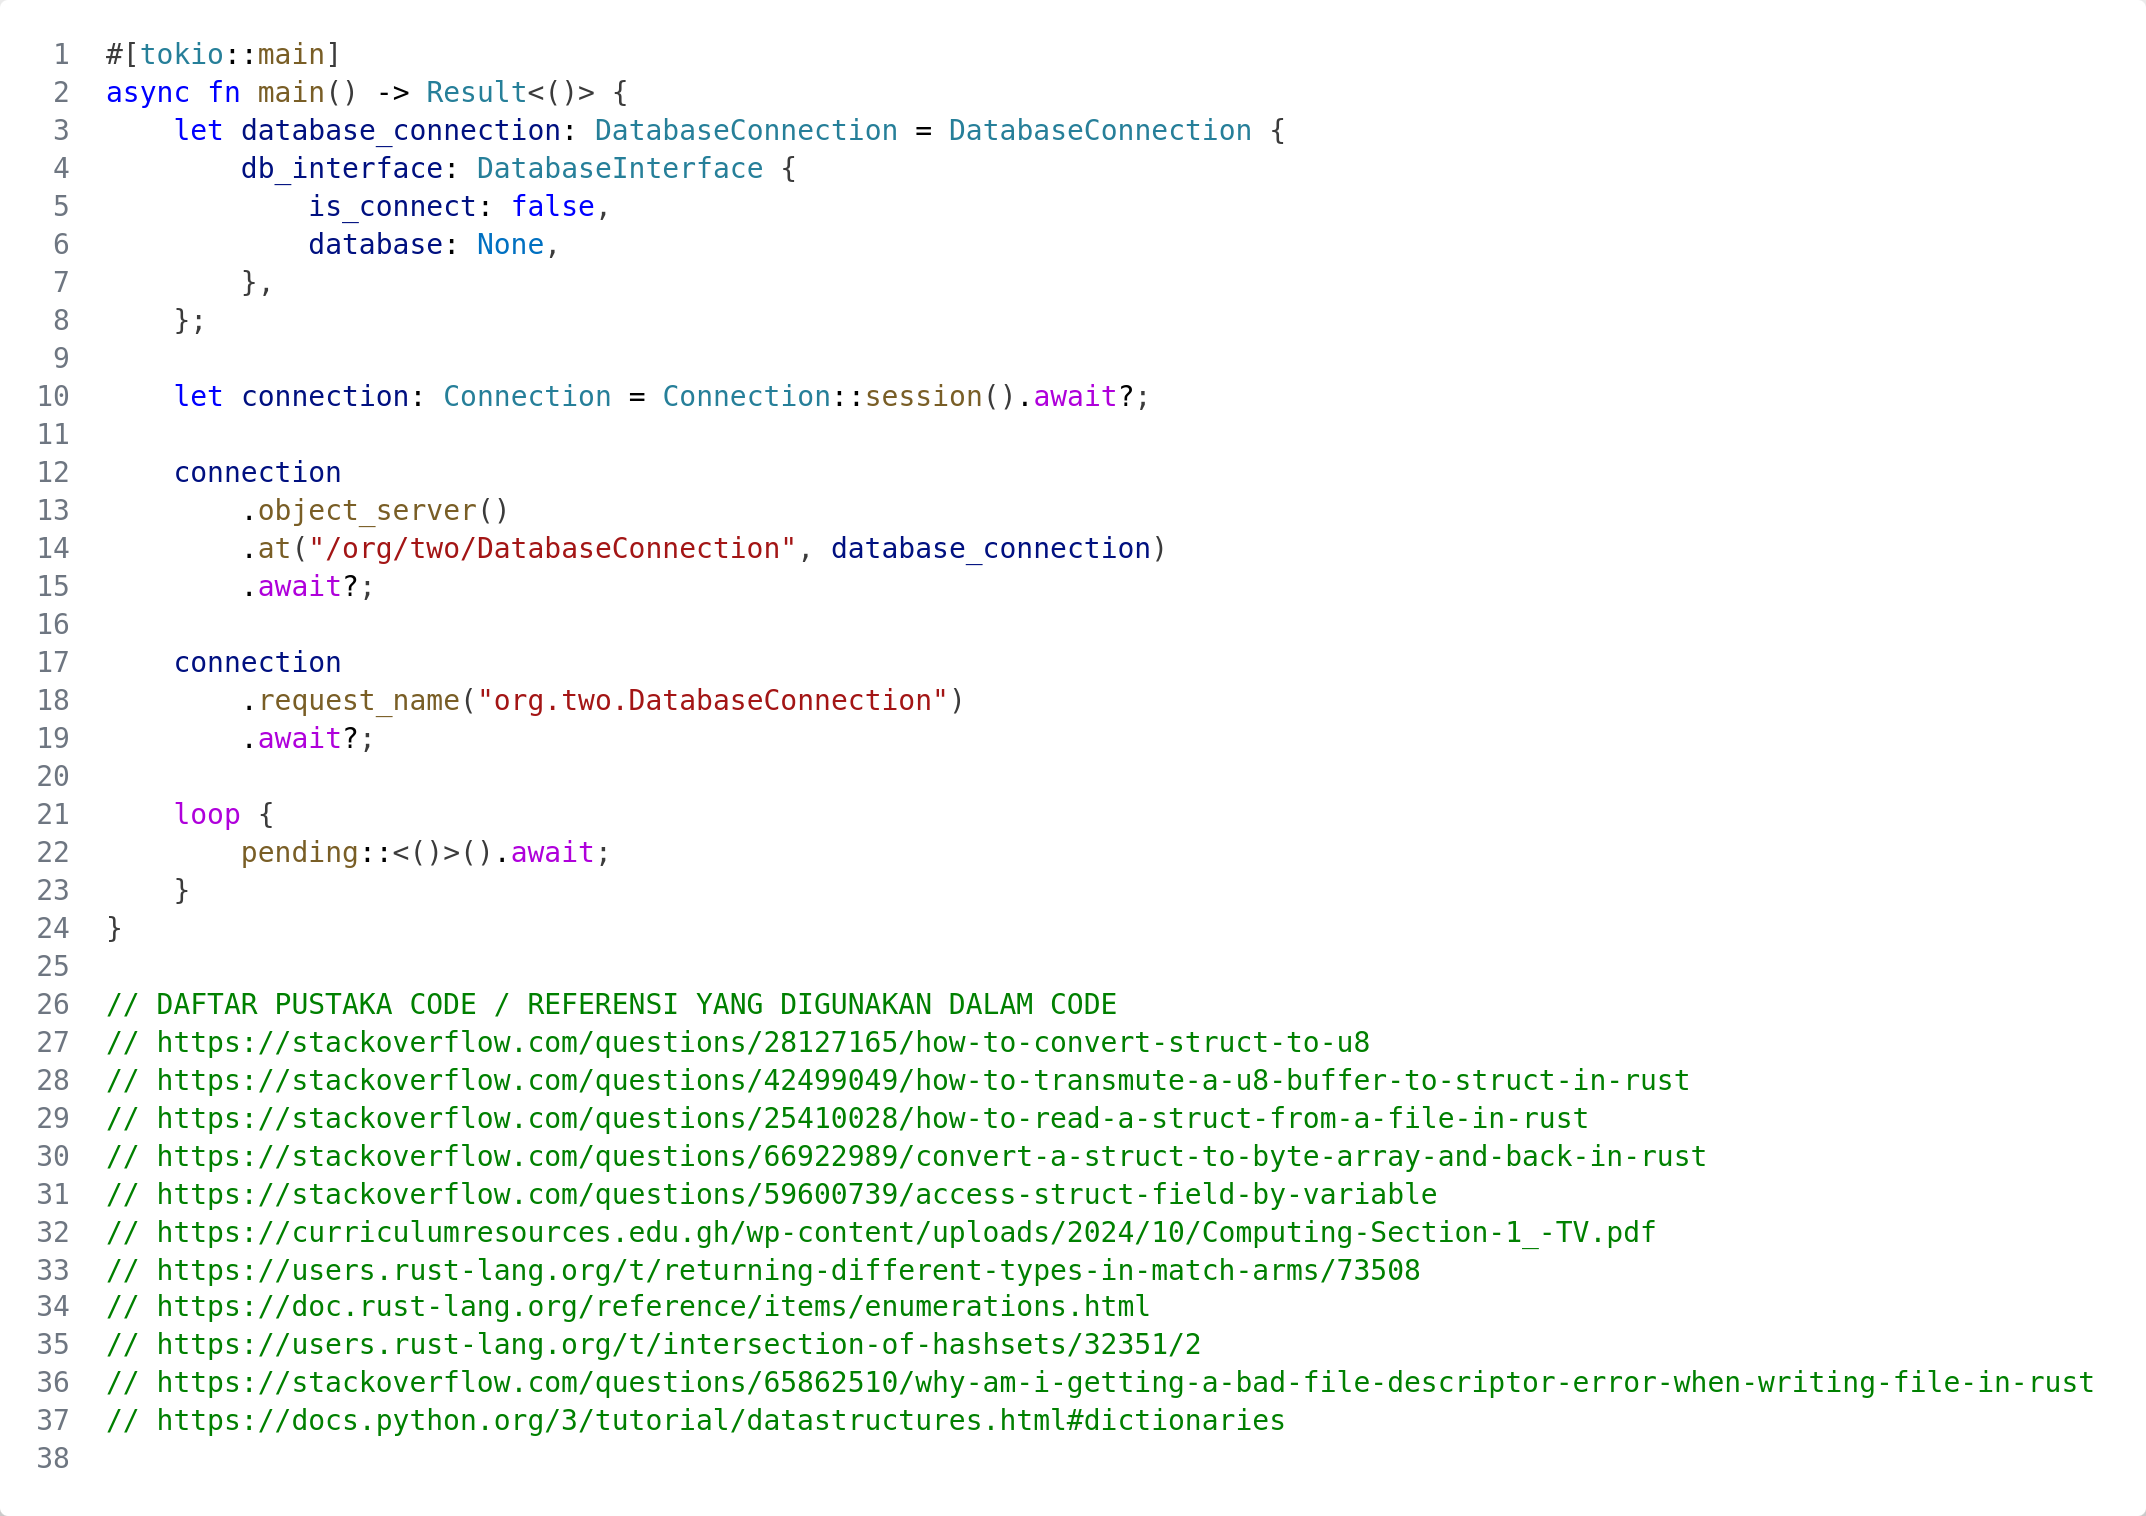
\includegraphics[width=0.9\textwidth]{gambar/lampiran/file-main-function.png}
  \caption{\emph{Function} main dalam \emph{file} main.rs}
\end{figure}

\begin{figure}[H]
  \centering{}
	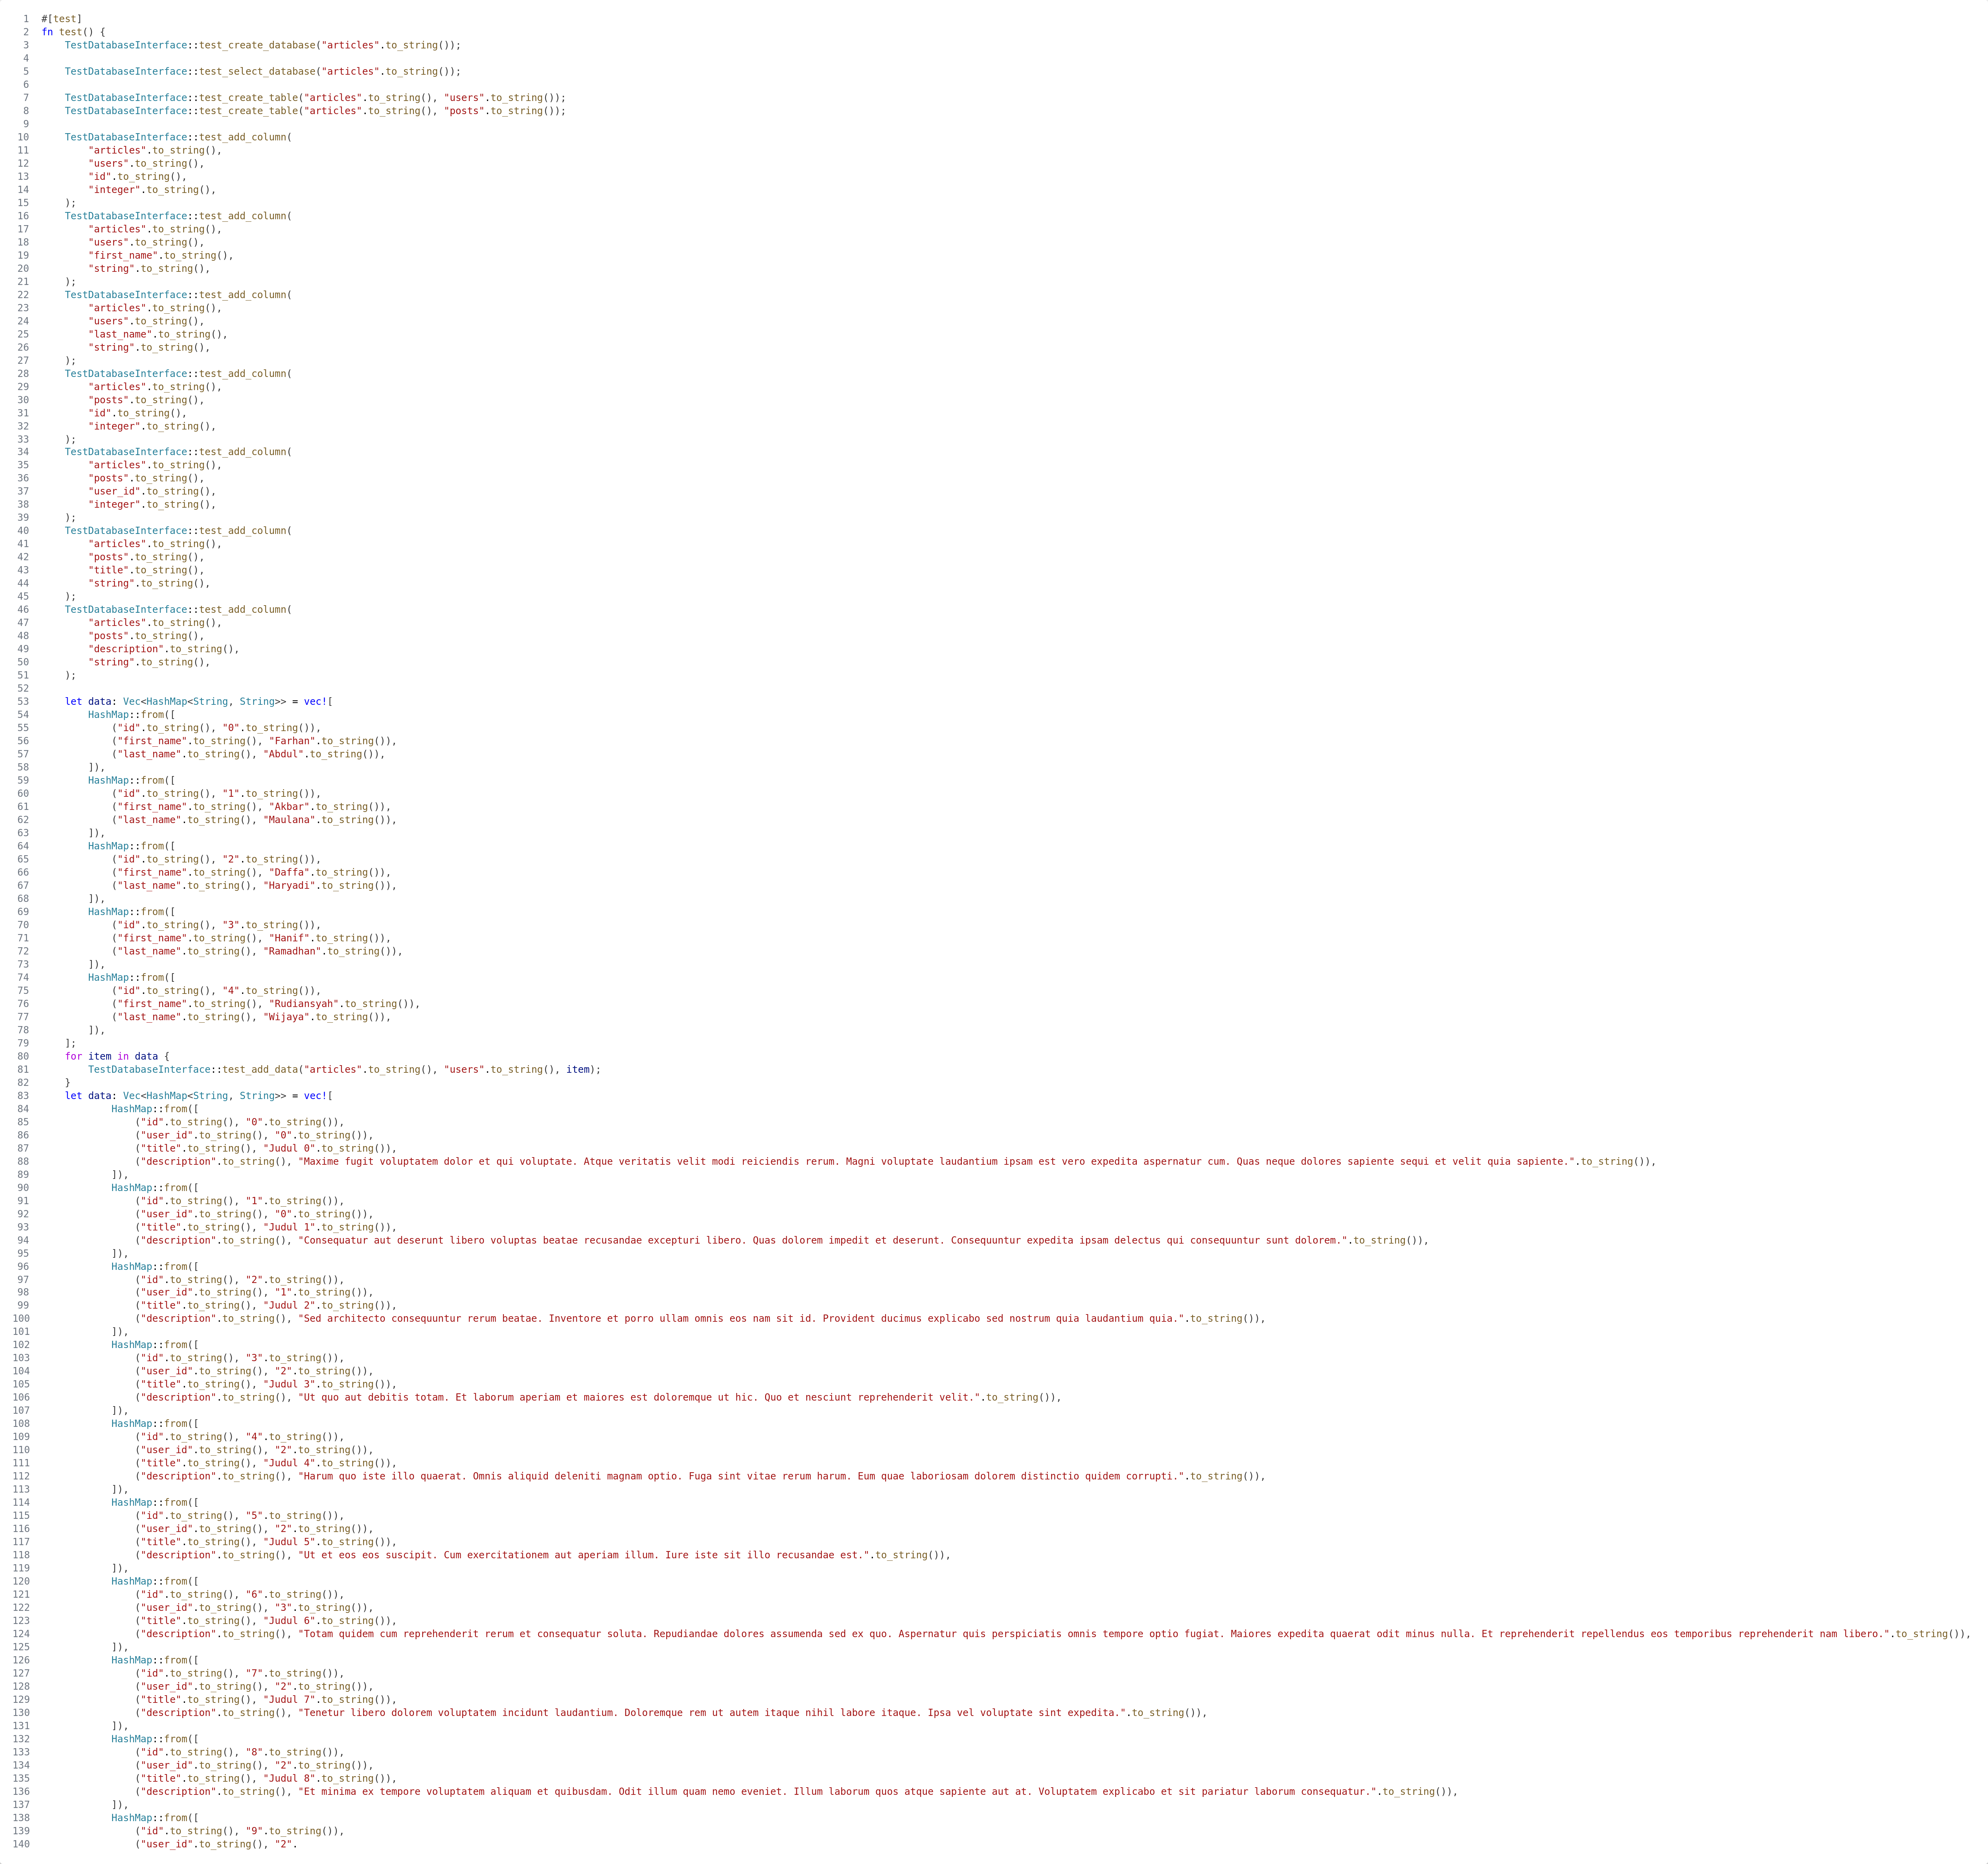
\includegraphics[width=0.9\textwidth]{gambar/lampiran/file-main-test-1.png}
  \caption{\emph{Function} test dalam \emph{file} main.rs bagian 1}
\end{figure}

\begin{figure}[H]
  \centering{}
	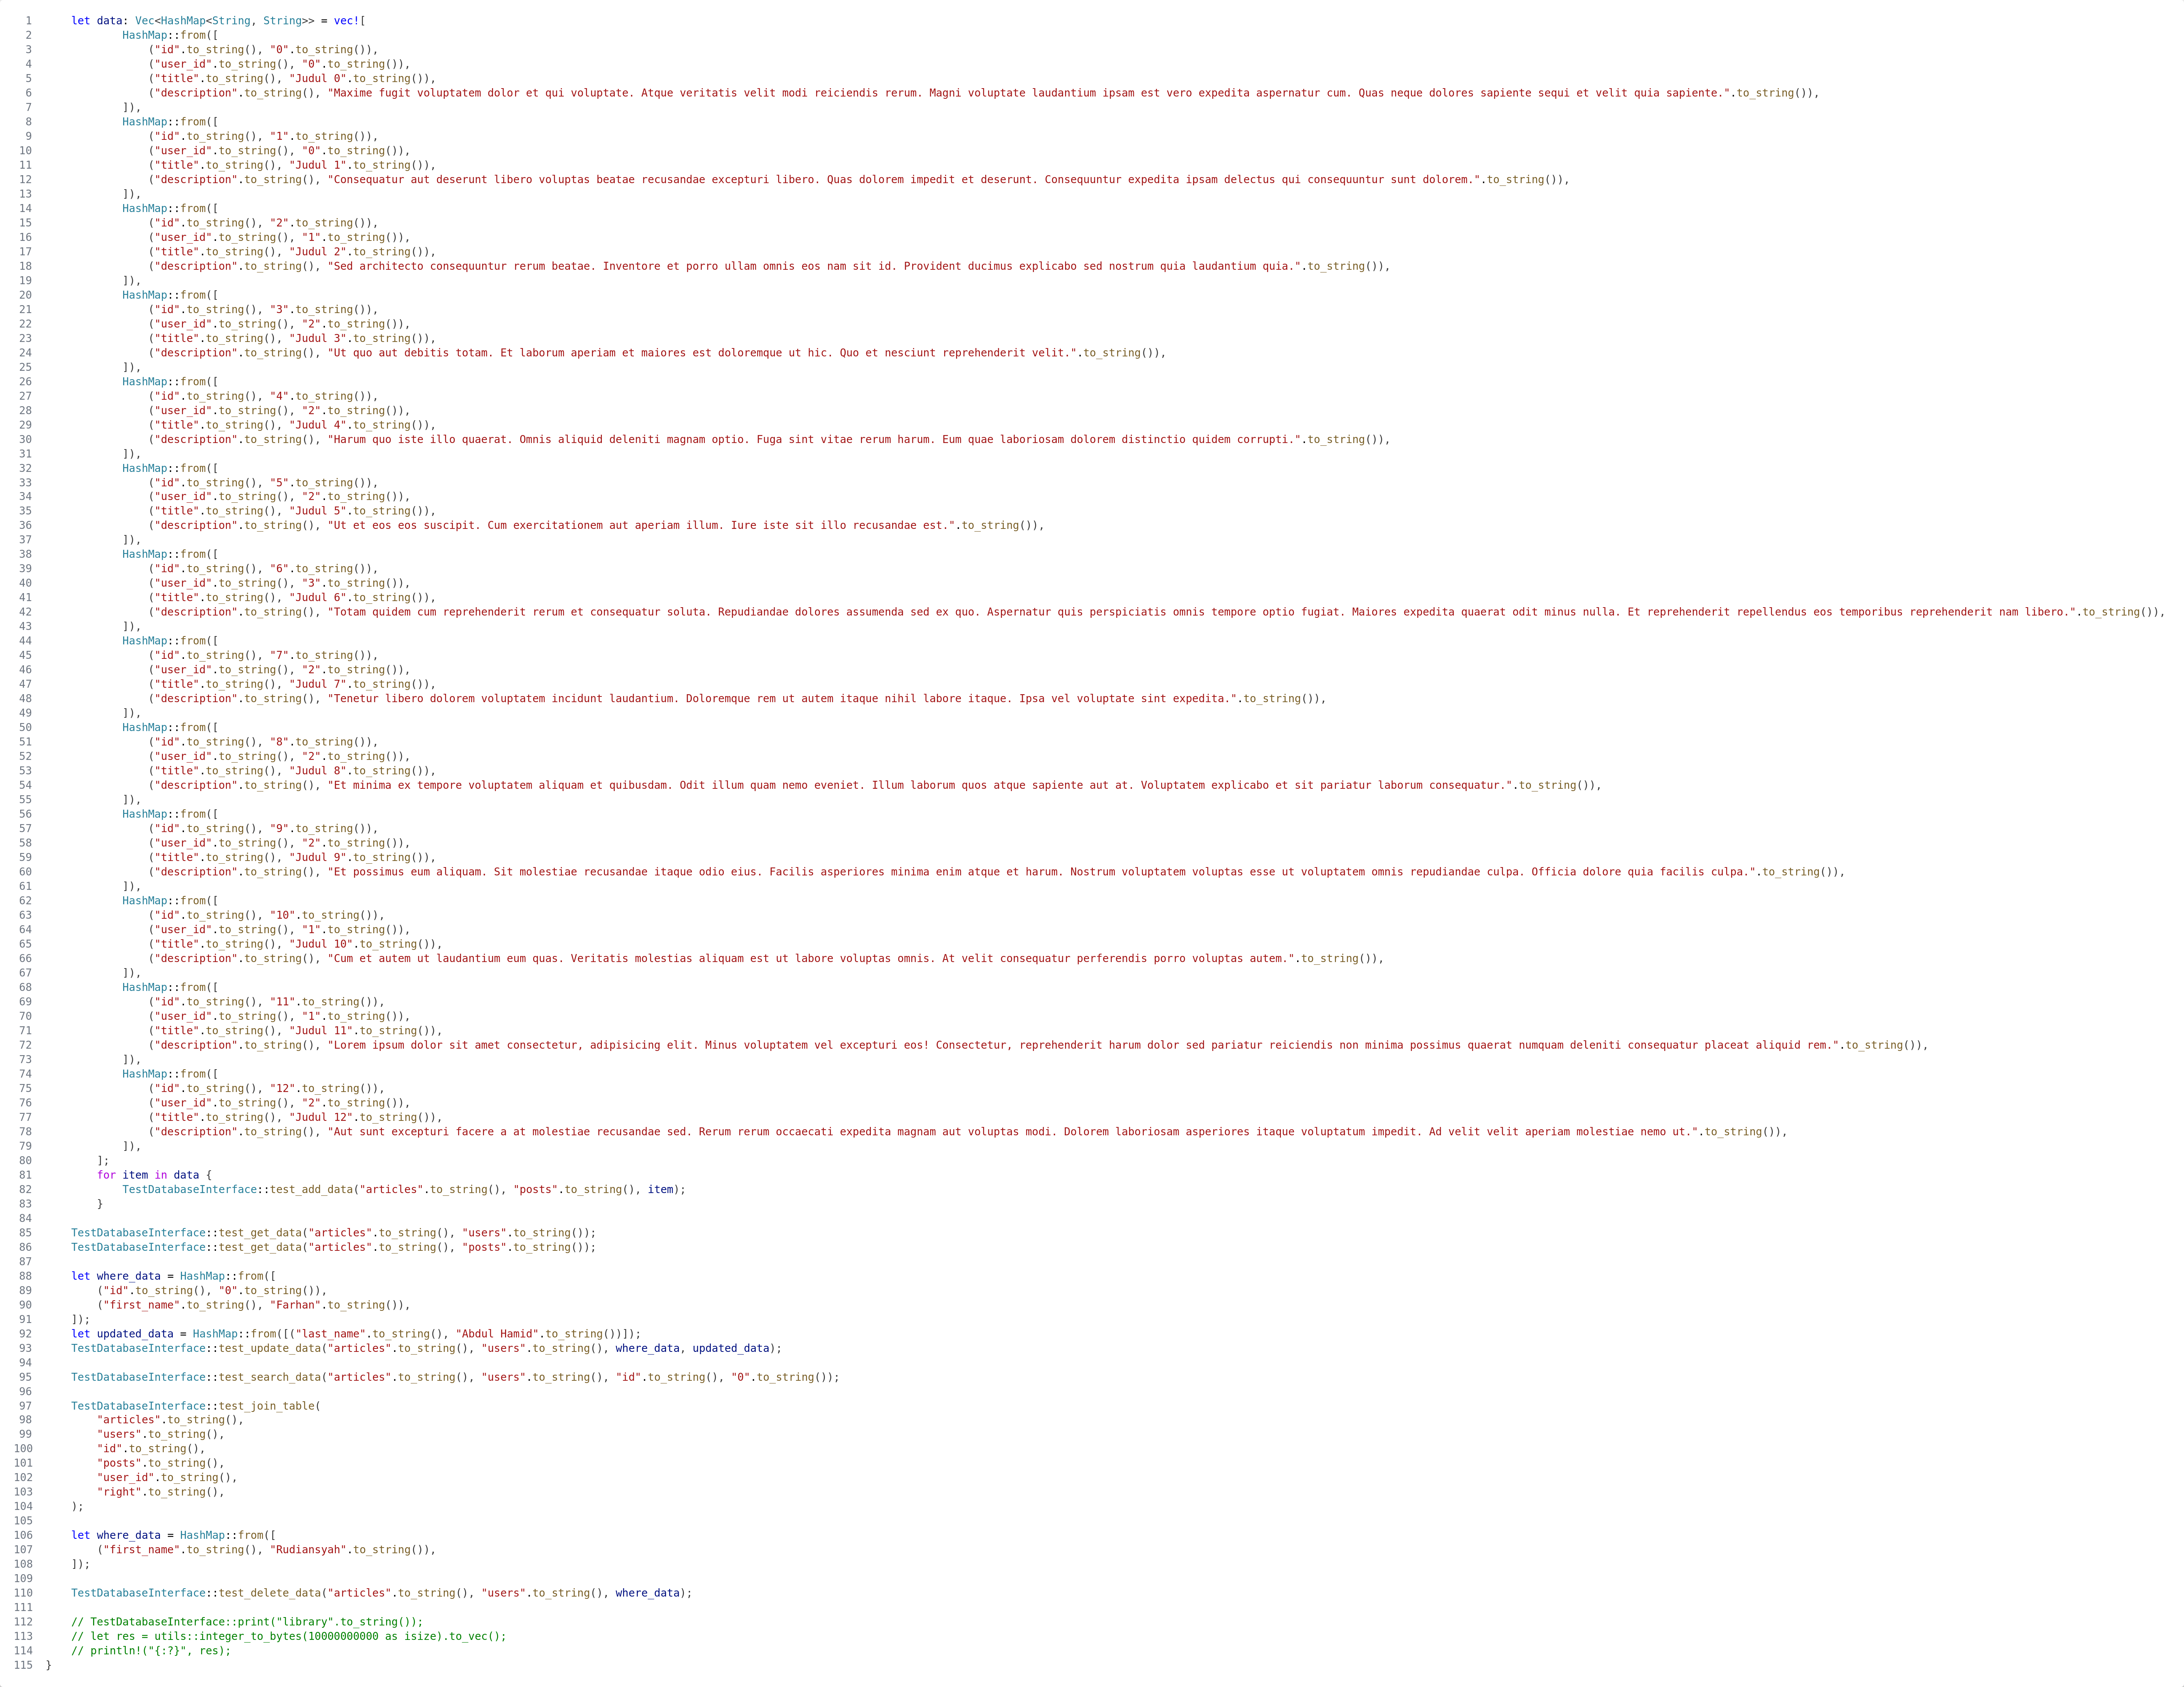
\includegraphics[width=0.9\textwidth]{gambar/lampiran/file-main-test-2.png}
  \caption{\emph{Function} test dalam \emph{file} main.rs bagian 2}
\end{figure}

\begin{figure}[H]
  \centering{}
	\includegraphics[width=0.4\textwidth]{gambar/lampiran/file-main-test-data-1.png}
  \caption{\emph{Function} test\_data\_crawling dalam \emph{file} main.rs. Keseluruhan \emph{function} dapat dilihat di \emph{source code} langsung}
\end{figure}


\begin{figure}[H]
  \centering{}
	\includegraphics[width=0.9\textwidth]{gambar/lampiran/file-cell.png}
  \caption{\emph{File} cell.rs}
\end{figure}

\begin{figure}[H]
  \centering{}
	\includegraphics[width=0.6\textwidth]{gambar/lampiran/file-column-1.png}
  \caption{\emph{File} column.rs bagian 1}
\end{figure}

\begin{figure}[H]
  \centering{}
	\includegraphics[width=0.4\textwidth]{gambar/lampiran/file-column-2.png}
  \caption{\emph{File} column.rs bagian 2}
\end{figure}

\begin{figure}[H]
  \centering{}
	\includegraphics[width=0.7\textwidth]{gambar/lampiran/file-table-1.png}
  \caption{\emph{File} table.rs bagian 1}
\end{figure}

\begin{figure}[H]
  \centering{}
	\includegraphics[width=0.6\textwidth]{gambar/lampiran/file-table-2.png}
  \caption{\emph{File} table.rs bagian 2}
\end{figure}

\begin{figure}[H]
  \centering{}
	\includegraphics[width=0.7\textwidth]{gambar/lampiran/file-table-3.png}
  \caption{\emph{File} table.rs bagian 3}
\end{figure}

\begin{figure}[H]
  \centering{}
	\includegraphics[width=0.7\textwidth]{gambar/lampiran/file-table-4.png}
  \caption{\emph{File} table.rs bagian 4}
\end{figure}

\begin{figure}[H]
  \centering{}
	\includegraphics[width=0.7\textwidth]{gambar/lampiran/file-table-5.png}
  \caption{\emph{File} table.rs bagian 5}
\end{figure}

\begin{figure}[H]
  \centering{}
	\includegraphics[width=0.6\textwidth]{gambar/lampiran/file-schema-1.png}
  \caption{\emph{File} schema.rs bagian 1}
\end{figure}

\begin{figure}[H]
  \centering{}
	\includegraphics[width=0.6\textwidth]{gambar/lampiran/file-schema-2.png}
  \caption{\emph{File} schema.rs bagian 2}
\end{figure}

\begin{figure}[H]
  \centering{}
	\includegraphics[width=0.6\textwidth]{gambar/lampiran/file-schema-3.png}
  \caption{\emph{File} schema.rs bagian 3}
\end{figure}

\begin{figure}[H]
  \centering{}
	\includegraphics[width=0.4\textwidth]{gambar/lampiran/file-schema-4.png}
  \caption{\emph{File} schema.rs bagian 4}
\end{figure}

\begin{figure}[H]
  \centering{}
	\includegraphics[width=0.6\textwidth]{gambar/lampiran/file-schema-5.png}
  \caption{\emph{File} schema.rs bagian 5}
\end{figure}

\begin{figure}[H]
  \centering{}
	\includegraphics[width=0.6\textwidth]{gambar/lampiran/file-database-connection-1.png}
  \caption{\emph{File} database\_connection.rs bagian 1}
\end{figure}

\begin{figure}[H]
  \centering{}
	\includegraphics[width=0.7\textwidth]{gambar/lampiran/file-database-connection-2.png}
  \caption{\emph{File} database\_connection.rs bagian 2}
\end{figure}

\begin{figure}[H]
  \centering{}
	\includegraphics[width=0.6\textwidth]{gambar/lampiran/file-database-interface-1.png}
  \caption{\emph{File} database\_interface.rs bagian 1}
\end{figure}

\begin{figure}[H]
  \centering{}
	\includegraphics[width=0.4\textwidth]{gambar/lampiran/file-database-interface-2.png}
  \caption{\emph{File} database\_interface.rs bagian 2}
\end{figure}

\begin{figure}[H]
  \centering{}
	\includegraphics[width=0.6\textwidth]{gambar/lampiran/file-database-interface-3.png}
  \caption{\emph{File} database\_interface.rs bagian 3}
\end{figure}

\begin{figure}[H]
  \centering{}
	\includegraphics[width=0.6\textwidth]{gambar/lampiran/file-database-interface-4.png}
  \caption{\emph{File} database\_interface.rs bagian 4}
\end{figure}


\begin{figure}[H]
  \centering{}
	\includegraphics[width=0.9\textwidth]{gambar/lampiran/file-mod.png}
  \caption{\emph{File} mod}
\end{figure}


\begin{figure}[H]
  \centering{}
	\includegraphics[width=0.3\textwidth]{gambar/lampiran/file-test-database-interface-1.png}
  \caption{\emph{File} test\_interface.rs bagian 1}
\end{figure}

\begin{figure}[H]
  \centering{}
	\includegraphics[width=0.4\textwidth]{gambar/lampiran/file-test-database-interface-2.png}
  \caption{\emph{File} test\_interface.rs bagian 2}
\end{figure}

\begin{figure}[H]
  \centering{}
	\includegraphics[width=0.6\textwidth]{gambar/lampiran/file-test-database-interface-3.png}
  \caption{\emph{File} test\_interface.rs bagian 3}
\end{figure}

\begin{figure}[H]
  \centering{}
	\includegraphics[width=0.6\textwidth]{gambar/lampiran/file-test-database-interface-4.png}
  \caption{\emph{File} test\_interface.rs bagian 4}
\end{figure}

\begin{figure}[H]
  \centering{}
	\includegraphics[width=0.6\textwidth]{gambar/lampiran/file-test-database-interface-5.png}
  \caption{\emph{File} test\_interface.rs bagian 5}
\end{figure}

\begin{figure}[H]
  \centering{}
	\includegraphics[width=0.6\textwidth]{gambar/lampiran/file-test-database-interface-6.png}
  \caption{\emph{File} test\_interface.rs bagian 6}
\end{figure}

\begin{figure}[H]
  \centering{}
	\includegraphics[width=0.6\textwidth]{gambar/lampiran/file-test-database-interface-7.png}
  \caption{\emph{File} test\_interface.rs bagian 7}
\end{figure}

\begin{figure}[H]
  \centering{}
	\includegraphics[width=0.4\textwidth]{gambar/lampiran/file-utils.png}
  \caption{\emph{File} utils.rs}
\end{figure}


\pagestyle{empty}
\chapter*{\centering \large DAFTAR RIWAYAT HIDUP}
\thispagestyle{empty}
\onehalfspacing{}

\begin{wrapfigure}{l}{4cm}
	\vspace{-25pt}
	\begin{center}
		\includegraphics[width=0.27\textwidth]{gambar/pasfoto.JPG}
	\end{center}
	\vspace{-40pt}
\end{wrapfigure}

\noindent \textbf{FARHAN DEWANTA SYAHPUTRA.} Lahir di Jakarta, 11 Oktober 2001.
Anak Ketiga dari pasangan Bapak Yusirwansyah dan Ibu Dewi Banyuwati.
Saat ini penulis tinggal di Jl. Teratai Putih 1 Nomor 161 RT 004/RW 004, Kelurahan Malaka Sari,
Kecamatan Duren Sawit, Kota Jakarta Timur, Provinsi DKI Jakarta.

\vspace{1cm}
\noindent
\begin{tabular}{lcl}
	No. Ponsel	& :&  081291335215 \\
	Email	& :&  farhan.abdulhamid11@gmail.com
\end{tabular}
\vspace{0.5cm}

\noindent \textbf{Riwayat Pendidikan} : Penulis mengikuti pendidikan sekolah
dasar di SDS Tadika Puri pada tahun 2007 - 2013. Setelah itu,
penulis melanjutkan pendidikan di SMPN 213 Jakarta pada tahun
2013 - 2016. Kemudian penulis melanjutkan pendidikan di SMAN 12 Jakarta pada
tahun 2016 - 2019. Setelah lulus, penulis melanjutkan perkuliahan 
di Universitas Negeri Jakarta pada tahun 2019.

\noindent \textbf{Riwayat Organisasi} : Selama di bangku perkuliahan, penulis 
terlibat dalam organisasi Default Program Studi Ilmu Komputer 
sebagai Staff dan Ketua Departemen Mobile Development periode 2021-2022. 


\pagestyle{empty}
\chapter*{\centering \large METADATA}
\thispagestyle{empty}
\onehalfspacing{}

\vspace{2cm}
\noindent
\begin{tabular}{lcl}
	Judul	& :&  Perancangan dan Implementasi Prototype \\
	& & \emph{Database Engine} Berbasis \emph{Structure Oriented} \\
	& & \emph{Programming} Menggunakan Rust \\
	Nama	& :&  Farhan Dewanta Syahputra \\
	NIM	& :&  1313619017 \\
	Pembimbing I	& :&  Muhammad Eka Suryana, M.Kom \\
	Pembimbing II	& :&  Med Irzal, M.Kom \\
	Keyword	& :& 1. Database \\
	& & 2. Index \\
	& & 3. Basis Data \\
	& & 4. Sistem Terdistribusi
\end{tabular}
\vspace{0.5cm}



\end{document}
